\begin{quote}
	\textit{``Amplified, shielded, channeled, prosthetized, simulated, stimulated, irritated - our sensorium is more mediated today than ever before. Yet it bothers us less. The cyborg model of the 1980s and the virtual dreams of the 1990s have evolved into a twenty-first-century `comfort zone', in which the prosthetic and supplemental are habitual.''}
\end{quote}
\hfill \textit{The Mediated Sensorium, Caroline A. Jones}
\\
\\

%=========================================================================================================

\label{chapter-eval-1}

This chapter recounts the first of two stages of evaluation conducted with the Mirrorshades platform, tasked with establishing the worth of the parallel reality concept in comparison to previously explored alternate reality techniques, as well as ascertaining the feasibility of the concept in general. To this end the platform was deployed to a user study in which a reconstruction of a 15th century chapel and its present day counterpart were explored by participants both via a seated VR experience, as VR content has already come to be employed at cultural heritage sites, and via a parallel reality experience using Mirrorshades.

%=========================================================================================================

%Final video
%\url{https://www.youtube.com/watch?v=UsDRPjDwr8A}
%screenshots

%=========================================================================================================

\section{Overview}



Participants were sourced by adverts disseminated via an internal university memo system which sends email to all registered staff and students each week. The advert appeared for several consecutive weeks. Participants were invited to take part in a \textit{``virtual reality study \ldots\ investigating different ways of switching your view between your real surroundings and a virtual environment''}. Participation was incentivised by a prize draw to win Amazon vouchers. This approach was adopted instead of sourcing participants from within the OVW group and wider (computer science) department as participants with a heightened knowledge and/or interest in the technology underlying the platform were expected to skew results by paying conscious attention to the system and its implementation, rather than the actual experience of using it. User studies each lasted 20-30 minutes and took place at St Salvator's chapel during afternoon hours while the chapel was open to the general public. Ethical approval for all stages of the evaluation is included as appendix \ref{appendix-ethics}.

%In total 17 participants, 10x male and 7x female, with a mean age of 23.1 years and a standard deviation of 4.9 years,

\begin{figure}
	\begin{center}
		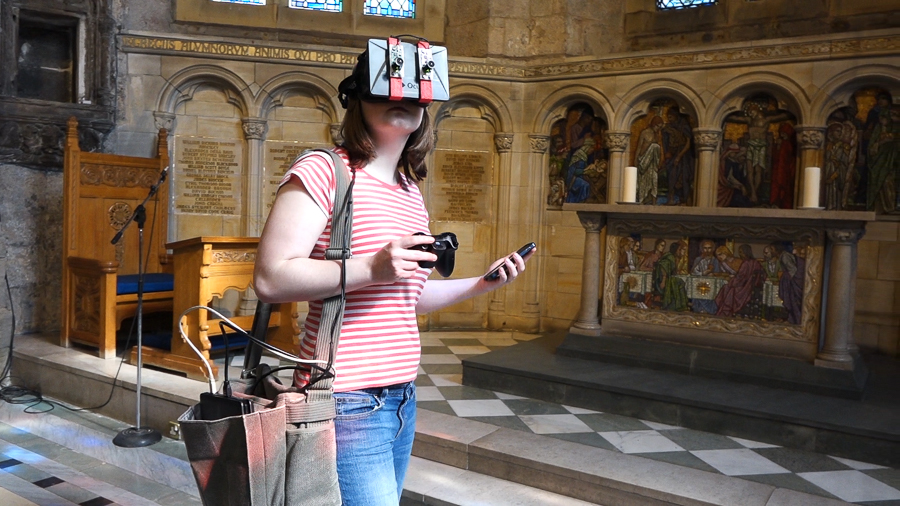
\includegraphics[width=\linewidth]{participant-f.jpg}
		\caption{Participant using Mirrorshades in a user study at St Salvator's chapel.}
		\label{participant-f.jpg}
	\end{center}
\end{figure}

%=========================================================================================================

\section{Stage 1 - Merit of Parallel Reality}

Previously when immersive VR has been employed in virtual heritage scenarios it has predominantly been implemented as CAVE experiences~\cite{Roussou2002}. Visitors to a museum or visitor centre are presented the opportunity to step into a CAVE, possibly donning shutter glasses or similar apparatus to enable a stereoscopic 3D effect, to experience a VR reconstruction of a location, its contents and actors. Some of these CAVE installations have featured physical control interfaces such as joystick and 3D mouse~\cite{cabral:x3dexperience} and haptic interfaces~\cite{Christou2006}, while others have tracked user movement, whether head only or full body  gestures (such as the OVW group's VTTP platform shown in figure \ref{VTTP_projection.png}). In common among these CAVE experiences is that the VR content they present is experienced with a disconnect to the RW site to which it pertains, as the CAVE itself completely immerses users in VR visuals and does not permit them to see any of their RW surroundings, comparable to the experience of wearing a VR HMD without video see-through functionality. Furthermore the physical size of a CAVE limits the amount in any particular direction that a user can physically move, `prisoned' in Tzortzaki's language~\cite{Tzortzaki2002}, even if movement is encouraged due to its use as a control methodology. This presents a hindrance to the on-site comparison of real and virtual content, as it introduces both temporal and spatial separation between a user's experiences of the VR content and the corresponding RW objects and environment.

With the promise of high performance VR HMDs at a consumer price point on the horizon, thanks largely to the rejuvenation in the field effected by Oculus, their use at cultural heritage sites for achieving similar experiences to previous CAVE installations is becoming more plausible and brings with it certain benefits such as a reduction in the physical space required at the site for the installation. The OVW group's experience with presenting both experts and the general public with virtual heritage content via Oculus HMDs (see section \ref{virtual-heritage-at-st-andrews}) has been very promising. These interactions have taken place in scenarios similar to those of existing cultural heritage CAVE scenarios; the user remains physically stationary and uses a controller or gestures to move their virtual presence throughout the VR environment, whilst unable to observe the RW environment due to the nature of the HMD isolating them from RW visual stimuli.

In this first stage of the evaluation a comparison was made between this stationary style of interaction with VR content at a cultural heritage site wherein VR is experienced in isolation from RW, with both temporal and spatial separation, and a parallel reality style of interaction afforded by the Mirrorshades parallel reality platform, in which VR is experienced in tandem with RW by allowing the user to move around the RW environment and freely transition at any time into seeing the VR environment from the equivalent vantage point. Participants in this stage of the evaluation thus completed two scenarios wherein they interacted with the RW St Salvator's chapel and its corresponding VR reconstruction:

\begin{enumerate}
	\item \textbf{Seated VR scenario} - Participants experienced the RW and VR chapels separately. They navigated the VR chapel from a seated position, as VR has already come to be employed at cultural heritage sites via CAVE installations and by the OVW group with Oculus HMDs, using the Xbox controller to move around the VR environment observed via the DK1 which obscured their view of the RW chapel around them. Subsequently they navigated the RW chapel without the DK1 or any associated equipment, in order to pay comparison between it and the VR environment they had just experienced.
	\item \textbf{Parallel reality scenario} - Participants experienced the RW and VR chapels in tandem using the Mirrorshades platform. They wore the DK1, held the Xbox controller in their right hand and the smartphone in their left, with the laptop and control box bundle in a satchel worn over one shoulder (see figure \ref{participant-f.jpg}). Pressing and holding a button on the Xbox controller triggered a transition from RW visual stimuli to VR visual displayed by the DK1.
\end{enumerate}

Thus in addition to simply assessing the feasibility of the concept, this first stage of evaluation was designed to ascertain whether applying parallel reality to a cultural heritage scenario resulted in an improvement in participant engagement and understanding of the relationships between the RW and VR environments compared to a traditional seated VR cultural heritage scenario. Improvements were expected to arise from addressing the problems of spatial and temporal separation inherent with a seated VR scenario by imparting upon the participant the ability to freely transition with no delay between equivalent vantage points within the RW and VR environments.

%=========================================================================================================

\subsection{Design of the Scenarios}

The scenarios were intended to mimic the style of exploration and interaction that visitors to the chapel usually display, based upon observation of the behaviour of visitors on several occasions. From these observations a common pattern of behaviour emerged; visitors would enter the chapel from the North/West corner then proceed to walk Eastwards along the nave, pausing to look around after passing through the rood screen, before continuing along the nave toward the altar. They would pause in front of the altar upon reaching the end of the pews and then walk North toward the tomb where they would pause again to inspect it. Participants in this first stage of the evaluation process were instructed to imagine that they were performing a similar visit to the chapel and to follow a similar path, pausing after the rood screen, at the end of the pews and in front of the tomb to look around their environment(s) in more detail. They were however encouraged to stop and look around at any times/positions that they wished and not to feel restricted to the described path and locations - the intent of the scenario was to encourage a natural style of exploration despite the unusual situation of making use of bulky VR hardware, rather than to restrict them to an `on rails' experience. Participants were shown the map included as figure \ref{chapel-path} to help visualise the scenario.

\begin{figure}
	\begin{center}
		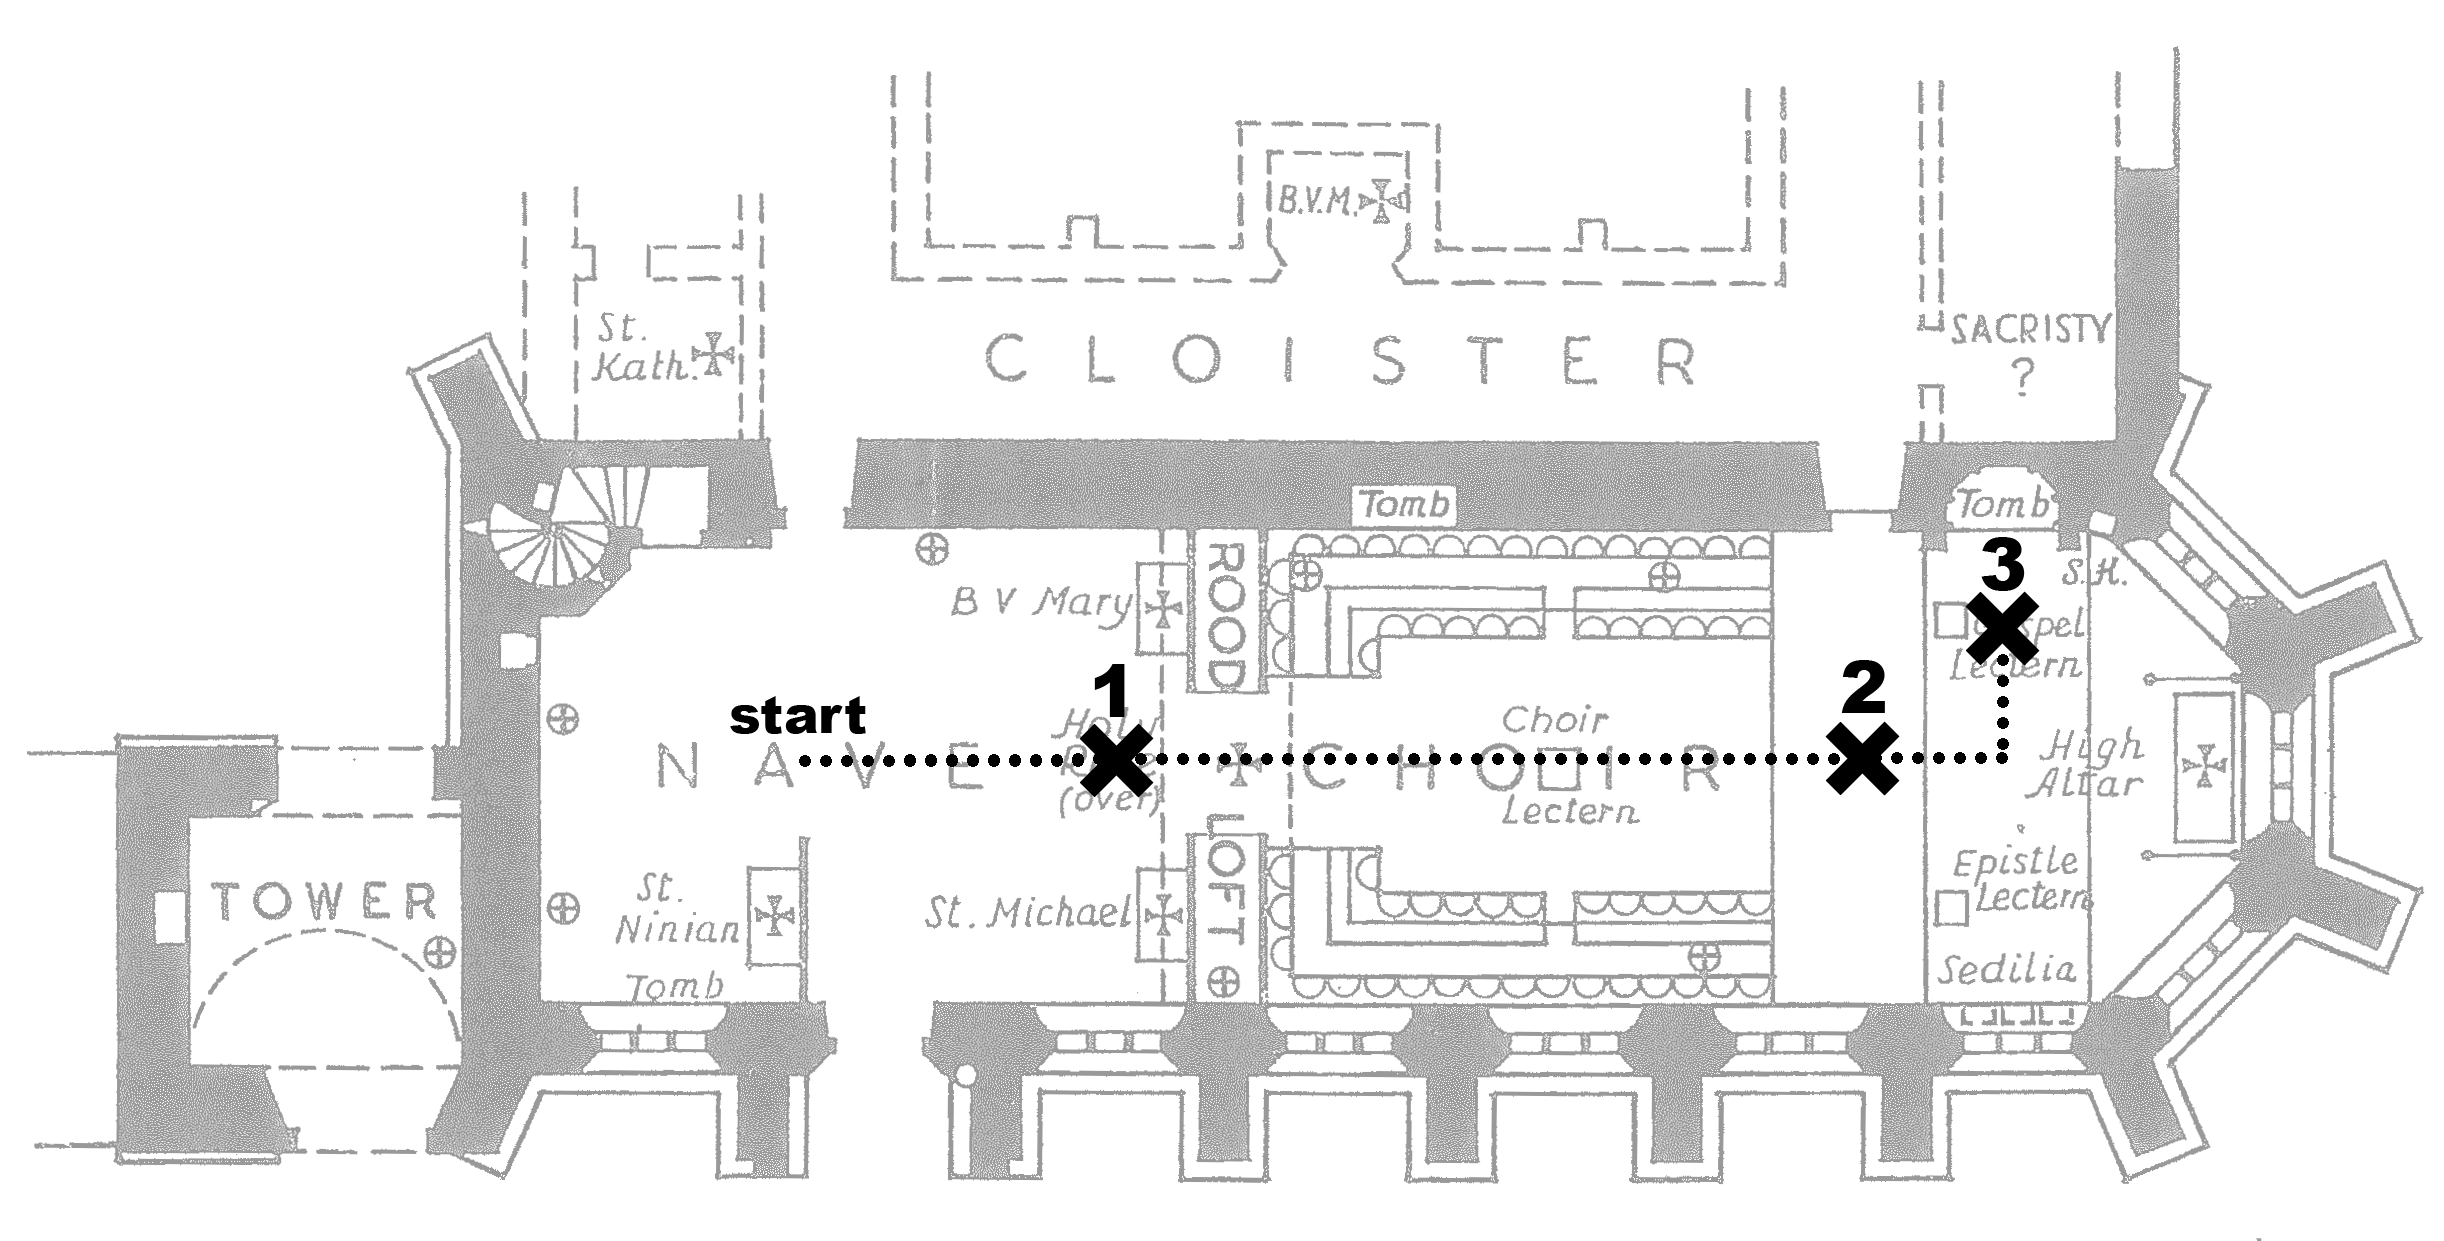
\includegraphics[width=.6\linewidth]{chapel-path.png}
		\caption{Path (dotted line) and positions (numbered crosses) within St Salvator's chapel that participants were instructed to roughly follow and attend to (oriented North upwards).}
		\label{chapel-path}
	\end{center}
\end{figure}

In the seated VR scenario participants interacted with the VR chapel using the DK1 and Xbox controller. After completing the path in the VR chapel they removed the DK1 and walked through the real chapel. This behaviour alludes to how VR has already come to be applied to cultural heritage sites such as St Salvator's chapel, wherein visitors have the opportunity to experience a CAVE or stationary HMD based reconstruction of the site either before or after having explored the RW site. In the parallel reality scenario they walked roughly the same path, but this time with the ability to freely transition between viewing the RW chapel and the VR chapel from the equivalent vantage points.

In the parallel reality scenario participants had access to a single transition style, the transition with linear interpolation (section \ref{transition-with-linear-interpolation}), triggered by pressing and holding the \texttt{A} button on the Xbox controller. As mentioned in section \ref{initial-testing} this transition emerged as the `favourite' during initial tests within the OVW group and as such it was chosen as the only transition style for the parallel reality scenario in this first stage of evaluation. The focus of this stage of the evaluation was upon comparing the parallel reality scenario to a seated VR experience and not upon gleaning details of the merits and drawbacks exhibited by different transitions. The default view on the DK1's screen was 100\% RW with the transition causing a change to 100\% VR, a situation whose expected experience is visualised upon the combined Milgram/Waterworth model in figure \ref{focus-locus-sensus-with-virtuality-continuum-with-transition}.

Before taking part in the two scenarios, participants were given the opportunity to familiarise themselves with the DK1 by spending a few minutes interacting with Oculus' `Tuscany' demo\footnote{\url{https://share.oculus.com/app/oculus-tuscany-demo}}. This demo was developed by Oculus themselves and was distributed with the Rift Unity integration package. It represented at the time a very polished and stable DK1 experience, ideal for introducing inexperienced users to HMD based VR. It was used to give participants an opportunity to acclimatize to the Rift (some people react badly to a first VR HMD experience, with feelings of nausea) in order to reduce skewing their subsequent experiences with the St Salvator's chapel model due to drastically different levels of familiarity with the DK1 between the two scenarios.

%=========================================================================================================

\subsection{Evaluation Techniques}
\label{stage-1-evaluation-techniques}
All participants completed a pre-task questionnaire which provided calibration for other data by enquiring about age, gender identity, previous experience with VR HMDs and whether they had previously visited St Salvtor's chapel, both RW and VR (the RW chapel is open to the public and a version of the VR reconstruction is publicly accessible via the OVW group's OpenSim grid\footnote{\url{http://openvirtualworlds.org}}). The System Usability Scale (SUS)~\cite{Brooke1996} was used to provide a basic comparison between the usability of the two scenarios, while a 12-item Likert-type questionnaire (included as appendix \ref{appendix-12-item-likert-type-questionnaire-stage-1}) was used to collect opinions on more specific aspects of the experience of both scenarios. At the end of the session, after completing both scenarios, participants were engaged in a short structured interview (prompts included as appendix \ref{appendix-interview-questions-stage-1}) in order to allow them to elaborate upon their experience in a more free form manner. The visuals displayed upon the DK1 were recorded via ShadowPlay and the participants themselves were recorded by video camera. Finally, log data were collected during both scenarios, capturing the information detailed in table \ref{logdatatable} to file at regular intervals for statistical processing and visualising via R.

\newpage

\begin{center}
\begin{longtable}{ l  p{6.5cm} }

\toprule

\textbf{Field} & \textbf{Description} \\

\midrule

\texttt{<frame number>} & Incremented with each frame pushed to the DK1, starting at 0 when the Unity application is started. \\

\midrule

\texttt{<timestamp>} & According to the laptop's internal clock. \\

\midrule

\texttt{<original\_position>} & The position as a Unity \texttt{Vector3} where the participant begins the experiment (as reported by IndoorAtlas). \\

\midrule

\texttt{<position>} & The position as a Unity \texttt{Vector3} where the participant is on this frame (as reported by IndoorAtlas). \\

\midrule

\texttt{<delta\_x>} and \texttt{<delta\_z>} & The difference in the \texttt{x} and \texttt{z} axes between \texttt{<original\_position>} and \texttt{<position>} on this frame. Change in elevation (\texttt{y} axis) is not recorded, as IndoorAtlas does not provide elevation data and the area of St Salvator's chapel used throughout the studies is level. \\

\midrule

\texttt{<left\_rotation>} and \texttt{<right\_rotation>} & The orientation as Unity \texttt{Quaternion} of the two Unity camera game objects. The orientation of these Unity objects is directly tied to the orientation of the DK1, so these values represent the orientation of the participant's head on each frame. \\

\midrule

\texttt{<base\_opacity>} & The maximum opacity of the game objects upon which the camera feeds are rendered. Reduced maximum opacity (see section \ref{subsub-baseopacity}) is implemented by setting this field to a value \textless 1. \\

\midrule

\texttt{<left\_opacity>} and \texttt{<right\_opacity>} & The opacity on this frame of the game objects upon which the camera feeds are rendered. \\

\midrule

\texttt{<auto\_tick>} & Whether a periodic transition is in progress (see section \ref{subsub-periodic}). \\

\midrule

\texttt{<auto\_duration>} and \texttt{<auto\_spacing>} & The interval and duration values of the periodic transitions (if applicable). \\

\midrule

\texttt{<framerate>} & An estimate of the current frame rate (frames per second). \\

\midrule

\texttt{<A\_button>}, \texttt{<B\_button>} and \texttt{<right\_trigger>} & The current values of these inputs on the Xbox controller. For the \texttt{A} and \texttt{B} buttons this is binary, either pressed or not, while for the trigger it is a numeric value representing the amount that the trigger is being depressed. \\

\bottomrule
\caption{Log data captured during Mirrorshades evaluations.}
\label{logdatatable}
\end{longtable}
\end{center}

%=========================================================================================================

\section{Stage 1 Results}

A total of 6 participants completed the stage 1 evaluation:
\begin{itemize}
	\item Age ranged from 21 to 26, with a mean of 23.3 and a standard deviation of 1.86.
	\item 3 identified as male and 3 as female.
	\item All reported previous experience with a games console controller.
	\item 1 reported previous experience with a HMD.
	\item 2 reported having previously visited the real world chapel.
	\item None had previously experienced the virtual chapel.
\end{itemize}

Due to the small sample size and its skewed age group the observations drawn from these results should be primarily considered in terms of initial evidence that justifies and informs more comprehensive future work. Combined with the fact that this stage of the evaluation was weighted more toward assessing the feasibility of the parallel reality concept and its worth compared to previous alternate reality applications within cultural heritage, than toward making detailed recommendations about specifics of implementations, these observations contribute to the set of abstract, high level best practices for future parallel reality endeavours enumerated in section \ref{best-practices-for-parallel-reality}, rather than leading to strict and infallible claims as to the nature of the parallel reality concept and its implementation. However in reference to the age group it is interesting to consider the observation, noted in section \ref{virtual-heritage}, that younger visitors to cultural heritage sites often experience less arousal at sites where the former splendour is no longer visible, which may mean that they have more to gain from an application of parallel reality to cultural heritage than other age groups.

Original data are not reproduced within this thesis due to size constraints and the ethical agreement under which the evaluations were performed, however these data (including interview transcripts) can be made available by contacting the author\footnote{\texttt{cj@cjdavies.org}}.

%=========================================================================================================

\subsection{SUS}
The parallel reality scenario scored slightly lower on SUS than the seated VR scenario (see figure \ref{sus.png}). The cumbersome nature of the hardware was expected to have this impact upon SUS scores, with the parallel reality scenario averaging lower than the seated VR scenario. Participants who were able to overcome this cumbersomeness were expected to respond more favourably to the parallel reality scenario than those who could not and the small size of the discrepancy between the two results indicates that most participants did not find the cumbersome nature of the parallel reality scenario to be a substantial detractor to their experience.

\TwoFig{1/sus.png}{Stage 1 evaluation SUS results.}{sus.png}
       {1/post_task_questionnaire_boxplot.png}{Stage 1 evaluation Likert-type questionnaire results.}{post_task_questionnaire_boxplot.png}

%=========================================================================================================

\subsection{Likert-type Questionnaires}

One participant did not complete the Likert-type questionnaires. Coincidentally this participant was also the only one to have reported previous experience with a HMD in the pre-task questionnaire, so the Likert-type questionnaire responses wholly represent participants with no prior HMD experience. With the resurgence of interest in HMD based VR in recent years the number of developers and enthusiasts with HMD experience is climbing. However until the first commercial VR HMDs are released and begin to permeate gaming and media consumption audiences the situation captured by these questionnaire results, where all visitors to a cultural heritage site had no previous HMD experience, should be considered representative of the general public today.

The responses to the questionnaire are presented by figure \ref{post_task_questionnaire_boxplot.png} with the questions reproduced below. All questions were answered on a scale from 1 to 5, anchored between `strongly disagree' and `strongly agree' respectively:
\begin{enumerate}
	\item I found the exploration an enjoyable experience.
	\item It was easy to compare features from the past and the present.
	\item I felt motion sickness/dizziness.
	\item In the virtual environment, I had a sense of being there.
	\item I was aware of both real and virtual environments.
	\item It was rewarding to explore the chapel in this way.
	\item I felt as though I was in the past.
	\item I think I would have preferred a conventional computer monitor.
	\item This experience changed my understanding of the chapel.
	\item I did not notice differences between the real and virtual environments.
	\item The visual quality of the headset was bad.
	\item I feel I now better understand what the chapel was like in the past.
\end{enumerate}

Participants indicated that they generally found the parallel reality scenario to be more enjoyable (q1) and more rewarding (q6) than the seated VR scenario, with the former allowing them to more easily perform comparisons between features of the past and present (q2). Participants felt that they better understood what the chapel was like in the past after the parallel reality scenario than the seated VR scenario (q9/q12), however both scenarios scored equally low for participants thinking that they did not notice differences between RW and VR (q10). The parallel reality scenario led to a greater awareness of both environments (q5) and a greater sense of `being in the past' (q7) than the seated VR scenario.

The visual quality of the headset was perceived as being worse in the parallel reality scenario (q11). Whilst the visual quality of the VR visuals was identical in both scenarios, this result is presumably because during the parallel reality scenario the participants were viewing the RW environment upon the DK1's screen via the cameras, with much lower visual acuity than in the seated VR scenario where they observed the RW environment unmediated when subsequently walking through the chapel without the DK1 (see discussion in section \ref{constraints_of_dk1_see_through_solution}).

It is worth noting that although the parallel reality scenario scored lower than the seated VR scenario in SUS, both scenarios scored similarly high in question 2 (\textit{``It was easy to compare features from the past and the present''}) and similarly low in question 8 (\textit{``I think I would have preferred a conventional computer monitor''}) of the Likert-type questionnaire, indicating that the diminished usability of the parallel reality scenario did not pose a drastic hindrance to the experience overall.

%=========================================================================================================

\subsection{Interview Transcripts}
\label{stage1interviews}
Studying the structured interviews that were conducted after participants had completed both scenarios (interviews were recorded and subsequently transcribed) provided a wealth of qualitative feedback.

All participants said that the parallel reality scenario was more engaging than the seated VR scenario, even though 2 participants said that they preferred the seated VR scenario overall. Of these 2,  one did not find it comfortable to walk while wearing the DK1 and the other reported gaining a better understanding of the past from the seated VR scenario. The participant who found it uncomfortable to walk while wearing the DK1 was notably taller than all of the other participants in this stage. This is worth mentioning as the `height' of the virtual cameras in the VR reconstruction was fixed with reference to the UK average height of 5 feet 9 inches and was not changed to account for different participant heights as this would have required lengthy recalibration for each and every participant. For a participant of average height the discrepancy between their RW viewpoint and their VR viewpoint was minimal, however for a particularly short or particularly tall participant this discrepancy would have been much greater and may have contributed to the discomfort of walking with the DK1 as each transition between RW and VR would have resulted in a perceptible shift in height of the viewpoint.

Those that preferred the parallel reality scenario alluded to the immediacy of comparison between RW and VR as a contributing factor to this preference. Twice as many participants reported that the parallel reality scenario made it easier to spot differences between RW and VR than the seated VR scenario, with 4 out of 6 participants reporting that they noticed differences in the parallel reality scenario that they did not notice in the seated VR scenario. In particular, several participants mentioned the different position of the rood screen; one participant who didn't notice this difference during the seated VR scenario commented that the parallel reality scenario made it \textit{``blatantly obvious''}. Another participant was able to list multiple differences that s/he had spotted in the parallel reality scenario that they had not noticed in the seated VR scenario. One participant directly mentioned that the immediacy of comparison between RW and VR in the parallel reality scenario was what allowed them to spot more differences, another mentioned that with the seated VR scenario it was not clear that you were \textit{``trying to look into the past''} but in the parallel reality scenario it was obvious because \textit{``you can see the differences''}, while another said that s/he preferred the parallel reality scenario because \textit{``it was easier to compare and contrast between the real world and the virtual one''}.

The quality of the cameras was mentioned negatively by one participant who answered that the seated VR scenario made it easier to spot differences between RW and VR, with another participant specifically mentioning that a higher \textit{``resolution''} was needed.

The one participant to report experiencing motion sickness elaborated that it was worse when using the DK1 in the seated VR scenario than when walking with the DK1 in the parallel reality scenario, because \textit{``sitting down and moving around feels weird''}. This was a reference to moving throughout the VR environment using the Xbox controller whilst remaining physically stationary by sitting on the chair. John Carmack, the CTO of Oculus VR, went as far as to say that \textit{``Stick yaw control is such VR poison that removing it may be the right move -- swivel chair/stand or don't play.''}\footnote{\url{https://twitter.com/id_aa_carmack/status/553238861267353600}}. This observation demonstrates the negative effect that a conflict between proprioception (our ability to sense the relative positions of our body parts) and visual perception in a VR experience can have (see discussion in section \ref{presence-questionnaires}).

With regards to movement in the parallel reality scenario the accuracy, but more critically the lag, of the indoor positioning was cited by one participant as needing work, because it \textit{``caught me off guard twice''}. From watching the ShadowPlay recorded videos from the parallel reality scenario it is clear that in some cases the participants would trigger a transition to VR visual stimuli only to find that their VR position had not yet `caught up' with their RW position. This behaviour caused by the lag in IPS data was foreseen when considering the update frequency requirement of the IPS provision for the Mirrorshades platform (see section \ref{ips-requirements-for-mirrorshades}) however it was not expected to have as detrimental an effect as was expressed by some participants in the interviews.

%=========================================================================================================

\subsection{Log Data}

For the seated VR scenario log data were recorded while each participant was engaging with the VR chapel in the seated position and using the Xbox controller to navigate the VR environment. For the parallel reality scenario log data were recorded throughout the whole experiment, such that data are available both for the periods in which they were observing the RW chapel via the DK1 and cameras, and the periods in which they were observing the VR chapel after performing a transition.

%As such several comparisons can be made between these sets of data in addition to considering the data as a whole. Within the parallel reality scenario comparisons can be made between the periods that participants were observing RW and the periods that they were observing VR.

%Between the seated VR scenario and the parallel reality scenario comparisons can be made between the VR section of the seated VR scenario and the periods that participants were observing VR in the parallel reality scenario. Log data were not captured for participant 2, nor were they captured for the seated VR scenario for participant 5.

\subsubsection{Comparing seated and parallel reality scenarios}
\label{stage1-seated-vs-parallel-reality}
When looking at either scenario's data as a whole (the VR section of the seated VR scenario and both RW and VR periods of the parallel reality scenario) it is immediately evident that participants looked to their sides and turned their heads horizontally (yaw) far more than they looked above and beneath themselves by tilting their heads vertically (pitch). An example of this relationship is shown by figure \ref{6_pitch_yaw_2up.png} which shows pitch and yaw plotted against time for participant 6, for both the seated VR scenario and the parallel reality scenario. With the seated VR scenario on the left of the pair of plots and the parallel reality scenario on the right, the variance in yaw is substantially greater in both than the variance in pitch.

%\begin{figure}
%	\begin{center}
%	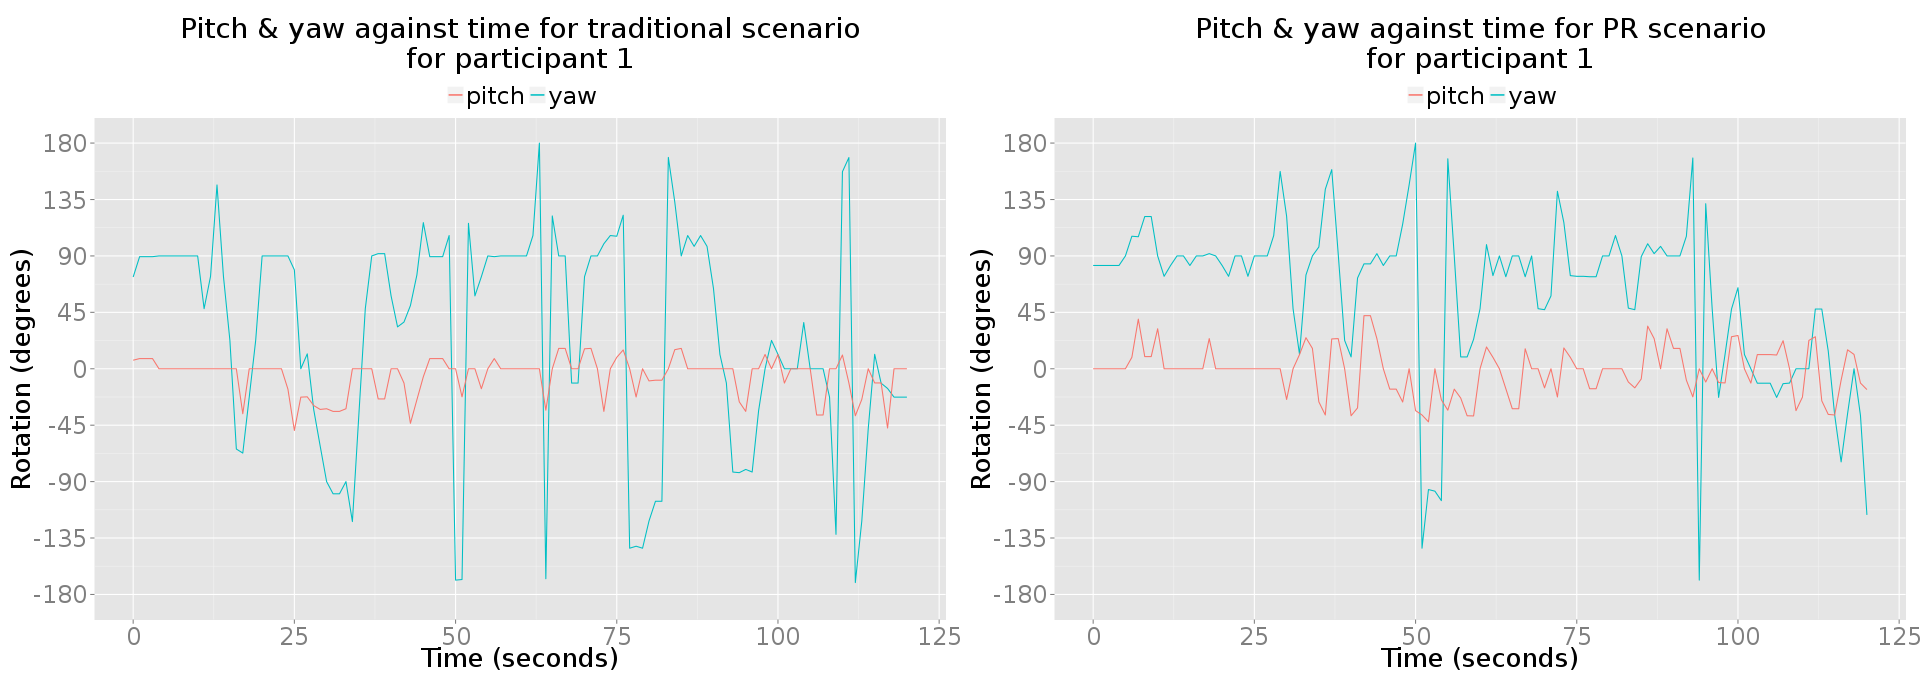
\includegraphics[width=\textwidth]{1/1_pitch_yaw_2up.png}
%	\caption{Pitch and yaw against time for participant 1 in seated VR and parallel reality scenarios.}
%	\label{1_pitch_yaw_2up.png}
%	\end{center}
%\end{figure}

%\begin{figure}
%	\begin{center}
%	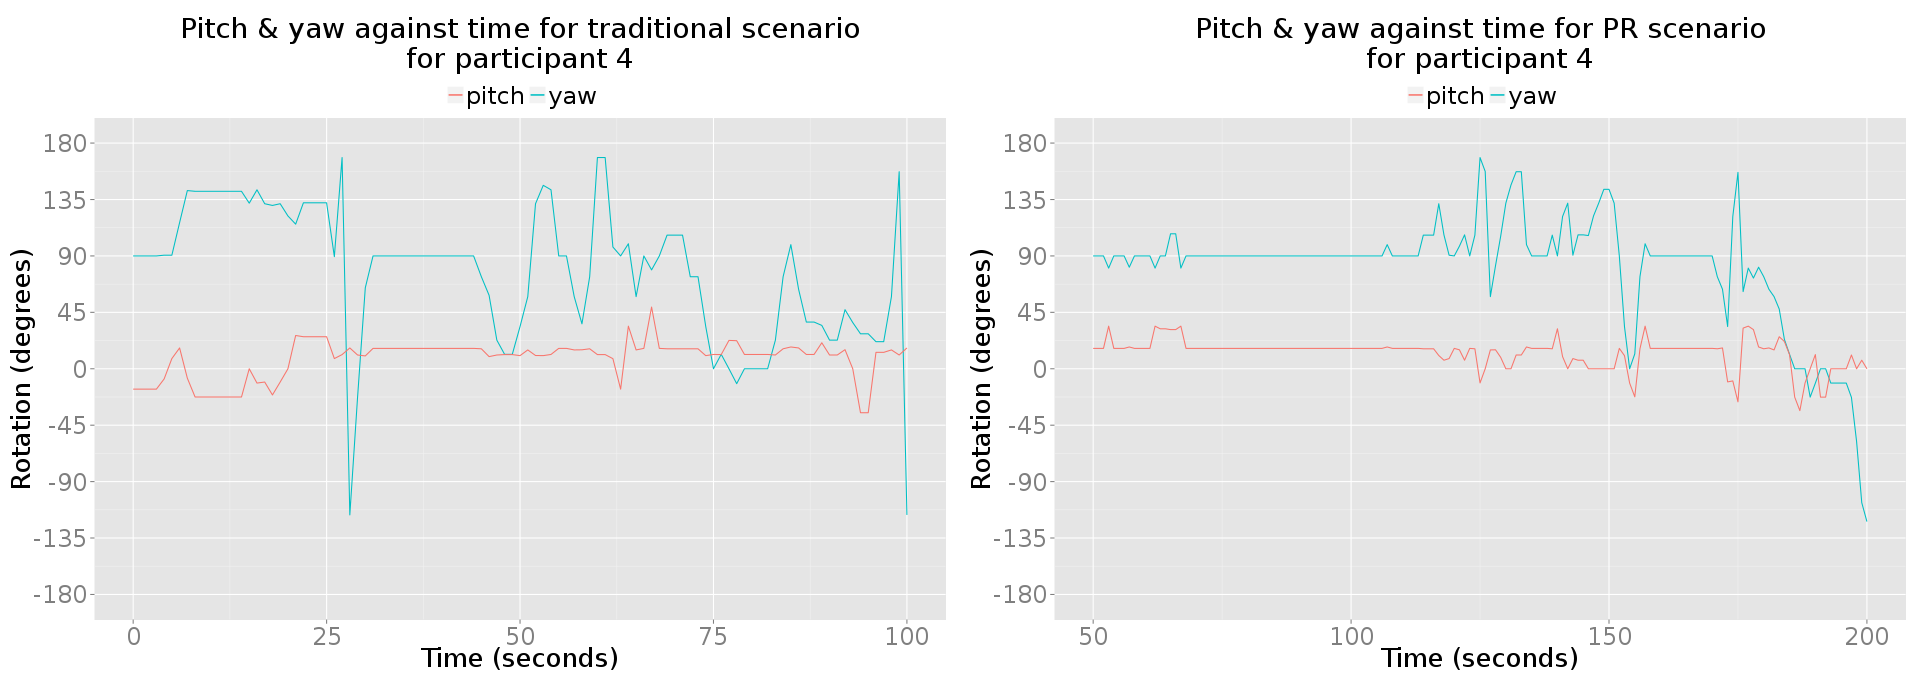
\includegraphics[width=\textwidth]{1/4_pitch_yaw_2up.png}
%	\caption{Pitch and yaw against time for participant 4 in seated VR and parallel reality scenarios.}
%	\label{4_pitch_yaw_2up.png}
%	\end{center}
%\end{figure}

\begin{figure}[h]
	\begin{center}
	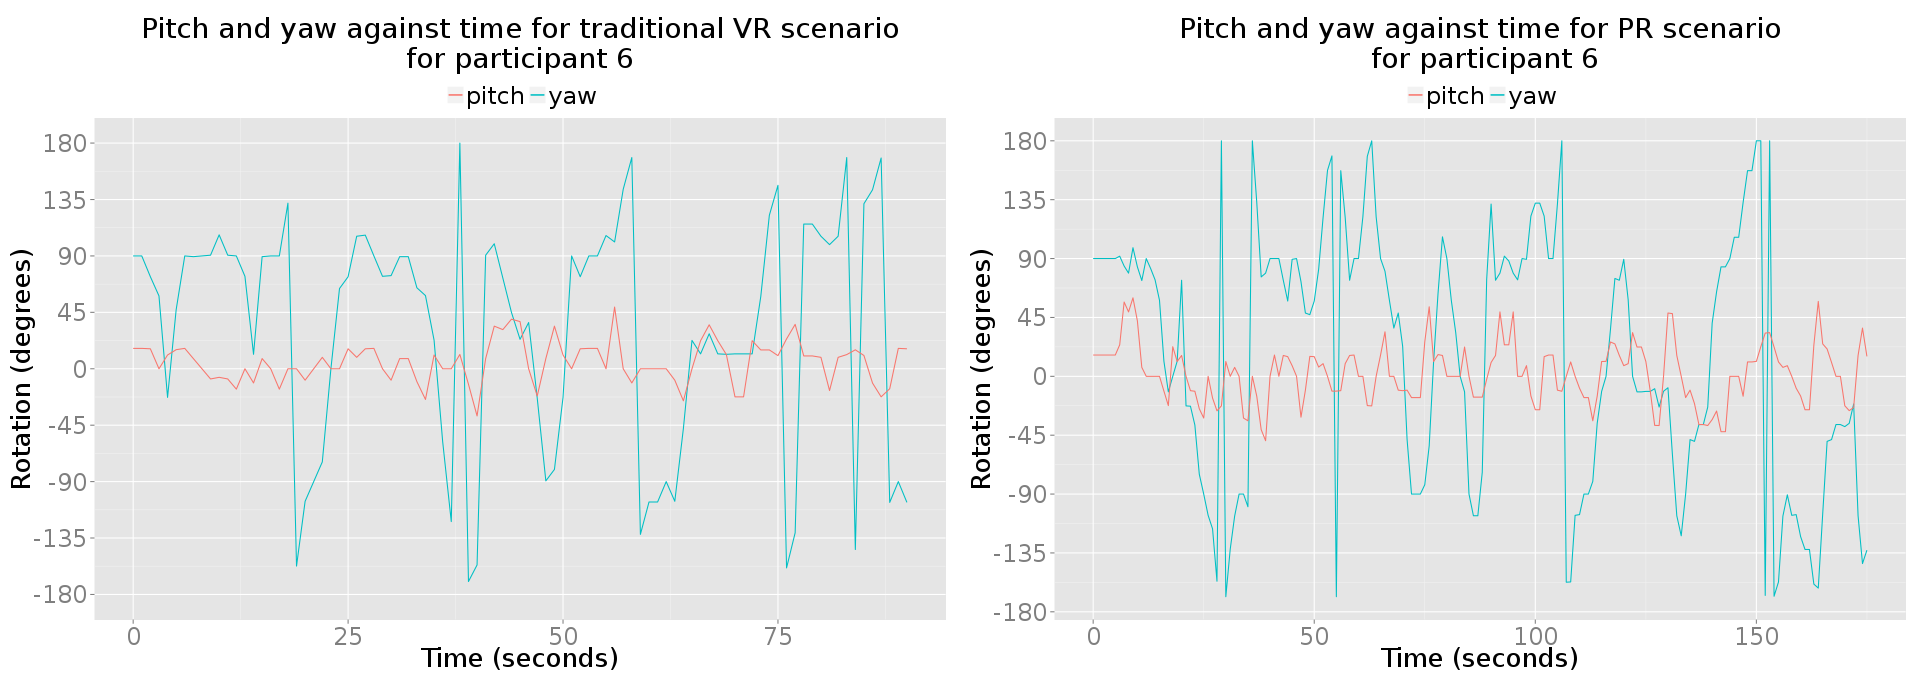
\includegraphics[width=\textwidth]{1/6_pitch_yaw_2up.png}
	\caption{Pitch and yaw against time for participant 6 in seated VR and parallel reality scenarios.}
	\label{6_pitch_yaw_2up.png}
	\end{center}
\end{figure}

This relationship is reflected in calculations of the standard deviation in pitch and yaw across both scenarios, shown by table \ref{sdpitchyawtrad} for the seated VR scenario and table \ref{sdpitchyawpr} for the parallel reality scenario. For all participants for which the data are available the standard deviation in yaw is substantially higher than that in pitch. This relationship can largely be explained by the simple fact that there is more to observe in the chapel(s) at ground level than above eye level or down at the ground, however with the marked difference in the appearance of the chapel roof (stone in the VR reconstruction and wood in the RW chapel today) a smaller difference between pitch and yaw variance might have been expected for both scenarios.

\begin{table}
\begin{center}
\begin{minipage}[t]{.45\linewidth}
\begin{center}
\begin{tabularx}{\textwidth}{c *{3}{>{\centering\arraybackslash}X}}
\toprule

\textbf{Participant} & \textbf{Pitch (\textdegree)} & \textbf{Yaw (\textdegree)} \\

\midrule

1 & 14.977 & 86.211 \\

3 & 16.684 & 60.545 \\

4 & 10.516 & 53.805 \\

5 & no data & no data \\

6 & 16.172 & 92.416 \\

\bottomrule
\end{tabularx}
\caption{Standard deviation in pitch and yaw for VR section of seated VR scenario.}
\label{sdpitchyawtrad}
\end{center}
\end{minipage}
%
\begin{minipage}[t]{.02\linewidth}
\hfill%
\end{minipage}
%
\begin{minipage}[t]{.45\linewidth}
\begin{center}
\begin{tabularx}{\textwidth}{c *{3}{>{\centering\arraybackslash}X}}
\toprule

\textbf{Participant} & \textbf{Pitch (\textdegree)} & \textbf{Yaw (\textdegree)} \\

\midrule

1 & 19.186 & 63.427 \\

3 & 24.228 & 51.666 \\

4 & 11.723 & 44.526 \\

5 & 16.542 & 39.601 \\

6 & 21.999 & 97.122 \\

\bottomrule
\end{tabularx}
\caption{Standard deviation in pitch and yaw for parallel reality scenario (RW and VR periods combined).}
\label{sdpitchyawpr}
\end{center}
\end{minipage}
\end{center}
\end{table}

%=====================

When studying plots of head pitch and yaw against time aligned with plots of distance moved against time, some participants seemed to display an aversion to large head movements while moving. Considering participant 1 as an example (figure \ref{1_4up.png}), they seem to have been quite comfortable looking around a lot even while moving in the seated VR scenario but in the parallel reality scenario their large head movements group around the periods in which their position was not changing as much\footnote{When looking at these plots it is important to appreciate that lag in the IndoorAtlas data results in a small lateral offset between the position data and the head orientation data, as the latter is unaffected by the lag in the correct reporting and `settling' of the former.}. When looking at the same data plotted for participant 3 however (figure \ref{3_4up.png}) it seems that they were reluctant to perform large head movements while moving in both scenarios, rather than just the parallel reality scenario.

Reluctance to changing head orientation when moving in the seated VR scenario can possibly be explained by something as simple as some participants (such as participant 1) having more experience with video games in which movement and looking direction are controlled independently. For somebody familiar with this style of control it is second nature to use one control to change their position whilst simultaneously using another control to change the direction in which they are looking, however for those unfamiliar or inexperienced with such scenarios it is common to observe alternation between movement and looking, something that the OVW group has observed in users interacting with virtual content at various demonstrations using keyboard and mouse, Xbox controller and other control methodologies. In many video games this simultaneous independent control of head and body is achieved by using keyboard buttons to control body movement while using a mouse to control looking direction, or by using the two separate control sticks of a controller such as an Xbox controller. With the seated VR scenario the Xbox controller provided control over movement and yaw, while the head tracker in the DK1 provided control over both pitch and yaw by tracking head orientation.

Reluctance to changing head orientation when moving in the parallel reality scenario is most logically explained by participants feeling as though with the reduced visual acuity of their RW environment seen through the cameras and DK1 screen combined with the discrepancy in position and environmental objects of their VR environment that they needed to pay more conscious attention to their walking, lest they lose their footing. Upon reaching a location of particular interest and standing still, their willingness to perform larger head movements returned as they no longer had to contend with obstacle avoidance.

\vspace{4cm}

\begin{figure}[h]
	\begin{center}
	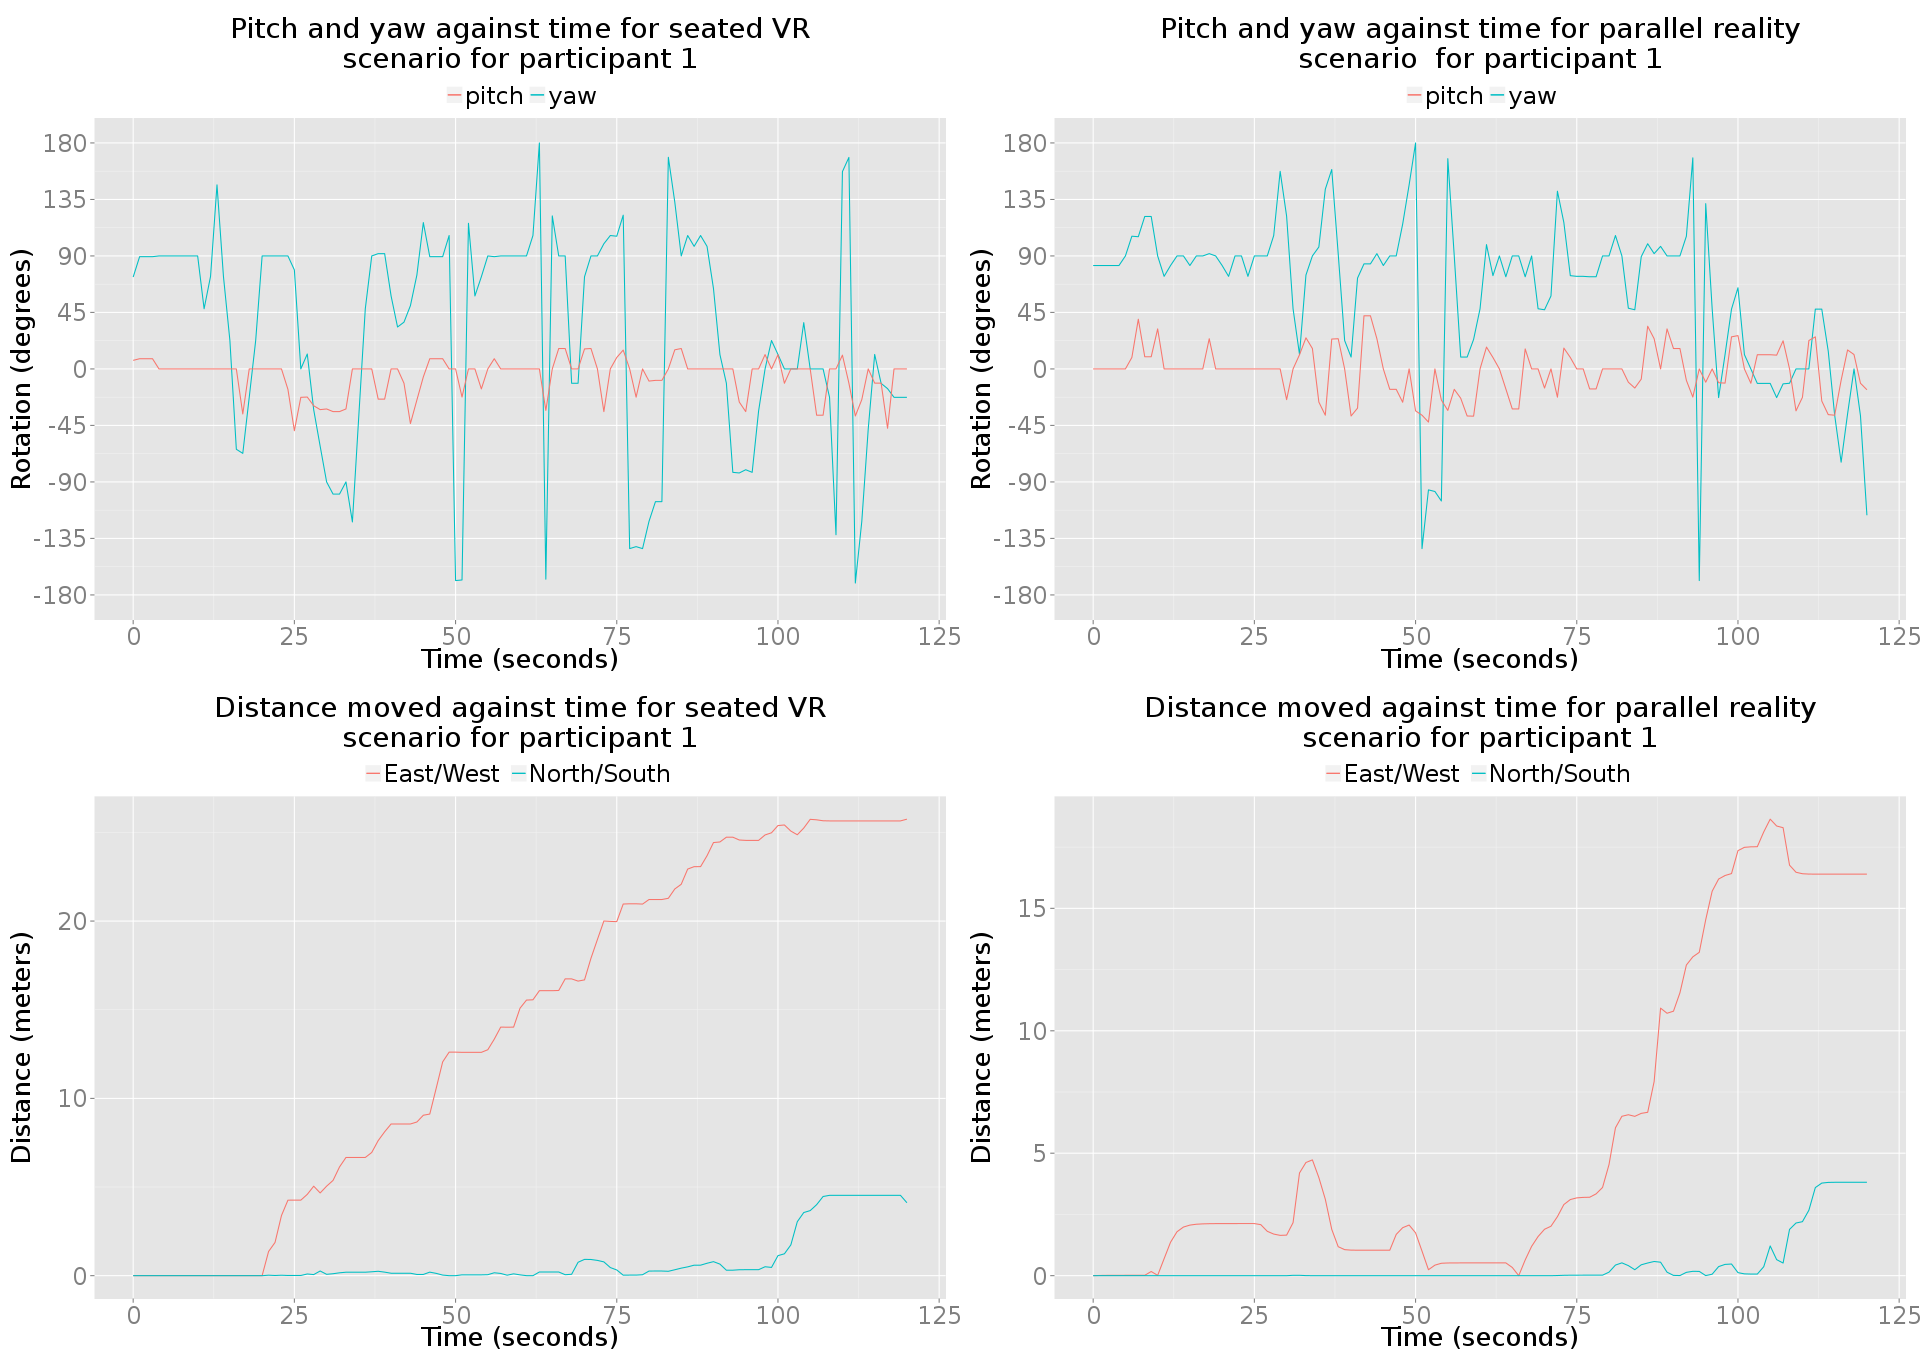
\includegraphics[width=\textwidth]{1/1_4up.png}
	\caption{Pitch and yaw against time, aligned with distance moved against time, for participant 1 in both scenarios.}
	\label{1_4up.png}
	\end{center}
\end{figure}

\begin{figure}
	\begin{center}
	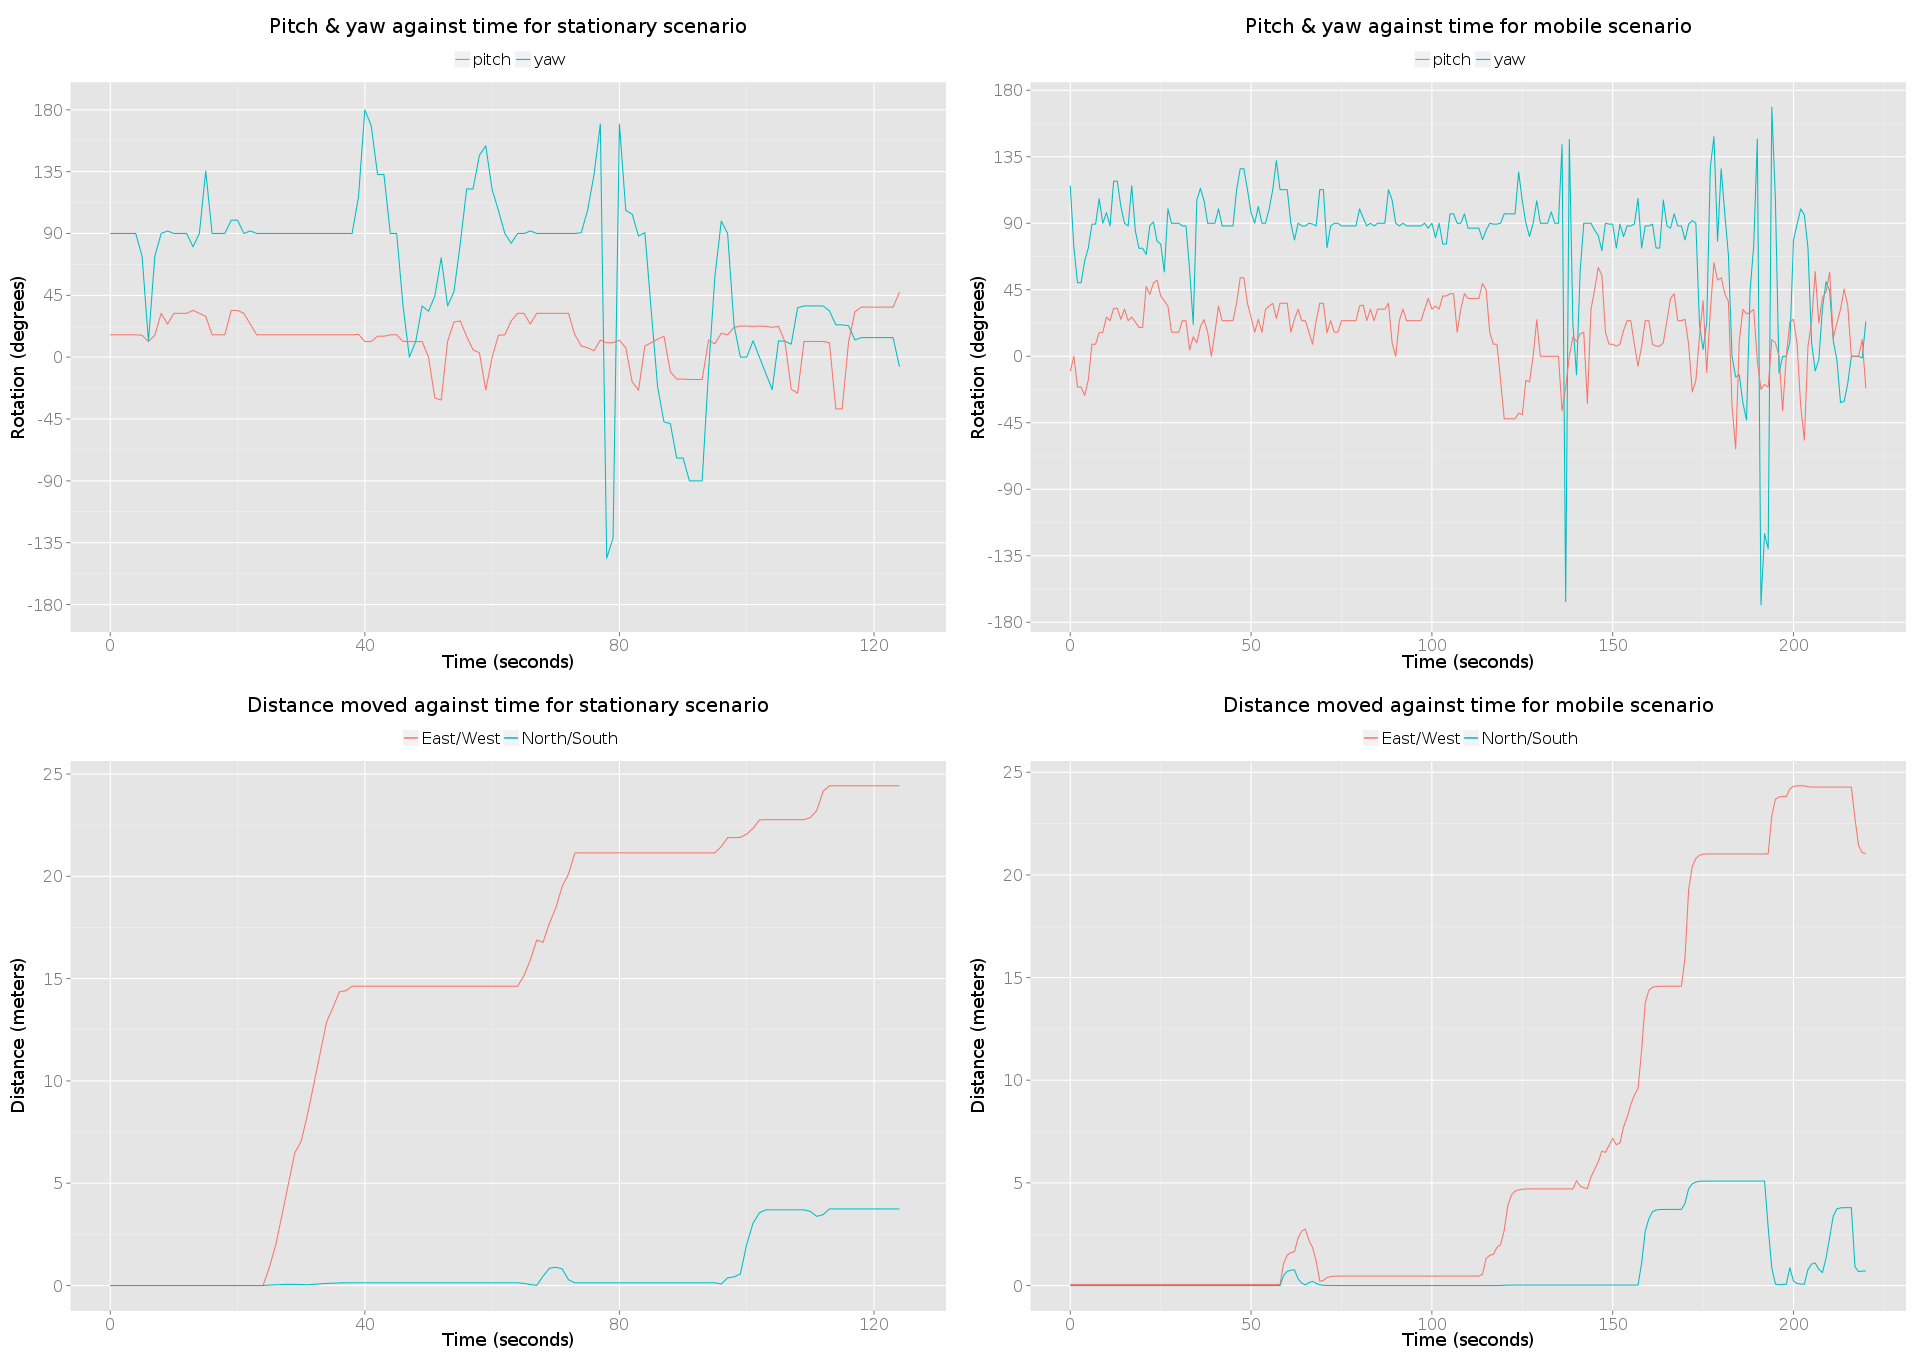
\includegraphics[width=\textwidth]{1/3_4up.png}
	\caption{Pitch and yaw against time, aligned with distance moved against time, for participant 3 in both scenarios.}
	\label{3_4up.png}
	\end{center}
\end{figure}

%=====================

\clearpage

Plotting position data upon the floorplan of the chapel reveal that several participants walked noticeably closer to the altar (far right of the floorplan) during the parallel reality scenario than during the VR section of the seated VR scenario. Figures \ref{06-seatedmap.png} (seated VR scenario) and \ref{06-movmap.png} (parallel reality scenario) show this relationship using participant 6 as an example. The reason for this is not immediately clear; it could be that the real altar presented a more interesting object for observation than its virtual counterpart, so that during the parallel reality scenario in which the real altar was visible participants found themselves drawn to it more than in the VR section of the seated VR scenario when only its virtual partner was visible, or it could be that participants who were less accustomed with the control methodology of the seated VR scenario simply wanted to complete the route as quickly as possible and thus took a more direct route to the `goal'.

\TwoFig{splodge-maps/06-seatedmap.png}{Position data (red dots) during VR section of seated VR scenario for participant 6.}{06-seatedmap.png}
       {splodge-maps/06-movmap.png}{Position data (red dots) during parallel reality scenario for participant 6.}{06-movmap.png}

%=====================

\subsubsection{Comparing RW and VR periods within parallel reality scenario}

When comparing head pitch and yaw data between the RW and VR periods within the parallel reality scenario, it is notable that for some participants there was more variance during the periods in which they were perceiving VR stimuli than during those in which they were perceiving RW stimuli, meaning that they turned their heads more when looking at the VR environment than when looking at the RW environment. This is particularly evident when plotting these pitch and yaw data against time with the periods of RW/VR indicated. Figure \ref{1_pitch_yaw.png} shows the head pitch and yaw data for participant 1 during the parallel reality scenario as an example of a participant who prominently displayed this tendency. The coloured background of the plot indicates which environment the participant was perceiving at that time index; blue for RW and green for VR. Correlation is evident between maximum variance in yaw and the periods that the participant was observing VR stimuli. As can be seen in figure \ref{3_pitch_yaw.png} this trend is even more prevalent in the data from participant 3, while the data from participant 5 in figure \ref{5_pitch_yaw.png} still show the trend but to a lesser extent.

\begin{figure}
	\begin{center}
	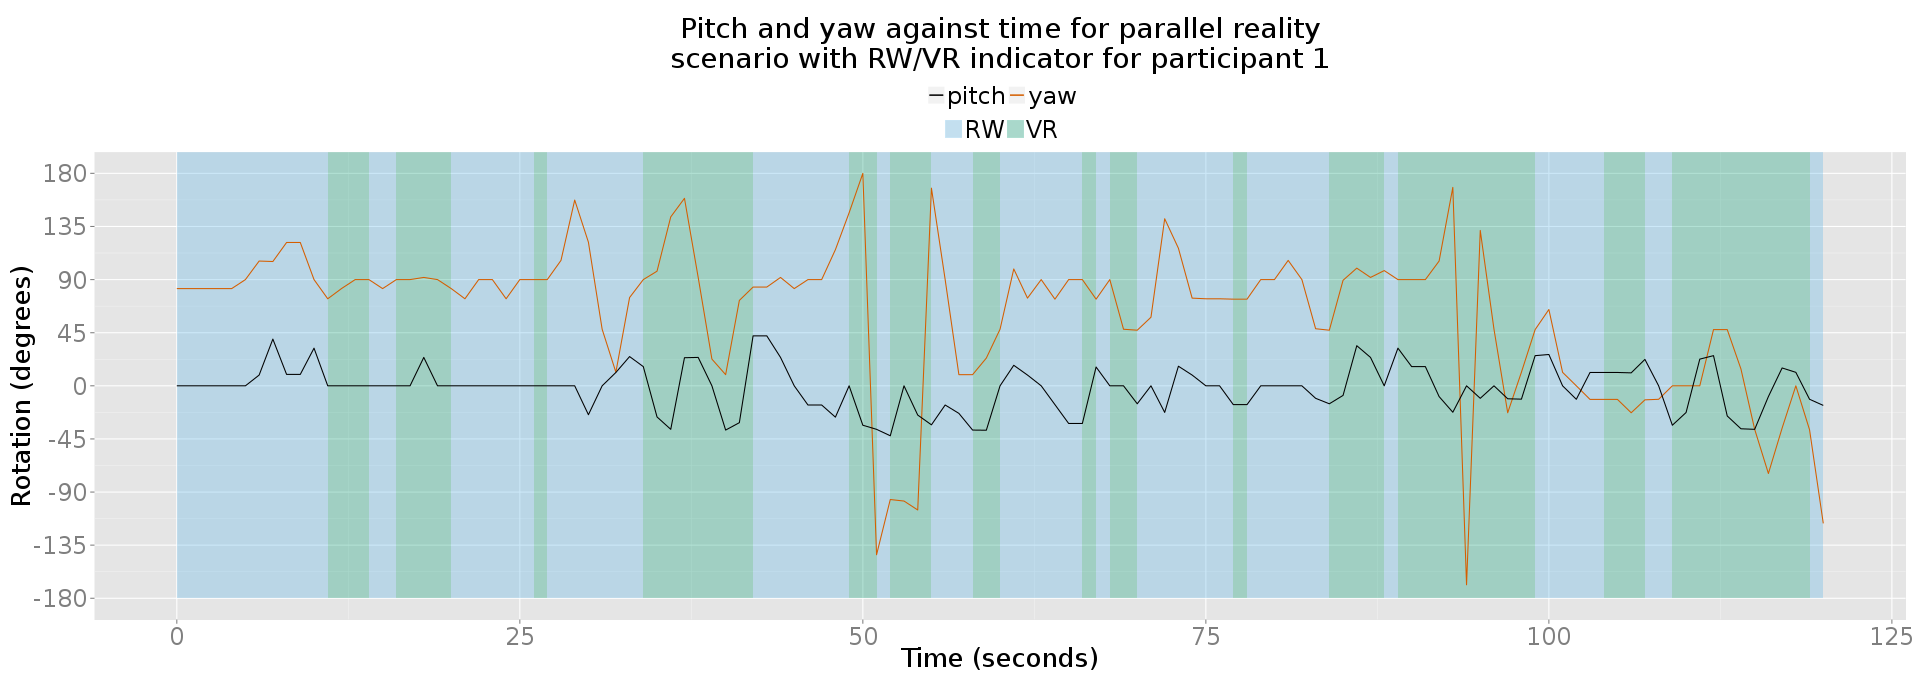
\includegraphics[width=\textwidth]{1/1_pitch_yaw.png}
	\caption{Pitch and yaw against time for participant 1 in parallel reality scenario, showing RW/VR periods.}
	\label{1_pitch_yaw.png}
	\end{center}
\end{figure}

\begin{figure}
	\begin{center}
	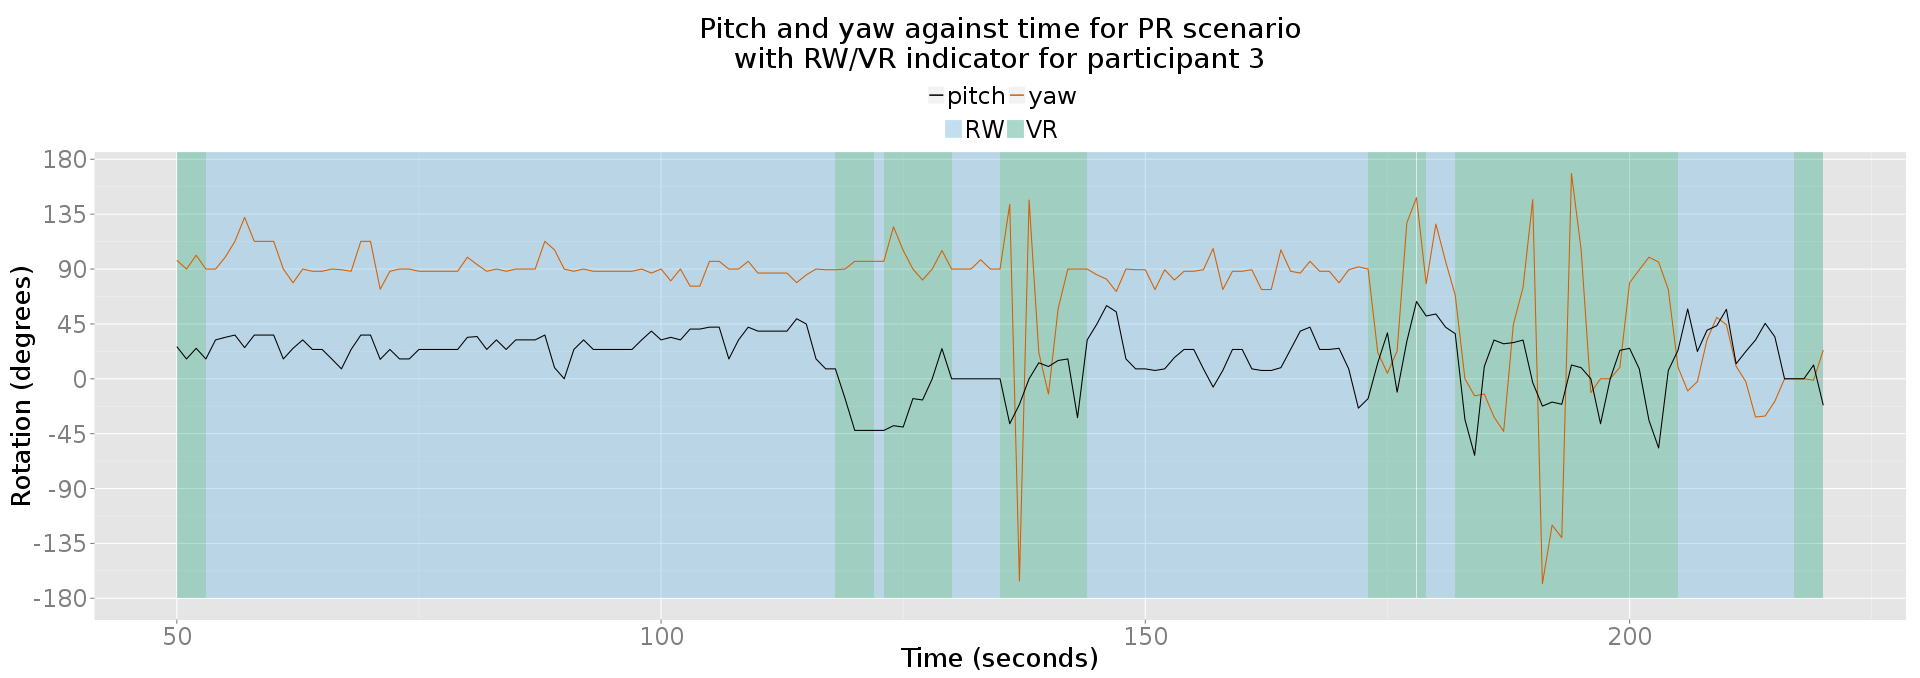
\includegraphics[width=\textwidth]{1/3_pitch_yaw.png}
	\caption{Pitch and yaw against time for participant 3 in parallel reality scenario, showing RW/VR periods.}
	\label{3_pitch_yaw.png}
	\end{center}
\end{figure}

\begin{figure}
	\begin{center}
	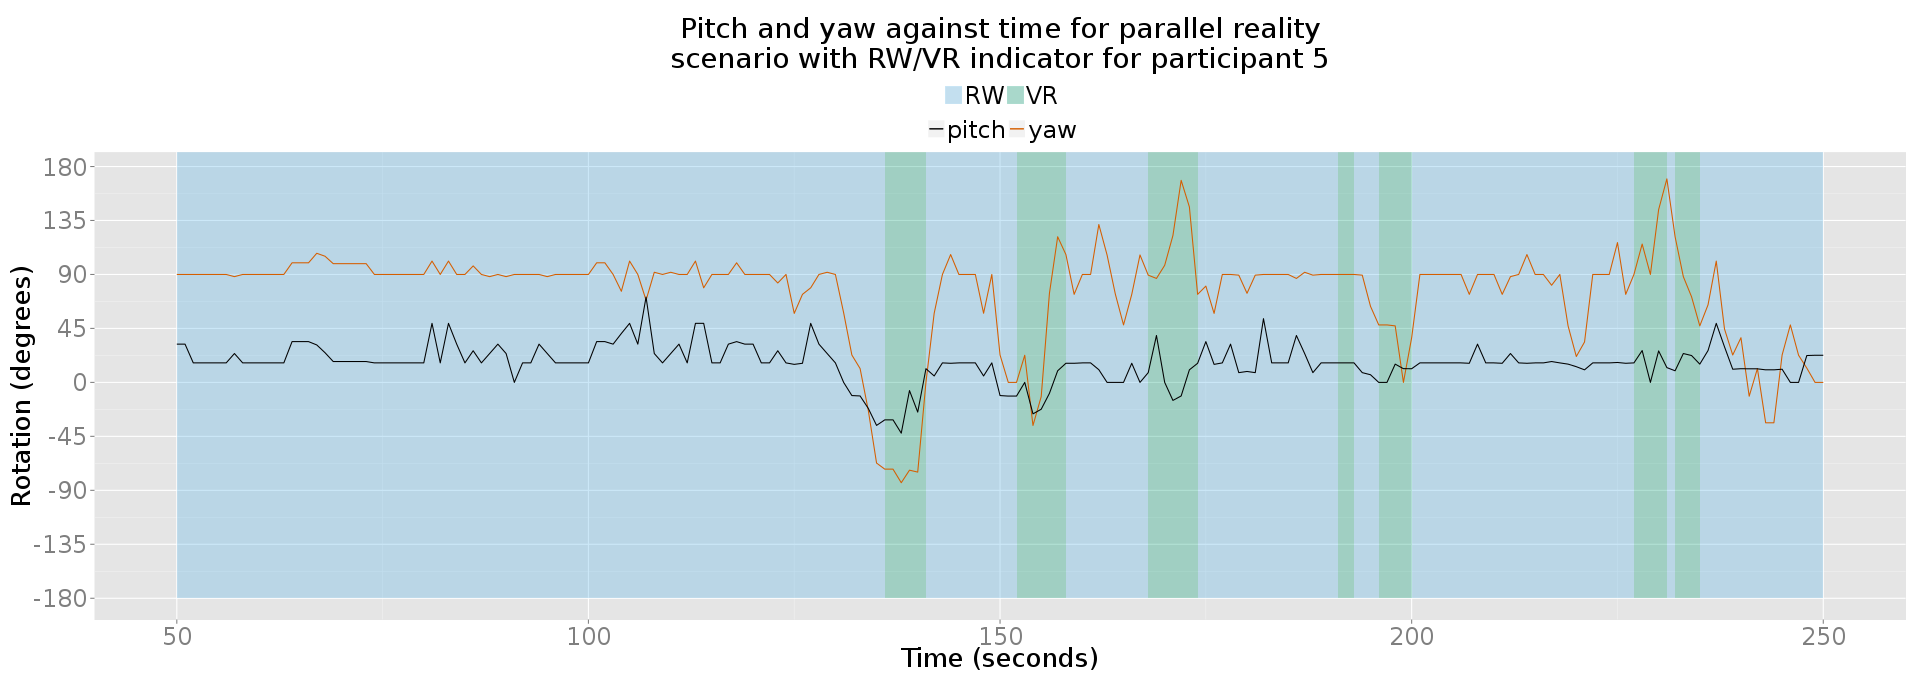
\includegraphics[width=\textwidth]{1/5_pitch_yaw.png}
	\caption{Pitch and yaw against time for participant 5 in parallel reality scenario, showing RW/VR periods.}
	\label{5_pitch_yaw.png}
	\end{center}
\end{figure}

\begin{table}
\begin{center}
\begin{minipage}[t]{.45\linewidth}
\begin{center}
\begin{tabularx}{\textwidth}{c *{3}{>{\centering\arraybackslash}X}}
\toprule

\textbf{Participant} & \textbf{RW (\textdegree)} & \textbf{VR (\textdegree)} \\

\midrule

1 & 13.325 & 17.554 \\

3 & 12.194 & 24.662 \\

4 & 6.133 & 8.837 \\

5 & 12.193 & 12.797 \\

6 & 15.712 & 15.349 \\

\bottomrule
\end{tabularx}
\caption{Weighted mean sd in pitch for parallel reality scenario.}
\label{sdpitchtab}
\end{center}
\end{minipage}
%
\begin{minipage}[t]{.02\linewidth}
\hfill%
\end{minipage}
%
\begin{minipage}[t]{.45\linewidth}
\begin{center}
\begin{tabularx}{\textwidth}{c *{3}{>{\centering\arraybackslash}X}}
\toprule

\textbf{Participant} & \textbf{RW (\textdegree)} & \textbf{VR (\textdegree)} \\

\midrule

1 & 25.545 & 39.887 \\

3 & 11.702 & 60.636 \\

4 & 18.032 & 15.300 \\

5 & 23.155 & 29.274 \\

6 & 41.717 & 47.440 \\

\bottomrule
\end{tabularx}
\caption{Weighted mean sd in yaw for parallel reality scenario.}
\label{sdyawtab}
\end{center}
\end{minipage}
\end{center}
\end{table}

\newpage

Calculating the mean standard deviation in yaw for both RW and VR periods, weighted by the duration of those periods, shows this relationship more analytically. With reference to the figures in table \ref{sdyawtab} the mean standard deviation in yaw while perceiving VR stimuli is higher than while perceiving RW stimuli for participant 1 (39.887\textdegree\ compared to 25.545\textdegree) and even more so for participant 3 (60.636\textdegree\ compared to 11.702\textdegree). The values are closer for participant 5 due to the initial large delta in yaw just before the first transition into VR at around 130 seconds. Recalculating the weighted mean standard deviation from 150 seconds onwards for participant 5 to exclude this peak gives rise to the values of 36.074\textdegree\ for VR stimuli compared to 17.046\textdegree\ for RW stimuli, which is more in fitting with the trend shown by figure \ref{5_pitch_yaw.png}. The exception to this observation of correlation between head movement and environment is participant 4, however this participant displayed very restricted head movement throughout both scenarios when compared to all of the other participants.

When considering the amount of time spent perceiving each environment in the parallel reality scenario, several of the participants showed frequent transitioning behaviour where they would perform many transitions and remain perceiving the visual stimuli from each environment for only a few seconds: for participants 1, 4 and 6, the mean times for both RW and VR periods are all between 1.68 and 3.4 seconds. Participant 3 spent longer perceiving each environment with a RW mean of 18.2 seconds and a VR mean of 7 seconds. The outlier is participant 5 with a RW mean of 31.8 seconds and a VR mean of 3.6 seconds; this was the participant who found it uncomfortable to walk while wearing the DK1, so a much longer amount of time spent perceiving RW stimuli is understandable.

\subsubsection{Comparing VR periods of parallel reality scenario to VR section of seated VR scenario}

Comparing head yaw during the VR periods of the parallel reality scenario (table \ref{sdyawtab}) against that from the VR section of the seated VR scenario (table \ref{sdpitchyawtrad}) shows that in most cases there is noticeably lower variance during the VR periods of the parallel reality scenario than in the seated VR scenario. This indicates that participants felt more comfortable to perform larger head movements when observing VR during the seated VR scenario than during the parallel reality scenario. Observations of participants while they performed the seated VR scenario support this conclusion, with several participants twisting their heads right around to look behind them without changing the direction of their virtual `movement'. During the parallel reality scenario participants tended to largely look ahead in the direction their body was facing, only turning their heads a large amount when turning their whole body around to begin walking in the return direction. As participants were restricted from reorienting their physical body during the seated VR scenario (the chair did not swivel) and several of them mentioned disliking the experience of using the controller to turn their virtual body whilst their physical body remained in the same orientation upon the chair (see section \ref{stage1interviews}), it is not surprising to see these larger changes in head orientation being employed to view all angles of the VR environment when seated.

Further comparing head movements between the seated VR scenario and the VR periods of the parallel reality scenario, the difference between the magnitude of pitch and yaw is greater in the seated VR scenario than in the parallel reality scenario. Comparing these values from tables \ref{sdpitchyawtrad}, \ref{sdpitchtab} and \ref{sdyawtab}, this difference exhibits as smaller variance in yaw and roughly unchanged (only slightly increased) variance in pitch for the VR periods of the parallel reality scenario, further indicating that participants were more comfortable or felt it more necessary to look around themselves more in the seated VR scenario than in the parallel reality scenario, leading to less overall head movement in the parallel reality scenario than the seated VR scenario.

%=========================================================================================================

\subsection{Graphical Performance}
\label{stage-1-framerates}
The overhead of capturing, processing and rendering the camera streams resulted in an overall lower framerate throughout the parallel reality scenario than the seated VR scenario, as shown by figure \ref{framerates_1.png}. Across all participants the seated VR scenario averaged 52.4 fps compared to 39.2 fps for the parallel reality scenario, representing a 25.2\% slowdown. Note that the refresh rate of the DK1 is 60Hz and the Mirrorshades Unity application was run with vsync enabled; vsync limits framerate to the refresh rate of the display to avoid screen tearing, so any values shown above 60 fps in figures \ref{framerates_1.png} and \ref{1-frames-2-up.png} are due to the method used to estimate fps.

\begin{figure}[ht]
	\begin{center}
		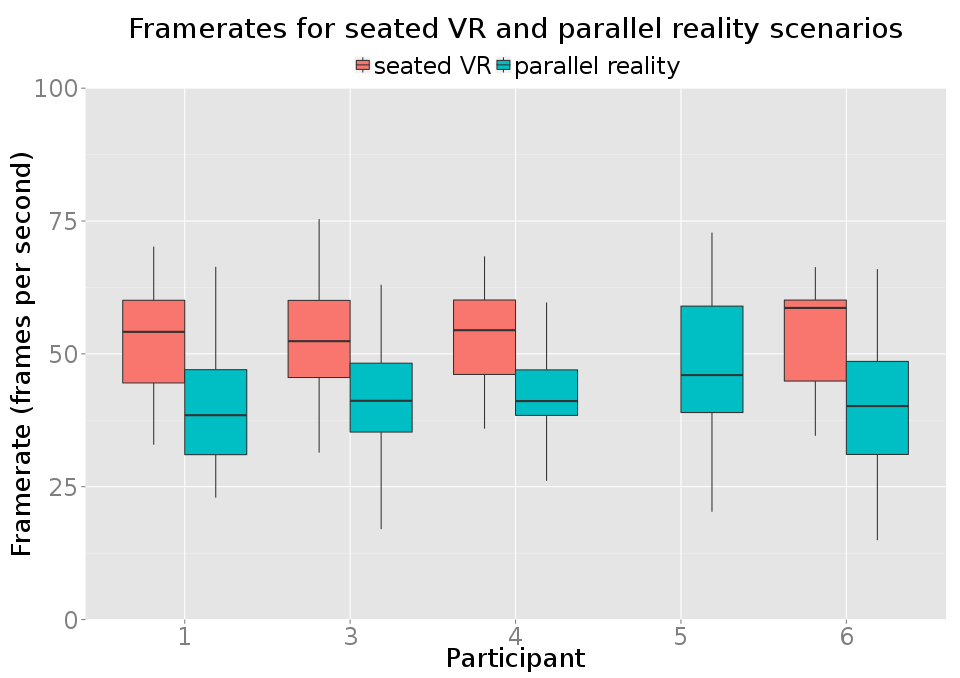
\includegraphics[width=.6\linewidth]{1/framerates_1.png}
		\caption{Framerates for both seated VR and parallel reality scenarios for all participants.}
		\label{framerates_1.png}
	\end{center}
\end{figure}

In the parallel reality scenario there was no real correlation between framerates and transitions between RW and VR stimuli, as can be seen in figure \ref{1-frames-2-up.png} (right) using participant 1 as an example that is representative of all participants in this stage. This is presumably due to the manner in which the RW and VR graphics are processed. The way that the culling masks used to obscure RW visuals when observing VR visuals and vice-versa are implemented in Unity did not seem to completely prevent the application from processing these unseen visuals. If this were the case, we would have expected to have seen framerate increase drastically during RW periods, as the rendering overhead of the camera streams should intuitively be much less than that of rendering the 3D environment of the VR chapel, however this relation was not exhibited.

\begin{figure}[ht]
	\begin{center}
		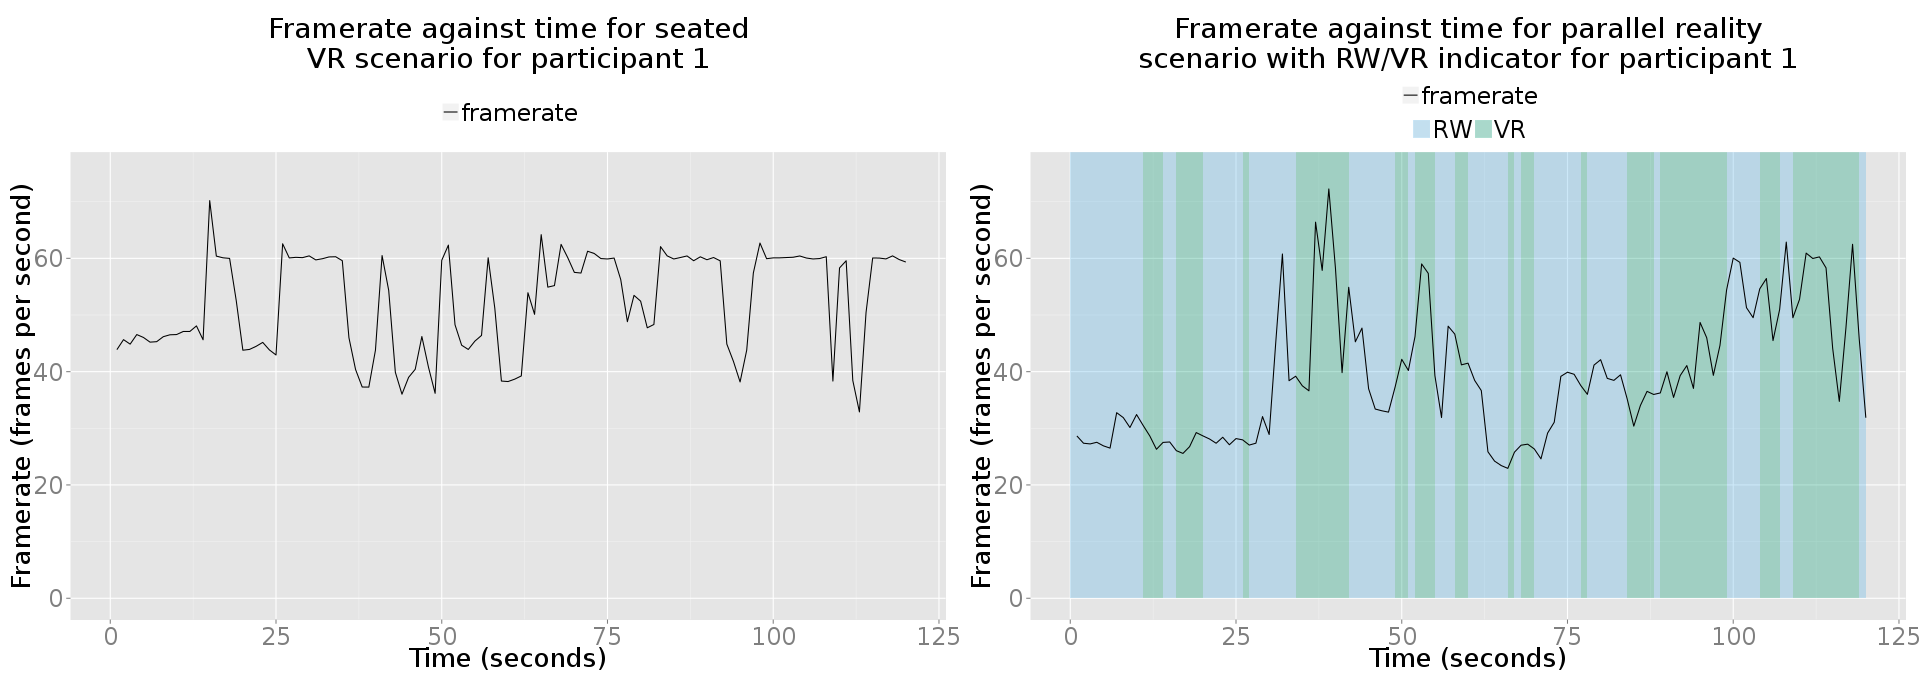
\includegraphics[width=\linewidth]{1/1-frames-2-up.png}
		\caption{Framerate against time for seated VR scenario (left) and parallel reality scenario (right) for participant 1.}
		\label{1-frames-2-up.png}
	\end{center}
\end{figure}

\newpage

Instead of varying according to whether the participant was observing RW or VR, the variance in framerate in the parallel reality scenarios instead varies more in accordance to what part of the chapel the participant was directing their view toward and whether they were moving or standing still. Certain parts of the 3D model are substantially more complex in terms of the number of virtual objects (and thus the number of draw calls required) and rendering moving graphics has an overhead compared to rendering a static scene. Comparing the parallel reality plot from figure \ref{1-frames-2-up.png} (right) to the plot of distance moved against time for the same participant in figure \ref{1_4up.png} (bottom right) hints at this relationship. The seated VR scenario plot (figure \ref{1-frames-2-up.png} left) shows periods in which framerate reached and was capped at the 60fps enforced by vsync.

%=========================================================================================================

\subsection{IndoorAtlas Performance}

Interview transcripts and video recordings of participants completing the parallel reality scenario indicate that the accuracy of the IndoorAtlas position data were largely perceived as being very good, with the lag in the data and the occasional large movement emerging as the stand out negative aspects of it.

Considering these occasional large movements, figure \ref{1-positiondeltas.png} shows the distance between subsequent IndoorAtlas positions for all participants throughout this stage of the user studies. Comparing this figure against figure \ref{vtwpositiondeltas.png} from the VTW evaluation immediately reveals how much better IndoorAtlas performed in this regard compared to both GPS receivers used in the VTW evaluation. The vast majority of position data were less than 1m from the previously reported position, which means that large movements in virtual position were rare. Furthermore, unlike with VTW where the GPS position data did not settle when the user stood still but instead continued to report different positions and thus continue to move the virtual vantage, IndoorAtlas was both accurate and fine grained enough to reliably recognise stationary periods. This is represented in figure \ref{1-positiondeltas.png} by the median for all participants being situated at or very close to 0 meters.

\begin{figure}[ht]
	\begin{center}
		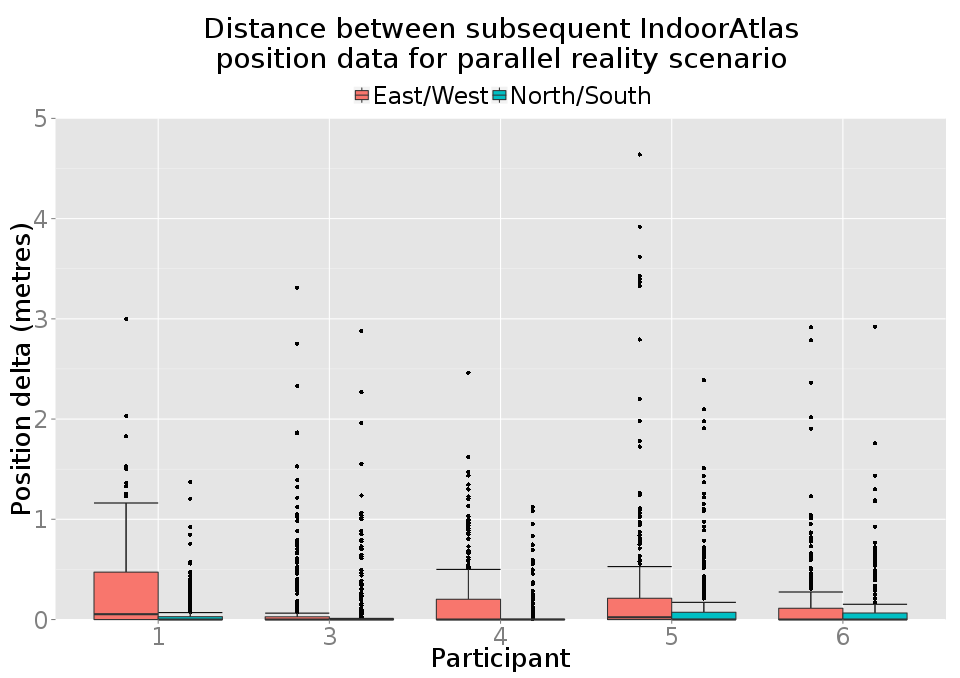
\includegraphics[width=.6\linewidth]{1/1-positiondeltas.png}
		\caption{Distance between subsequent IndoorAtlas position data.}
		\label{1-positiondeltas.png}
	\end{center}
\end{figure}

%=========================================================================================================

\subsection{Freeform Exploration and Detailed Comparison}

In terms of the three scenarios described in section \ref{parallel-reality-in-virtual-heritage} for application of parallel reality to virtual heritage, the Mirrorshades platform proved throughout this first stage of evaluation that it had both the positional accuracy and the orientational accuracy to fully achieve the freeform exploration scenario even in the confines of an indoor cultural heritage site and even when the participant is in very close proximity to walls/obstructions as shown in figures \ref{Mirrorshades-close-comparison-3.png} (participant viewing RW) and \ref{Mirrorshades-close-comparison-4.png} (participant viewing VR).

\TwoFig{Mirrorshades-close-comparison-3.png} {Mirrorshades functioning in close proximity to walls/obstacles (1/2).} {Mirrorshades-close-comparison-3.png}
       {Mirrorshades-close-comparison-4.png} {Mirrorshades functioning in close proximity to walls/obstacles (2/2).} {Mirrorshades-close-comparison-4.png}

Additionally the positional and orientational accuracy were for the most part even accurate enough for participants to perform detailed comparisons between real and virtual artefacts as close as arm's length, as shown in figures \ref{Mirrorshades-close-comparison-1.png} (participant viewing VR) and \ref{Mirrorshades-close-comparison-2.png} (participant viewing RW). These images are composites, with the participant's view through the HMD at the top left and a view of the participant themselves at the bottom right of each image.

\TwoFig{Mirrorshades-close-comparison-1.png} {Using Mirrorshades to perform detailed comparison between real and virtual artefacts (1/2)} {Mirrorshades-close-comparison-1.png}
       {Mirrorshades-close-comparison-2.png} {Using Mirrorshades to perform detailed comparison between real and virtual artefacts (2/2)} {Mirrorshades-close-comparison-2.png}

%=========================================================================================================

\section{Summary}

This first stage of evaluation directly compared a seated VR scenario, in which VR content has already come to be used at cultural heritage sites, against the mobile style of interaction afforded by the Mirrorshades parallel reality platform which addresses both temporal and spatial separation between experience of real and virtual environments. This evaluation has assessed the feasibility of the Mirrorshades platform with positive outcome and shown it to be a rewarding new modality for experiencing VR content in a cultural heritage context, improving upon seated VR techniques employed for the presentation of the same content, by allowing immediate comparison and contrast between corresponding vantage points in both the RW and VR environments, successfully addressing the hindrance of on-site comparison of real and virtual environments inherent to stationary virtual experiences.

The accuracy of position and orientation data throughout the evaluations was sufficient to fully realise the freeform exploration scenario from section \ref{parallel-reality-in-virtual-heritage} even in the confines of an indoor environment, and furthermore accuracy was for the most part sufficient for the freeform exploration with detailed comparison scenario. The immersive nature of the visuals produced by the Oculus Rift DK1 HMD, completely filling the user's FOV with stimuli from its screen, allowed for the experiential aspect of switching between real and virtual environments envisioned by the parallel reality paradigm to be truly accomplished by these scenarios.

Through questionnaire data and interview transcripts participants reported that overall they found the parallel reality scenario to be both more enjoyable and more rewarding than the seated VR scenario, despite the decreased usability and comfort effected by the requirement to don and carry a satchel of hardware and hold devices in both hands. The parallel reality scenario was reported as allowing easier comparison and contrast between RW and VR environments, leading participants to recognise more differences between the two environments and leading to greater learning and understanding of the chapel than with the seated VR scenario. Combined with reports of promoting greater awareness of both environments these responses indicate that the parallel reality scenario was successful in mitigating the vacancy problem.

Log data showed participants displaying restricted head movement throughout the parallel reality scenario, looking to their sides and above and beneath themselves less when experiencing the VR chapel in the parallel reality scenario than when experiencing the VR chapel in the seated VR scenario. While this restriction does not appear to have been so great that it reduced the utility and enjoyability of the parallel reality scenario to beneath that of the seated VR scenario, it has been observed by prior investigations~\cite{Slater1998} that there is a significant positive association between reported sense of presence in a VR environment and the amount of body movement, particularly head yaw, displayed by a participant. Furthermore, reducing the negative impact that a parallel reality system has upon a user's willingness to freely look around them will result in beneficial returns, especially when considering that restricted head movement may lead to overlooking interesting aspects of \textit{both} environments, not just the VR one.

Criticisms of the experience were primarily levelled at aspects of the system that were constrained by hardware limitations, rather than at conceptual aspects of the experience. The visual acuity of the RW environment afforded by the cameras during the parallel reality scenario, which was substantially poorer than participants' unmediated eyesight during the seated VR scenario, was one prominent complaint, while the lag of the IPS surfaced as a major detractor to enjoyment of the experience even though its accuracy was high.

%=========================================================================================================
%=========================================================================================================
%=========================================================================================================
%=========================================================================================================
%=========================================================================================================

%\clearpage

\chapter{Evaluation: Informed Parallel Reality}

%\section{Stage 2 - Informing Parallel Reality Implementation}

\begin{quote}
	\textit{``Let us wander in modernism's cabinet of curiously segmented senses to see what doors we might open to a differently mediated sensorium.''}
\end{quote}
\hfill \textit{The Mediated Sensorium, Caroline A. Jones}
\\
\\

%=========================================================================================================

\label{chapter-eval-2}

This chapter recounts the second stage of evaluation conducted with the Mirrorshades platform, in which the focus was upon investigating how certain aspects of the platform's implementation affected the overall parallel reality experience. A first user study compared different manners of transitioning between RW and VR visual stimuli, while a second investigated changes to the balance between RW and VR visuals in the default view. The results of these studies furthered the establishment of a set of best practices to inform future parallel reality endeavours.

%=========================================================================================================

\section{Overview}

Stage 2 of the evaluation comprised two parts. The first, stage 2.1, focussed upon assessing participants' reactions and preferences toward four different transition styles (the first aspect identified in section \ref{design-considerations-for-rw-vr-transitions}). The second, stage 2.2, looked at reactions and preferences in response to two different default views comprising RW/VR mixes (the second aspect identified in section \ref{design-considerations-for-rw-vr-transitions}).

In terms of the combined Milgram/Waterworh model these evaluations pertained to assessing the effect upon participants' focus of attention, assessing the severity of the break in presence in the terms of the extended vacancy problem, when performing oscillations along the locus of attention axis. Stage 2.1 investigated oscillations wherein the default view was 100\% RW, with participants performing oscillations using different transition implementations between the RW extreme of the locus of attention axis and other points upon it (such as in figure \ref{transition-rw-vr-hard.png}). Stage 2.2 looked at oscillations wherein the default view was a mix of RW and VR, limiting how far toward the RW extreme of the locus of attention axis the participant could reach (such as in figure \ref{transition-mix-vr.png}).

While stage 1 of the evaluation focussed primarily upon assessing the feasibility of the concept and its worth in a virtual heritage scenario, stage 2 has broader implications for informing implementation of future parallel reality systems in general.

\begin{figure}[ht]
	\begin{center}
		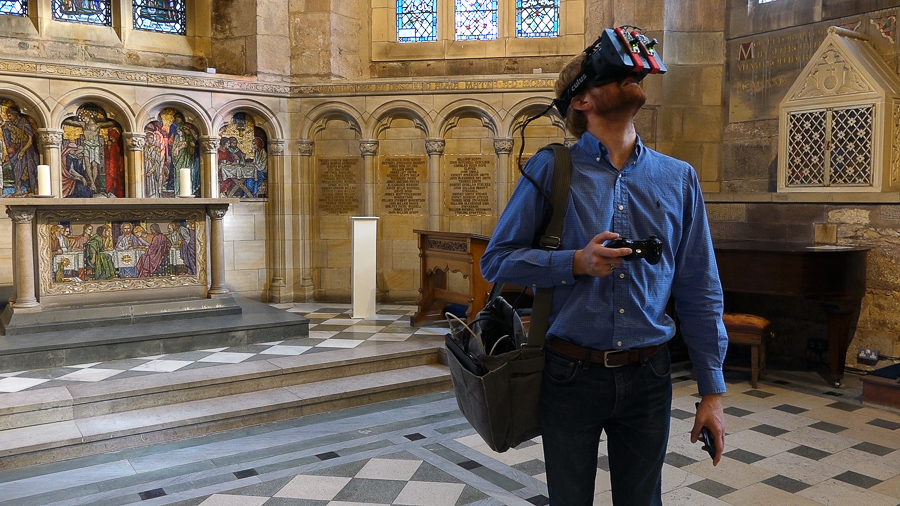
\includegraphics[width=\linewidth]{participant-m.jpg}
		\caption{Participant using Mirrorshades in a user study at St Salvator's chapel.}
		\label{participant-m.jpg}
	\end{center}
\end{figure}

%=========================================================================================================

\section{Evaluation Techniques}
\label{stage-2-1-evaluation-techniques}
As with the stage 1 evaluation a range of both qualitative and quantitative data were collected throughout both stage 2.1 and stage 2.2. Evaluating participants' preferences toward different styles of transitioning between RW and VR visual stimuli pertains to studying their reactions and responses to ascertain the effect upon their focus of attention, a concept that is largely psychological in nature (\textit{``Psychology is the physics of virtual reality''}\footnote{\url{ftp://ftp.hitl.washington.edu/pub/publications/papers/m-90-1.html}}) and highly subjective~\cite{Ijsselsteijn2001}. Subjective measures thus produced the bulk of the data for evaluation, however they were once again backed up by objective log data to support or contradict emerging relationships.

Stage 2 participants completed the same pre-task questionnaire as stage 1 participants and Likert-type questionnaires that shared certain items with that from stage 1 were also used; the stage 2.1 participants completed a 12-item questionnaire (included as appendix \ref{appendix-12-item-likert-type-questionnaire-stage-2-1}), while stage 2.2 participants completed a 9-item questionnaire (included as appendix \ref{appendix-9-item-likert-type-questionnaire-stage-2-2}). The SUS questionnaire was not used, while post-task interviews (prompts included as appendices \ref{appendix-interview-questions-stage-2-1} and \ref{appendix-interview-questions-stage-2-2} for stages 2.1 and 2.2 respectively) and logging were present. ShadowPlay was used to record the visuals displayed upon the DK1 and video cameras were used to record the participants themselves. Additionally, all stage 2 participants also completed the igroup presence questionnaire (see section \ref{igroup-presence-questionnaire-explanation}).

As presence does not have a single widely agreed upon definition and those definitions that are commonly used are subjective in nature due to the fact that presence (whether in physical or virtual environments) is perceptual~\cite{Waterworth2014}, attempts to quantify or `measure' the experience of presence are met with difficulty. Many different approaches have been adopted, some of which are more or less suitable to certain scenarios than others. These approaches can be broadly categorised as either subjective (most commonly post task questionnaires), behavioural (measurement/observation of actions that do not stem from conscious thought) or physiological (heart rate, skin conductance, etc.)~\cite{Insko2003}.

Under these categories one can consider the log data recorded by the Mirrorshades platform to provide a behavioural insight into the participants' sense of presence and the interview and Likert-type questionnaires to provide a subjective insight. Because this second stage of evaluation elicited direct comparisons between different styles of transition, in hopes of ascertaining which resulted in less pronounced breaks in presence due to the extended vacancy problem, the use of an established presence questionnaire was deemed a prudent addition to the evaluation techniques in order to inquire more directly about this aspect of the experience and to do so in a standardised fashion.

%=========================================================================================================

\subsection{Presence Questionnaires}
\label{presence-questionnaires}
Due to the nature of the Mirrorshades platform and the adoption of the break in presence definition as held by Waterworth and Waterworth and the extended vacancy problem, most established presence questionnaires could not be directly applied. These presence questionnaires have predominantly been written for application to `full immersion' VR scenarios in which the user is immersed in a VR (or remote, in the case of telepresence) environment at the intentional exclusion of stimuli from their RW environment, adopting the Slater and Steed model of the break in (virtual) presence concept, upholding the notion of \textit{``VR as portal to a private world of simulation where physical senses are immersed by prosthetics, where users temporarily `forget' their primary sensory world''}~\cite{Heim2014}.

Illustrated in reference to an embodied cognition framework, as for mediated presence \textit{``action is more important than perception''}~\cite{Giuseppe2014}, the sense of presence in these full immersion VR scenarios is argued to develop from the construction of a spatial-functional mental model of the VR environment. This is achieved by the representation of bodily actions as being possible in the VR environment in combination with suppression of incompatible sensory input from the RW environment~\cite{Schubert2001}. A break in presence can result here from a mismatch between the predicted state of a virtual object using a motor representation and the actual state of the object after enacting that motor representation~\cite{Giuseppe2014}.

However considering a parallel reality scenario within the same framework, sensory input from a RW environment that features high spatial equivalence and an equivalent vantage point with the VR environment is not incompatible, but instead complimentary and we do not wish for the user to `forget' about either `sensory world'. Whereas a full immersion VR experience attempts to create in the user's mind a new spatial-functional model that exists separate to, likely incompatible with and requiring suppression of the model of their RW surroundings, parallel reality systems should instead be considered as enhancing the user's existing model of their RW surroundings, or alternatively as creating a complementary model that sits parallel to the RW model and can be attended to in tandem. The effect of this complimentary nature of the environments can be considered within the context of Waterworth and Waterworth's `three layers of presence'~\cite{Mantovani2010, Giuseppe2014} that constitute:

\begin{enumerate}

\item \textbf{Proprioceptive or `proto' presence}, which is concerned with the correct coupling of perceptions and movements, with high proprioception-action coupling leading to heightened embodied presence.

\item \textbf{Perceptual or `core' presence}, as the ability of a subject to identify the external world and its current tasks in that world as separate from the self.

\item \textbf{Reflective or `extended' presence}, as the ability of a subject to verify to itself the significance of experienced events in the external world and which leads to the ability to experience absence, situated at the extreme of the focus of attention axis opposite presence.

\end{enumerate}

Each of these three levels is associated with one of Damasio's evolutionary levels of selfhood~\cite{Damasio1999} and the Waterworths' reasoning leads to the position that:

\begin{quote}
\textit{``Presence is maximised when all three layers are integrated around the same external situation, whether this is physical reality, virtual reality, or a mixture of the two.''}~\cite{Mantovani2010}
\end{quote}

While RW experiences rarely feature conflict between the proto-presence and core presence layers, VR experiences often present such conflict due to mismatch between physical actions and perceived (virtual) results owing to the conflicting content of the two environments. A parallel reality system whose two constituent environments share high spatial equivalence however, should not present such a mismatch between proto- and core presence layers.

The implication this has upon the suitability of established presence questionnaires to parallel reality platforms is perhaps best illustrated by appreciation of the lack of consensus when it comes to the definition of the term `presence'~\cite{Calleja2014} (and thus `break in presence'), with many questionnaire authors using the term to mean only mediated presence~\cite{Mantovani2010} and \textit{``to refer to experiencing a purely VR as if it were a real place''}~\cite{Steed2014}\footnote{More precisely many use the term to mean only \textit{virtual presence}, defined in this context as a subset of mediated presence that is interested only in those experiences of `being in' a virtual environment and not, for example, experiences of `being in' a remote real environment as is the case with telepresence.}. Visualised using the combined Milgram/Waterworth model, established presence questionnaires in this vein largely assess presence in terms of the user's position upon the locus of attention axis, where `a sense of presence' construes a position toward the VR extreme of the axis and `no sense of presence' means a position toward the RW extreme of the axis. A break in presence in this context is that of the Slater and Steed definition (see discussion in section \ref{background-breaks-in-presence}) as a shift upon the locus of attention axis from VR to RW.

In this stage of the evaluation into the Mirrorshades parallel reality platform however, the aim was to assess presence in terms of the user's position upon the focus of attention axis, to assess the severity of breaks in presence considered under the Waterworth and Waterworth and extended vacancy problem definition as deflections upon the focus of attention axis from the presence extreme in the direction of the absence extreme, representing increased cognitive load caused by performing a transition between two environments. Instead of assessing allocation of locus of attention between two \textit{incompatible} sets of environmental stimuli, this stage of evaluation studied the impact that a locus of attention oscillating between \textit{complimentary} sets of environmental stimuli had upon the participant's focus of attention.

Thus instead of issuing a questionnaire designed to determine the balance between virtual presence and real presence, this evaluation needed to employ a questionnaire that provided insight into the balance between presence (whether real or virtual) and absence. Many established presence questionnaires that feature wording and weighting of questions associating negativity to awareness of the stimuli from the RW environment were thus unsuitable. Whilst this approach is ideal for a full immersion VR scenario in which awareness of the VR environment at the complete exclusion of the RW environment is the ultimate goal, it does not apply well to a parallel reality scenario in which the ultimate goal is to imbue the user with the ability (and desire) to freely transition between both RW and VR environments, wherein maintaining an awareness of one environment while perceiving stimuli from the other is beneficial, rather than detrimental, to the overall experience.

Witmer and Singer's presence questionnaire~\cite{Witmer1998} for example, poses several questions that directly enquire about aspects of the virtual environment (\textit{``13. How involved were you in the virtual environment experience?''}) but poses no questions that pertain to the RW environment other than a single comparison between VR and RW (\textit{``7. How much did your experiences in the virtual environment seem consistent with your real world experiences?''}, an assessment touching on perceived realism and of how well bodily actions were represented as possible in the VR environment). Other questionnaires such as that from Slater and Steed, in which participants walked through a VR field of trees~\cite{Slater1998}, are less extreme in their weighting toward questions only about VR, asking questions about the VR environment (\textit{``Please rate your sense of being in the field among the plants''}) but also enquiring as to the sense of being in the RW environment in a neutral tone (\textit{``During the time of the experience, which was strongest on the whole, your sense of being in the virtual field, or of being in the real world of the laboratory?''}). However even this permeates an `either or' implication to the two environments, emphasising their incompatibility and separateness.

%=========================================================================================================

\subsection{The Igroup Presence Questionnaire}
\label{igroup-presence-questionnaire-explanation}
The igroup presence questionnaire (IPQ, included as appendix \ref{appendix-igroup-presence-questionnaire})~\cite{Schubert2001} assesses presence based upon three factors: spatial presence (SP), involvement (INV) and realness (REAL). While SP questions assess how much bodily actions are represented as possible in the VR environment and REAL questions assess the perceived `realness' of the VR environment by eliciting direct comparisons with the RW environment, INV questions assess suppression of sensory input from the RW environment. However INV questions are worded in a manner that does not associate attention paid to this RW sensory input as inherently negative, or even such that these stimuli are considered incompatible, reducing risk of negative bias when the questionnaire is applied to a scenario in which attention paid to RW stimuli is encouraged, such as an application of parallel reality.

For a well implemented full immersion VR experience that elicits a high sense of virtual presence in the user, one would expect their IPQ results to score highly in all three factors. As discussed by Constantin~\cite{Constantin2003}, SP3 (\textit{``I did not feel present in the virtual space''}, anchored between \textit{``did not feel''} and \textit{``felt present''}) and INV2 (\textit{``I was not aware of my real environment''}, anchored between \textit{``fully disagree''} and \textit{``fully agree''}) would even seem to be fairly directly tied together, as a high involvement in the RW environment would intuitively reduce spatial presence in the VR environment by hampering the sense that bodily actions are possible there. The vacancy problem that effects this style of VR experience would be demonstrated upon IPQ results as a reduction in INV scores (greater awareness of the real environment) causing a reduction of similar magnitude in SP scores (less experienced presence in the virtual space).

In a parallel reality scenario that features high spatial equivalence between its constituent RW and VR environments, this tie between SP and INV was not expected to demonstrate so strongly. Due to the spatial equivalence between the two environments and the fact that the user's view of the virtual is of the equivalent vantage, bodily actions in the VR environment are inherently compatible with those in the RW environment - they could even be said to mimic or imitate them. Thus SP may score highly even when INV scores low, as RW sensory input isn't suppressed but in fact encouraged. It may even be the case that an inverse relationship presents between SP3 and INV2, as heightened awareness of the RW environment leads the user to a more believable representation of bodily actions in the VR environment as possible, increasing SP as RW bodily actions are shared (`possible') with the VR environment. Such a discrepancy between INV and SP scores for a parallel reality experience would demonstrate the ability of the concept to mitigate the extended vacancy problem that effects full immersion VR experiences where the scores remain more closely tied. In fact it would not be an inductive leap to interpret the magnitude of this discrepancy between INV and SP scores as a direct indication of how well the platform managed to mitigate the extended vacancy problem.

A conservative expectation for the results of the IPQ when applied to a parallel reality experience would be for generally lower INV scores than for a full immersion VR experience but without an accompanying drastic reduction in SP scores. An optimistic expectation for a well implemented parallel reality experience would be for lower INV scores and \textit{heightened} SP scores; that reinforcement of bodily actions within the RW environment lead to an increase in experienced spatial presence in the VR environment.

Although a traditional view of augmented reality is that it aims to enhance the sense of presence in the physical world~\cite{Waterworth2014}, this does not necessarily stand as an aim of parallel reality. This is due to the fact that instead of augmenting the primary environment of the user's RW surroundings, parallel reality instead presents the user with two separate (debatably both or alternatingly `primary') environments.

%=========================================================================================================

%there isn't really a mapping from SP/INV/REAL to focus/locus/sensus.
% INV kinda maps to locus & effects focus

% ***but why didn't we add physiological measures as well?

%=========================================================================================================

\section{Stage 2.1 - Evaluating Transition styles}

The stage 2.1 evaluation was conducted using a similar approach as that employed by stage 1. Participants first received a full immersion VR experience by using the DK1 and Xbox controller to explore the VR chapel while seated and subsequently completed the IPQ. This served both to acclimatize participants to the DK1 (in a similar vein as the use of the Tuscany demo in the stage 1 evaluation) and to produce baseline IPQ results for a full immersion VR experience of the chapel model using the DK1 with RW stimuli intentionally suppressed. Participants then performed two parallel reality scenarios in which they walked through the RW/VR chapels (see figure \ref{participant-m.jpg}) in a similar manner to the parallel reality scenario in stage 1, thus completing three scenarios in total:

\begin{enumerate}
	\item \textbf{Seated VR scenario} - Participants explored the VR chapel from a seated position, as VR has already come to be employed at cultural heritage sites via CAVE installations and by the OVW group with Oculus HMDs, using the Xbox controller to move around the VR environment observed via the DK1, with the DK1 obscuring their view of the RW chapel around them.
	\item \textbf{Parallel reality scenario with transitions 1-3} - (Referred to as `scenario 1-3') Participants experienced the RW and VR chapels in tandem using the Mirrorshades platform. They wore the DK1, held the Xbox controller in their right hand and the smartphone in their left, with the laptop and control box bundle in a satchel worn over a shoulder. The default view on the DK1 screen was 100\% RW and they were granted access to 3 different transition styles:
	\begin{enumerate}
		\item Hard transition (section \ref{sub-hardswitch}) mapped to controller \texttt{[A]} button (referred to as `transition 1').
		\item Transition with linear interpolation (section \ref{transition-with-linear-interpolation}) mapped to controller \texttt{[B]} button (referred to as `transition 2').
		\item Analogue selectable opacity (section \ref{analogue-selectable-opacity}) mapped to controller right trigger \texttt{[RT]} (referred to as `transition 3').
\end{enumerate}
	\item \textbf{Parallel reality scenario with transitions 1-4} - (Referred to as `scenario 1-4') Participants experienced the same scenario as scenario 2, however this time with the introduction of the periodic hard transition (section \ref{subsub-periodic}, referred to as `transition 4') which would trigger a 0.15 second transition to 100\% VR every 3 seconds. The 3 second timer was reset each time the user manually triggered a transition using any one of transitions 1-3.
\end{enumerate}

In the parallel reality scenario with transitions 1-3 pressing and holding the \texttt{[A]} button triggered a hard transition from 100\% RW to 100\% VR, pressing and holding the \texttt{[B]} button triggered a linear interpolated transition from 100\% RW to 100\% VR and pulling on the right trigger \texttt{[RT]} reduced the opacity of the game objects upon which the video see-through camera feeds were rendered from 100\% to an amount that mapped to the amount that the trigger was pulled. Pulling the trigger all the way in would reduce the opacity of the objects to 0\% and thus display 100\% VR, pulling the trigger 33\% would reduce the opacity of the objects by 33\% and thus display 66\% RW and 33\% VR, etc. In the parallel reality scenario with transitions 1-4 participants were granted access to the same 3 transitions via the Xbox controller and additionally the 4th transition of the periodic hard transition was triggered every 3 seconds for a duration of 0.15 seconds.

Rather than describing a path through the chapel with particular positions of interest to stop and look around at, participants were simply told to slowly make their way from the starting position at the West end of the chapel down to the altar at the East end of the chapel. During the stage 1 evaluation participants' exploration sometimes seemed to be restrained by their adherence to the described route. In order to promote a more natural style of exploration the use of a roughly described route was removed from the second stage of the evaluations.

%=========================================================================================================

\section{Stage 2.1 Results}

A total of 7 participants completed the stage 2.1 evaluation:
\begin{itemize}
	\item Age ranged from 18 to 27, with a mean of 22.3 and a standard deviation of 4.
	\item 5 identified as male and 2 as female.
	\item All reported previous experience with a games console controller.
	\item None reported previous experience with a HMD.
	\item 2 reported having previously visited the real world chapel.
	\item None reported having previously experienced the virtual chapel.
\end{itemize}

As with the stage 1 evaluation, the small sample size and range of ages involved in the stage 2.1 evaluation means that the observations drawn from these results should be considered in the same manner: as initial evidence that informs the high level best practices discussed in section \ref{best-practices-for-parallel-reality} and which justifies and informs more comprehensive future work, rather than as detailed claims to specifics of implementations or concepts. Original data can again be obtained by contacting the author\footnote{\texttt{cj@cjdavies.org}}.

%=========================================================================================================

\begin{figure}
	\begin{center}
	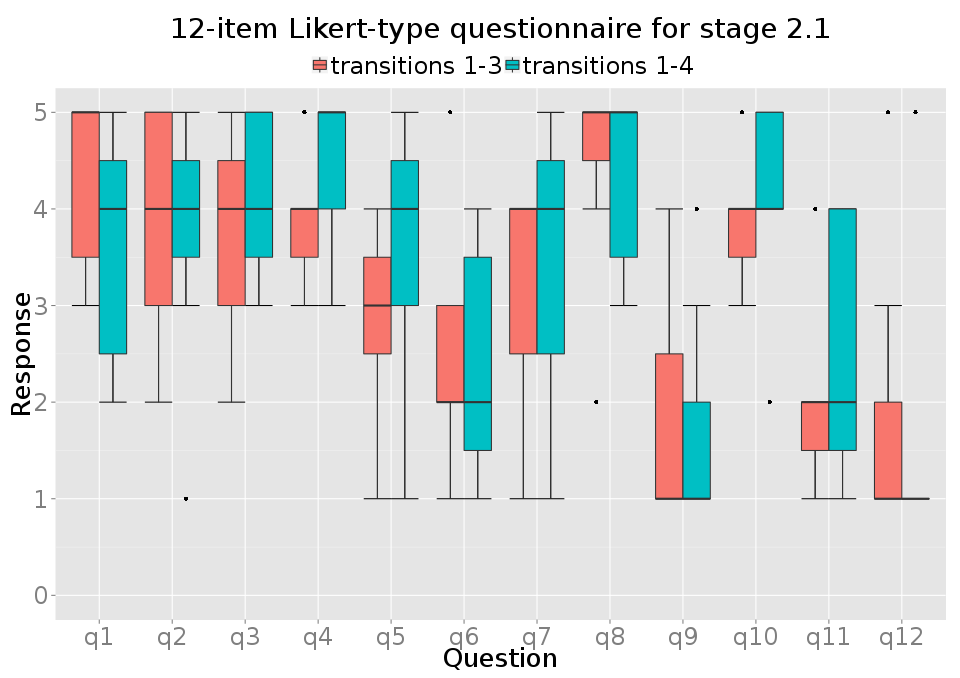
\includegraphics[width=.6\textwidth]{2.1/12-item-likert-type-questionnaire-boxplot.png}
	\caption{Stage 2.1 evaluation Likert-type questionnaire results.}
	\label{2-1-12-item-likert-type-questionnaire-boxplot.png}
	\end{center}
\end{figure}

%=========================================================================================================

\subsection{Likert-type Questionnaires}
The responses to the questionnaires are presented by figure \ref{2-1-12-item-likert-type-questionnaire-boxplot.png} with the questions reproduced below. All questions were answered on a scale from 1 to 5, anchored between `strongly disagree' and `strongly agree' respectively:
\begin{enumerate}
	\item I found the exploration an enjoyable experience.
	\item I preferred one transition more than the others.
	\item I was aware of both real and virtual environments.
	\item It was easy to compare features from the past and the present.
	\item I preferred different transitions in different situations.
	\item It felt as though I was in the past.
	\item I felt motion sickness/dizziness.
	\item It was rewarding to explore the chapel in this way.
	\item I forgot that there were different transitions available.
	\item I feel I now better understand what the chapel was like in the past.
	\item Switching between real and virtual was uncomfortable.
	\item I did not notice differences between the real and virtual environments.
\end{enumerate}

These responses indicate that participants overall found scenario 1-3 to be more enjoyable than scenario 1-4 (q1), although scenario 1-4 made them more aware of both environments than scenario 1-3 (q3) and allowed them to compare features from past and present more easily (q4), with participants not noticing differences slightly more in scenario 1-3 than in scenario 1-4 (q12). Participants reported preferring one transition over others in certain situations more in scenario 1-4 than scenario 1-3 (q5) and also indicated that switching in scenario 1-4 was more uncomfortable than in scenario 1-3 (q11).

%=========================================================================================================

\subsection{Interview Transcripts}

Recordings of the structured interviews were transcribed after the chapel sessions and provided a wealth of qualitative insight into the participants' experiences with the Mirrorshades platform during the stage 2.1 evaluation.

Every single participant said that they preferred scenario 1-3 over scenario 1-4. In particular, one participant  reported that each time scenario 1-4 triggered an automatic transition (transition 4) s/he had to stop to regain their bearings, with another reporting that each automatic transition meant having to \textit{``stop and work it out again''}, a fairly direct description of how increased cognitive load caused by the uncontrollable/unexpected transition overpowered the ability to process environmental stimuli; a break in presence that demonstrates the extended vacancy problem. Several participants noted that they felt more \textit{``in control''} during scenario 1-3 than during scenario 1-4. Transition 4 was reported as being particularly off-putting when inaccuracy in the IPS had placed the virtual vantage at a position notably different to the participant's real position, especially when this resulted in virtual and real positions being on opposite sides of a wall.

Roughly half of the participants said that scenario 1-3 was more engaging, one found the scenarios roughly similar, and 2 found scenario 1-4 to be more engaging although they mentioned that this could simply have been down to increased familiarity with the system. Several participants said that transition 4 was \textit{``unexpected''}, leading to a less \textit{``consistent''} experience.

Responses were mixed when asked whether one scenario allowed for perception of more differences between RW and VR. 3 participants reported experiencing no difference between the scenarios in this regard. 2 answered that they found scenario 1-3 better, one because the flash threw him/her off, the other because \textit{``you could fade between''}  (although this feature, transition 3, was available in both scenarios). The remaining 2 chose 1-4 as better, one because transition 4 would happen when s/he wasn't prepared for a transition and they would \textit{``notice that something had moved, whereas if I knew I was switching I would maybe subconsciously expecting things to move''}, an observation that likens to the `sudden discovery' aspect of Briand's Hagia Eirene piece (see section \ref{the-mirrorshades-platform}).

All but one participant reported preferring transition 3 accessed via the right trigger \texttt{[RT]} to the other transitions. The one participant who answered otherwise elaborated that they did not notice much difference between the different transition styles and when thinking back to the scenarios was \textit{``not sure which one I was using now!''}. Looking at the log data for this participant however (see section \ref{2-1-log-data}) they did nonetheless make use of all the transition styles in both scenarios 1-3 and 1-4, heavily favouring transition 1 in scenario 1-4. When asked why they preferred transition 3, participants reported liking how being able to control the opacity allowed them to \textit{``see elements of both''} environments at once, to \textit{``simultaneously measure the historical differences''}, with the trigger also giving them more \textit{``control''}.

Responses when asked about motion sickness varied greatly. One participant reported none at all in either scenario, while one reported some motion sickness when seated and using the analogue stick of the Xbox controller to turn their virtual presence and also when walking in the parallel reality scenario when the IPS was inaccurate. One participant reported motion sickness that increased with time, being comfortable for the first 2/3rds of each scenario and with both parallel reality scenarios being worse than the seated VR scenario. Three participants reported motion sickness only when walking in the parallel reality scenarios; of these, one reported that it was worse in scenario 1-4 and another said that motion sickness only occurred when looking at RW via the cameras. One participant only experienced motion sickness after removing the DK1. Other comments included that not knowing where they were in the chapel would induce motion sickness and that accuracy of the IPS needed improvement, with occasional larger VR movements inducing motion sickness.

Interestingly one participant commented directly upon the relationship between `immersion' and perceived realism of the VR environment: \textit{``\ldots obviously it wasn't the same quality, but I still felt so immersed in it. Even though part of me would've known it wasn't real, most of it felt real even though it didn't look like it''}.

%=========================================================================================================

\subsection{Log Data}
\label{2-1-log-data}

Log data were recorded during all scenarios, however these data were not recorded for 4 out of the 7 participants for the seated VR scenario thus detailed comparisons cannot reasonably be made between it and the parallel reality scenarios. Log data were however successfully recorded for both parallel reality scenarios so comparisons can be made between the parallel reality scenarios and within each parallel reality scenario, which was the primary aim of this stage of the evaluation.

%=====================

\subsubsection{Considering all scenarios (seated VR and both parallel reality scenarios)}

For all participants there was once again substantially more yaw change than pitch change in head movement, in both seated VR and parallel reality scenarios. Figure \ref{2-1-8-pitch-yaw-trad-1-3-1-4.png} shows an example of this relationship by plotting pitch and yaw against time for participant 8 for all three scenarios (seated at left, scenario 1-3 in the middle and scenario 1-4 at right) and the standard deviations for pitch and yaw for all participants across all three scenarios are given by tables \ref{2-1-sd-trad}, \ref{2-1-sd-1-3} and \ref{2-1-sd-1-4}.

\begin{figure}
	\begin{center}
	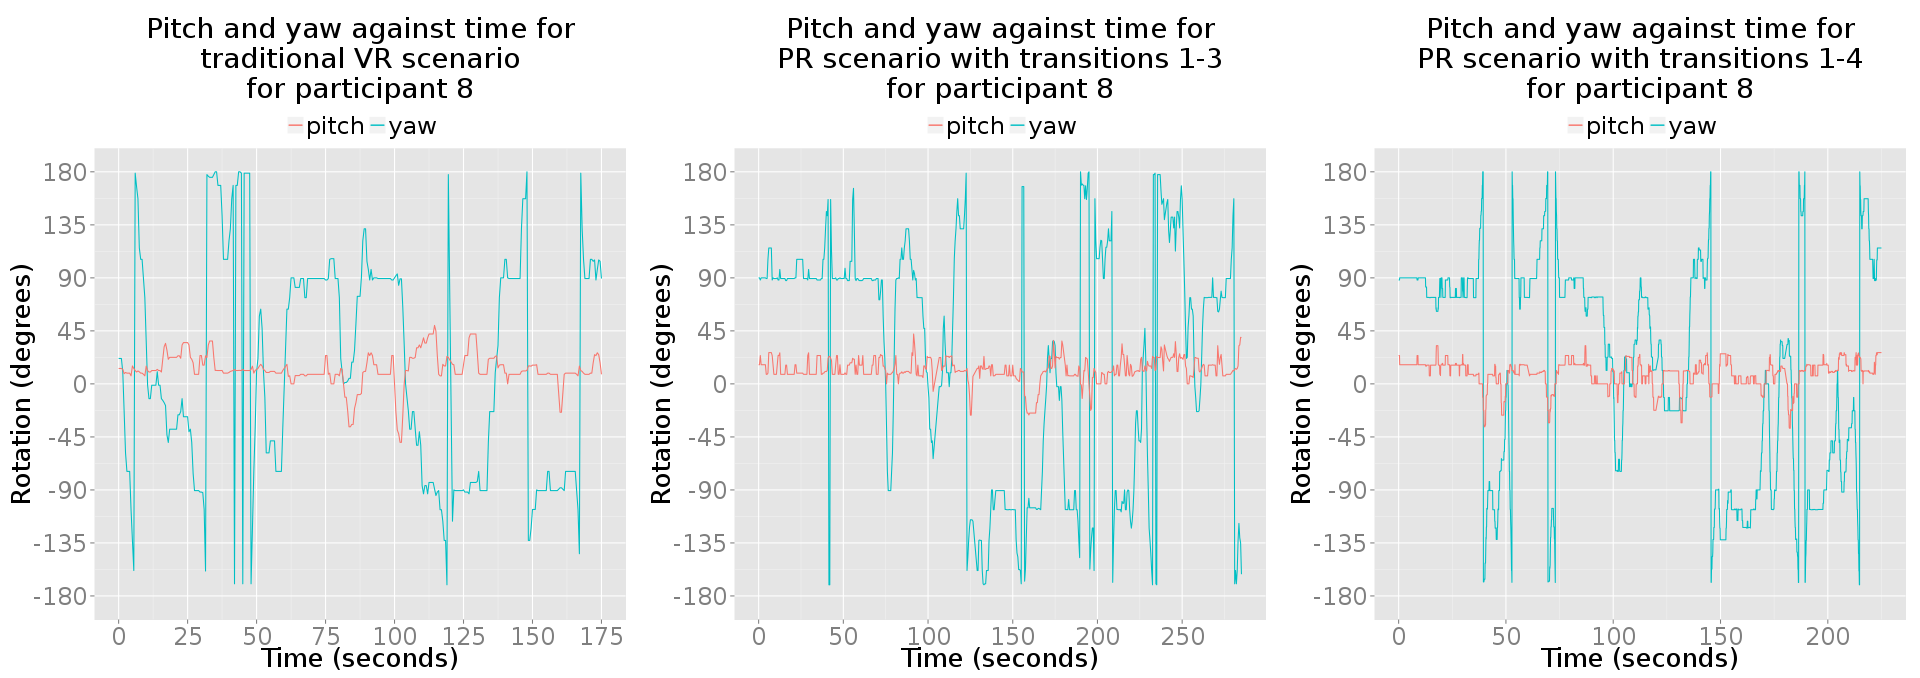
\includegraphics[width=\textwidth]{2.1/8-pitch-yaw-trad-1-3-1-4.png}
	\caption{Pitch and yaw against time for participant 8 in seated VR and both parallel reality scenarios.}
	\label{2-1-8-pitch-yaw-trad-1-3-1-4.png}
	\end{center}
\end{figure}

\begin{table}
\begin{center}
\begin{minipage}[t]{.45\linewidth}
\begin{center}
\begin{tabularx}{\textwidth}{c *{3}{>{\centering\arraybackslash}X}}
\toprule

\textbf{Participant} & \textbf{Pitch (\textdegree)} & \textbf{Yaw (\textdegree)} \\

\midrule

7 & 13.013 & 87.822 \\

8 & 13.917 & 94.436 \\

9 & 12.039 & 87.956 \\

10 & no data & no data \\

11 & no data & no data \\

12 & no data & no data \\

13 & no data & no data \\

\bottomrule
\end{tabularx}
\caption{Standard deviation in pitch and yaw for seated VR scenario.}
\label{2-1-sd-trad}
\end{center}
\end{minipage}
\end{center}
\end{table}

\begin{table}
\begin{center}
\begin{minipage}[t]{.45\linewidth}
\begin{center}
\begin{tabularx}{\textwidth}{c *{3}{>{\centering\arraybackslash}X}}
\toprule

\textbf{Participant} & \textbf{Pitch (\textdegree)} & \textbf{Yaw (\textdegree)} \\

\midrule

7 & no data & no data \\

8 & 10.253 & 102.254 \\

9 & 13.734 & 84.076 \\

10 & 17.833 & 84.578 \\

11 & 11.540 & 76.445 \\

12 & 19.635 & 74.696 \\

13 & 22.095 & 91.827 \\

\bottomrule
\end{tabularx}
\caption{Standard deviation in pitch and yaw for parallel reality scenario with transitions 1-3 (RW and VR periods combined).}
\label{2-1-sd-1-3}
\end{center}
\end{minipage}
%
\begin{minipage}[t]{.02\linewidth}
\hfill%
\end{minipage}
%
\begin{minipage}[t]{.45\linewidth}
\begin{center}
\begin{tabularx}{\textwidth}{c *{3}{>{\centering\arraybackslash}X}}
\toprule

\textbf{Participant} & \textbf{Pitch (\textdegree)} & \textbf{Yaw (\textdegree)} \\

\midrule

7 & no data & no data \\

8 & 11.493 & 89.531 \\

9 & 12.365 & 95.144 \\

10 & 14.059 & 90.429 \\

11 & 8.354 & 82.279 \\

12 & 22.202 & 75.425 \\

13 & 19.530 & 62.321 \\

\bottomrule
\end{tabularx}
\caption{Standard deviation in pitch and yaw for parallel reality scenario with transitions 1-4 (RW and VR periods combined).}
\label{2-1-sd-1-4}
\end{center}
\end{minipage}
\end{center}
\end{table}

%=====================

\newpage

Plots of position data upon the floorplan of the chapel highlight one situation in which the parallel reality scenarios served to restrict participant exploration compared to the seated VR scenario. During the seated VR scenario participants could move their virtual vantage through positions that were impossible to move through during the parallel reality scenarios due to the presence of real obstructions (an example of non-total spatial equivalence). Figures \ref{08-seatedmap.png} (seated VR scenario) and \ref{08-13map.png} (scenario 1-3) show this relationship using participant 8 as an example. In the seated VR scenario participant 8 walked around the nave (the open area on the left of the floorplan) however during the scenario 1-3 they were prevented from doing so due to the presence of rows of chairs set out throughout the real nave and thus were only able to walk down, parallel with one of the rows of chairs, toward the south facing door.

\TwoFig{splodge-maps/08-seatedmap.png}{Position data (red dots) during parallel reality scenario for participant 8.}{08-seatedmap.png}
       {splodge-maps/08-13map.png}{Position data (red dots) during scenario 1-3 for participant 8.}{08-13map.png}

%=====================

\subsubsection{Comparing RW and VR periods within parallel reality scenarios}

When comparing head pitch and yaw data between the RW and VR periods within the two parallel reality scenarios, five out of the seven participants displayed greater variance in yaw when perceiving VR stimuli than when perceiving RW stimuli for both scenario 1-3 and scenario 1-4. Figure \ref{8-1-3-pitch-yaw.png} illustrates an example of this relationship for participant 8 undertaking scenario 1-3 while figure \ref{12-1-4-pitch-yaw.png} illustrates the relationship for participant 12 undertaking scenario 1-4. Again the background colouring of the plots represents whether the participant was perceiving RW or VR visual stimuli at each particular time index, using different colours to indicate which transition style was used to transition to the VR stimuli: pink for transition 1, green for transition 2, yellow for transition 3 and dark blue for transition 4.

\begin{figure}
	\begin{center}
	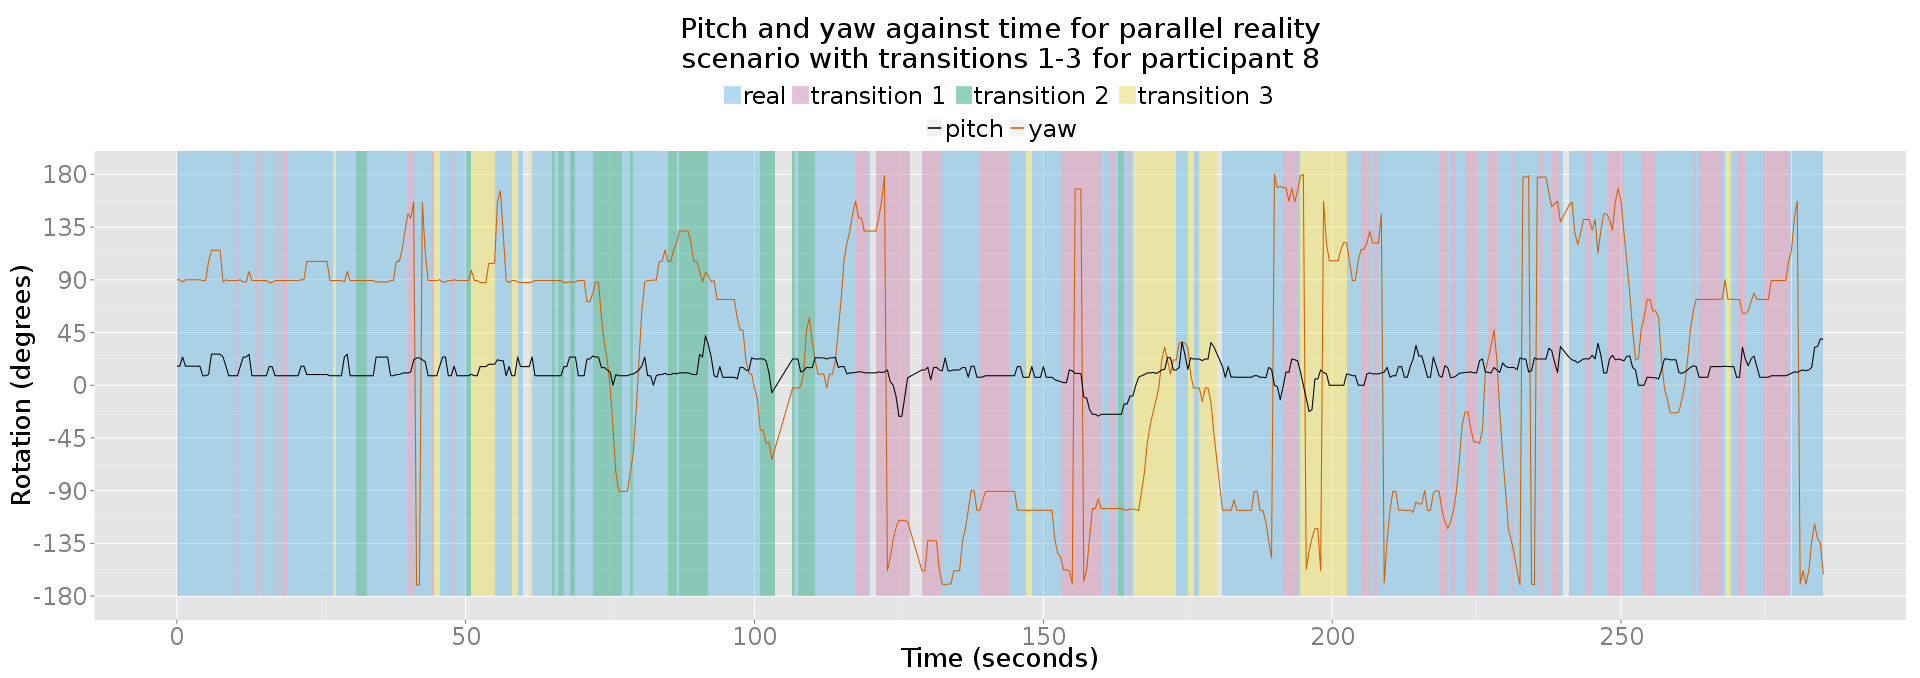
\includegraphics[width=\textwidth]{2.1/8-1-3-pitch-yaw.png}
	\caption{Pitch and yaw against time for participant 8 in scenario 1-3, showing RW/VR transitions.}
	\label{8-1-3-pitch-yaw.png}
	\end{center}
\end{figure}

%\begin{figure}
%	\begin{center}
%	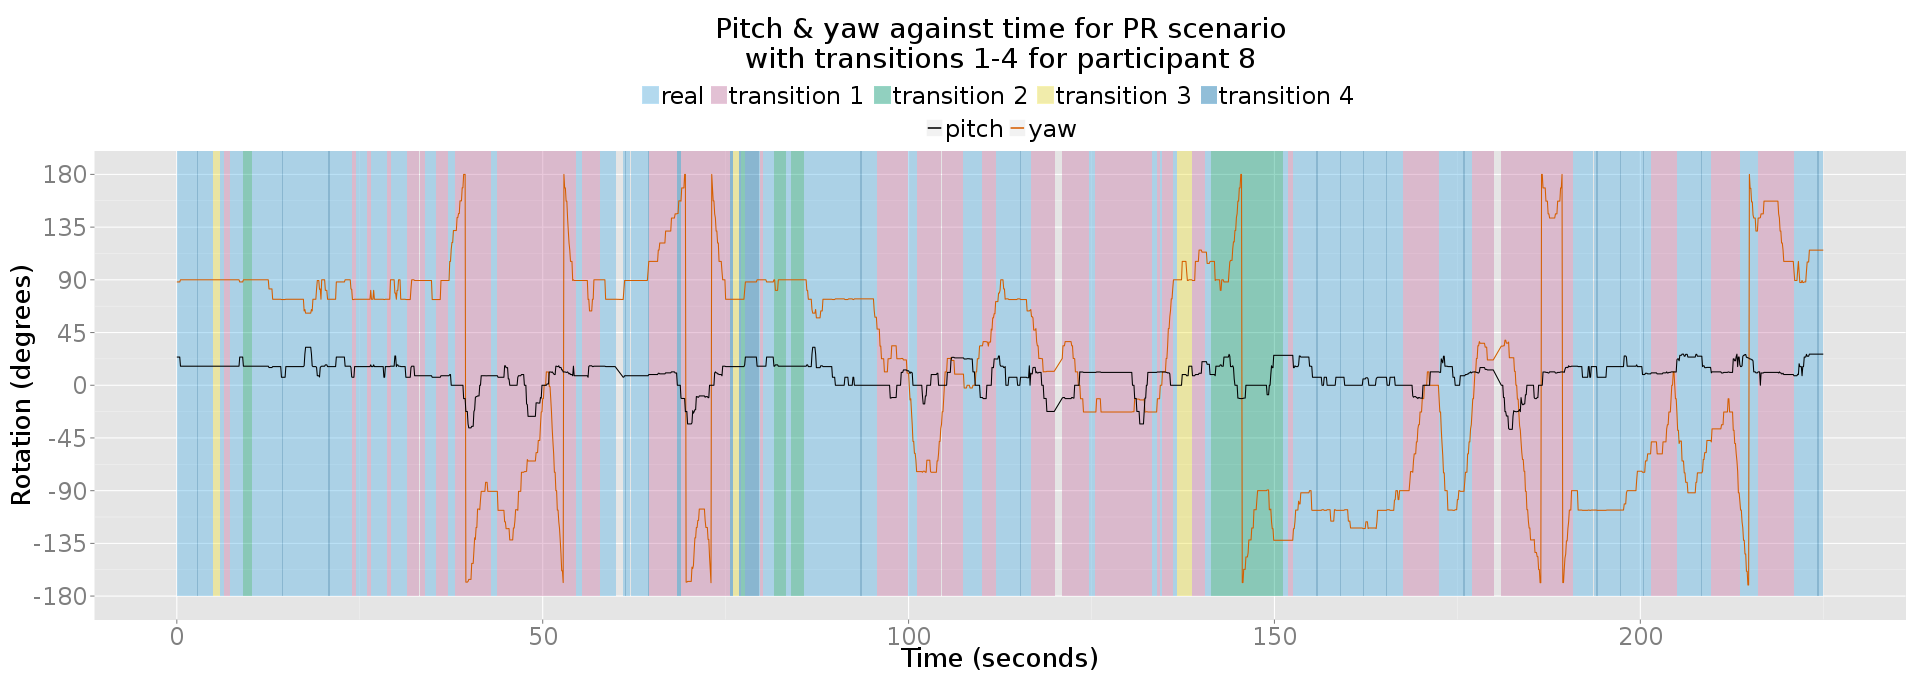
\includegraphics[width=\textwidth]{2.1/8-1-4-pitch-yaw.png}
%	\caption{Pitch and yaw against time for participant 8 in scenario 1-4, showing RW/VR transitions.}
%	\label{8-1-4-pitch-yaw.png}
%	\end{center}
%\end{figure}

\begin{figure}
	\begin{center}
	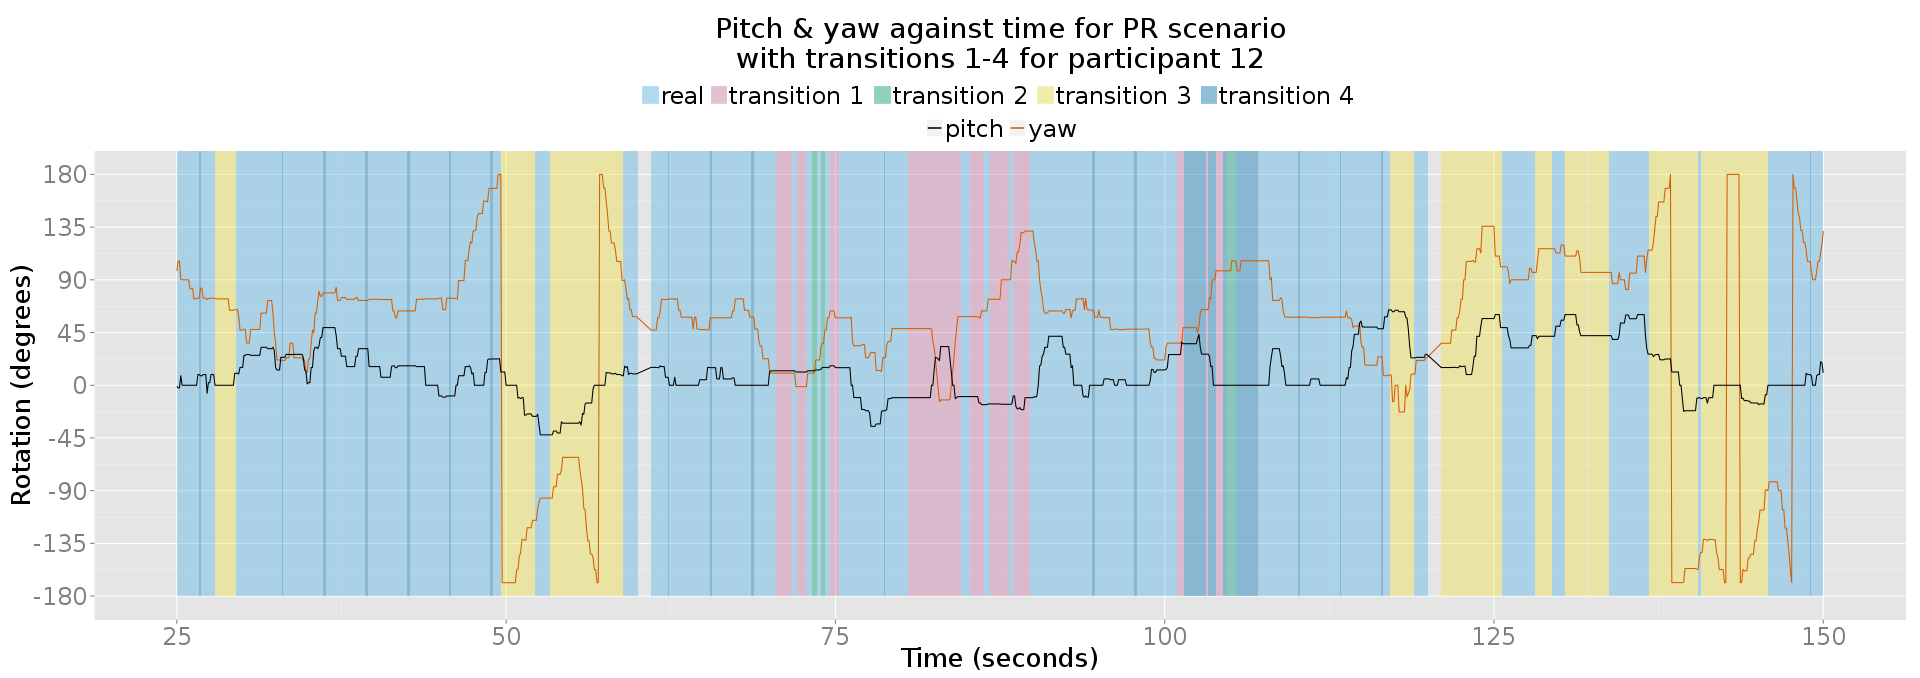
\includegraphics[width=\textwidth]{2.1/12-1-4-pitch-yaw.png}
	\caption{Pitch and yaw against time for participant 12 in scenario 1-4, showing RW/VR transitions.}
	\label{12-1-4-pitch-yaw.png}
	\end{center}
\end{figure}

\newpage

When comparing head movement as mean standard deviation weighted by duration of the periods (tables \ref{mean-sd-yaw-1-3} and \ref{mean-sd-yaw-1-4}) between the RW and VR portions of the two parallel reality scenarios, this relationship is seen much more substantially in scenario 1-4. Part of this is due to the fact that all participants in scenario 1-4 showed less change in yaw in the RW periods than in the RW periods of scenario 1-3. Whilst this apparent increased comfort with larger head movements in VR in scenario 1-4 could be explained due to familiarity, the magnitude of the difference between scenario 1-3 and scenario 1-4 makes it hard to believe that familiarity is the sole reason, especially considering that scenario 1-4 was not a drastically different experience to scenario 1-3 as only the addition of transition 4 differentiated it from scenario 1-3. One possible contributor, as mentioned by one participant during the interview stage, is that they spent more time perceiving VR in scenario 1-4 in order to \textit{avoid} the automatic transition that would occur when perceiving RW.

\vspace{1cm}

\begin{table}[h]
\begin{center}
\begin{minipage}[t]{.45\linewidth}
\begin{center}
\begin{tabularx}{\textwidth}{c *{3}{>{\centering\arraybackslash}X}}
\toprule

\textbf{Participant} & \textbf{RW (\textdegree)} & \textbf{VR (\textdegree)} \\

\midrule

7 & no data & no data \\

8 & 41.680 & 42.228 \\

9 & 19.274 & 31.133 \\

10 & 13.541 & 16.758 \\

11 & 28.030 & 16.751 \\

12 & 38.654 & 28.494 \\

13 & 29.623 & 39.717 \\

\bottomrule
\end{tabularx}
\caption{Weighted mean sd in yaw for scenario 1-3.}
\label{mean-sd-yaw-1-3}
\end{center}
\end{minipage}
%
\begin{minipage}[t]{.02\linewidth}
\hfill%
\end{minipage}
%
\begin{minipage}[t]{.45\linewidth}
\begin{center}
\begin{tabularx}{\textwidth}{c *{3}{>{\centering\arraybackslash}X}}
\toprule

\textbf{Participant} & \textbf{RW (\textdegree)} & \textbf{VR (\textdegree)} \\

\midrule

7 & 20.228 & 50.963 \\

8 & 10.783 & 50.593 \\

9 & 13.579 & 27.398 \\

10 & 10.7334 & 34.981 \\

11 & 13.500 & 13.513 \\

12 & 16.248 & 50.326 \\

13 & 7.269 & 57.162 \\

\bottomrule
\end{tabularx}
\caption{Weighted mean sd in yaw for scenario 1-4.}
\label{mean-sd-yaw-1-4}
\end{center}
\end{minipage}
\end{center}
\end{table}

%=====================

\subsubsection{Experimenting With Transition Styles}

Some participants showed behaviour where they `tried out' the different transition styles before adopting one that they then used predominantly throughout the rest of the scenario. Participant 11 showed this behaviour in its most extreme case during scenario 1-3, when s/he tried each transition style just once at the very beginning of the scenario and then only used transition 3 (via the right trigger \texttt{[RT]}) throughout the rest of the scenario (figure \ref{11-pitch-yaw-1-3.png}). However when s/he came to perform scenario 1-4, s/he seemed to take this opportunity as a second chance to experiment with all of the different transition styles, using transitions 1, 2 and 3 at different points throughout the scenario (figure \ref{11-pitch-yaw-1-4.png}).

\begin{figure}[h]
	\begin{center}
	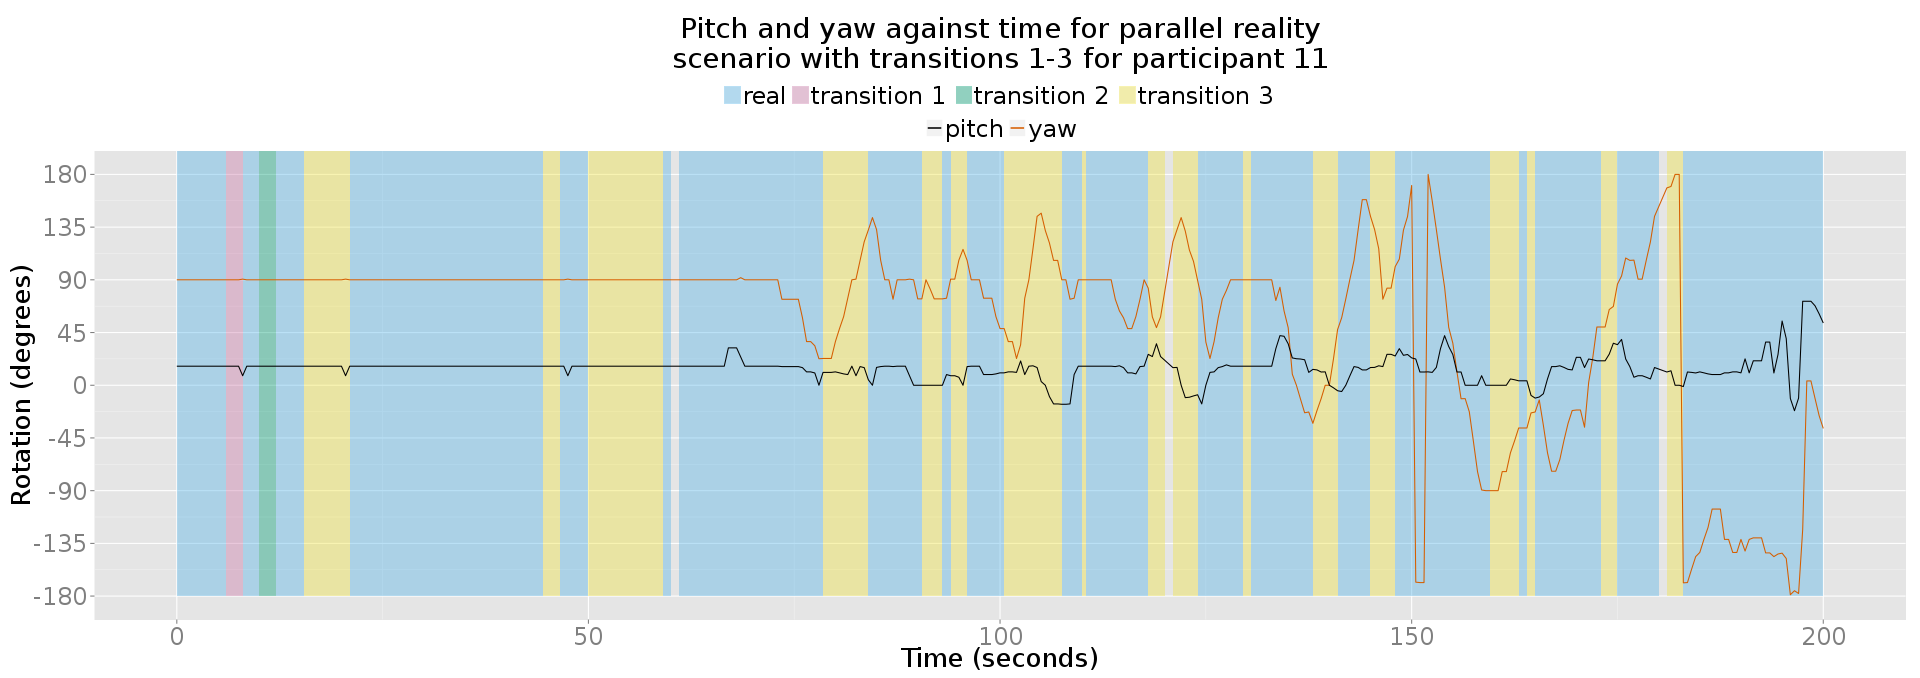
\includegraphics[width=\textwidth]{2.1/11-pitch-yaw-1-3.png}
	\caption{Pitch and yaw against time for participant 11 in scenario 1-3, showing RW/VR transitions.}
	\label{11-pitch-yaw-1-3.png}
	\end{center}
\end{figure}

\begin{figure}[h]
	\begin{center}
	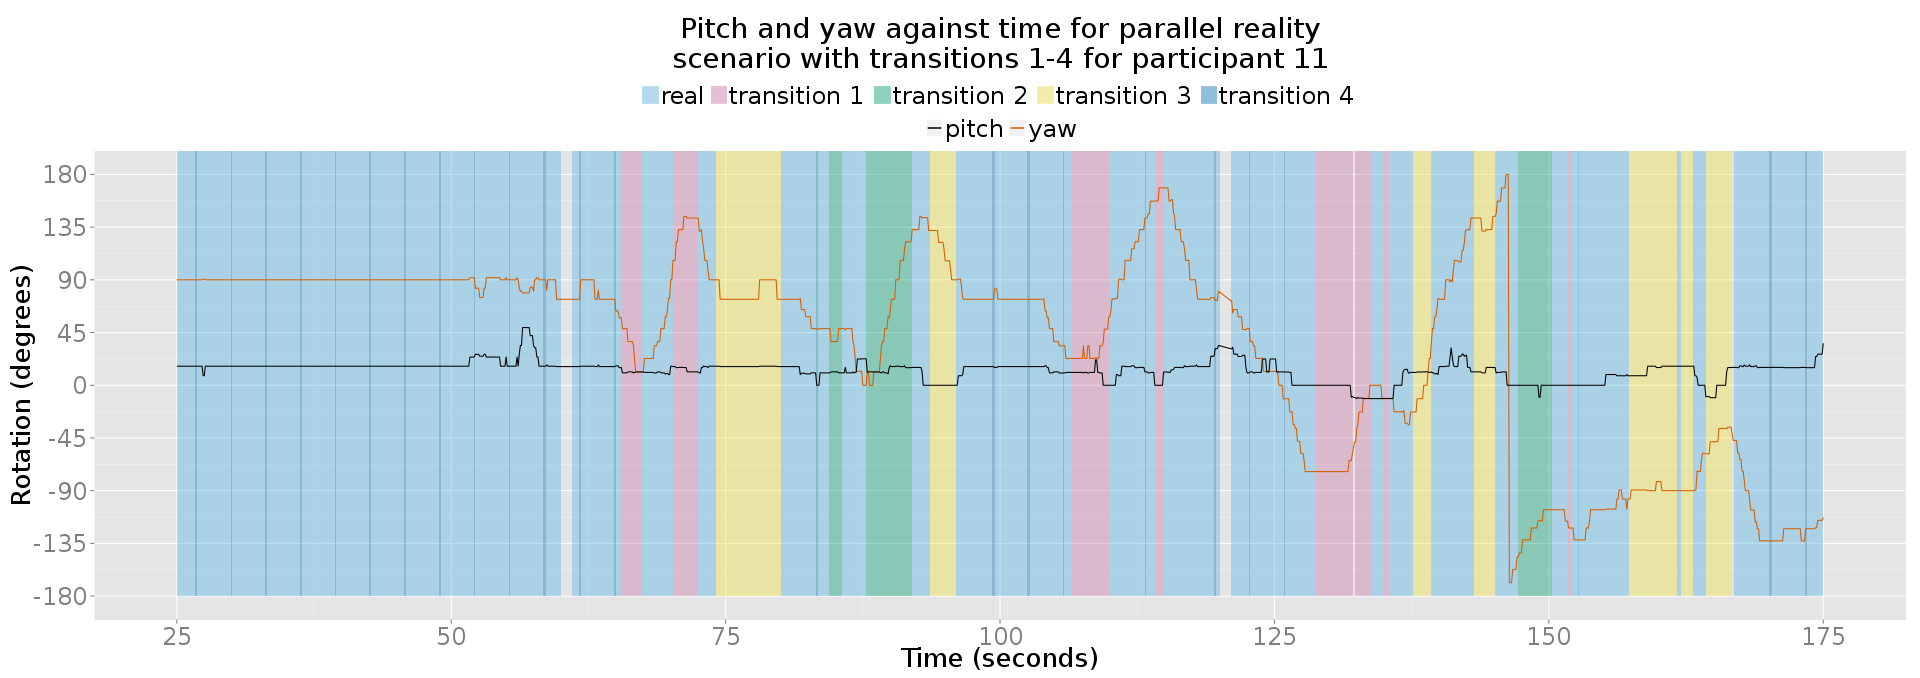
\includegraphics[width=\textwidth]{2.1/11-pitch-yaw-1-4.png}
	\caption{Pitch and yaw against time for participant 11 in scenario 1-3, showing RW/VR transitions.}
	\label{11-pitch-yaw-1-4.png}
	\end{center}
\end{figure}

%Participant 7 showed this behaviour in a less extreme fashion, spending more time with each of the three user-controllable transition styles before settling upon transition 3, during scenario 1-4 (figure \ref{7-pitch-yaw-1-4.png}).

%\begin{figure}
%	\begin{center}
%	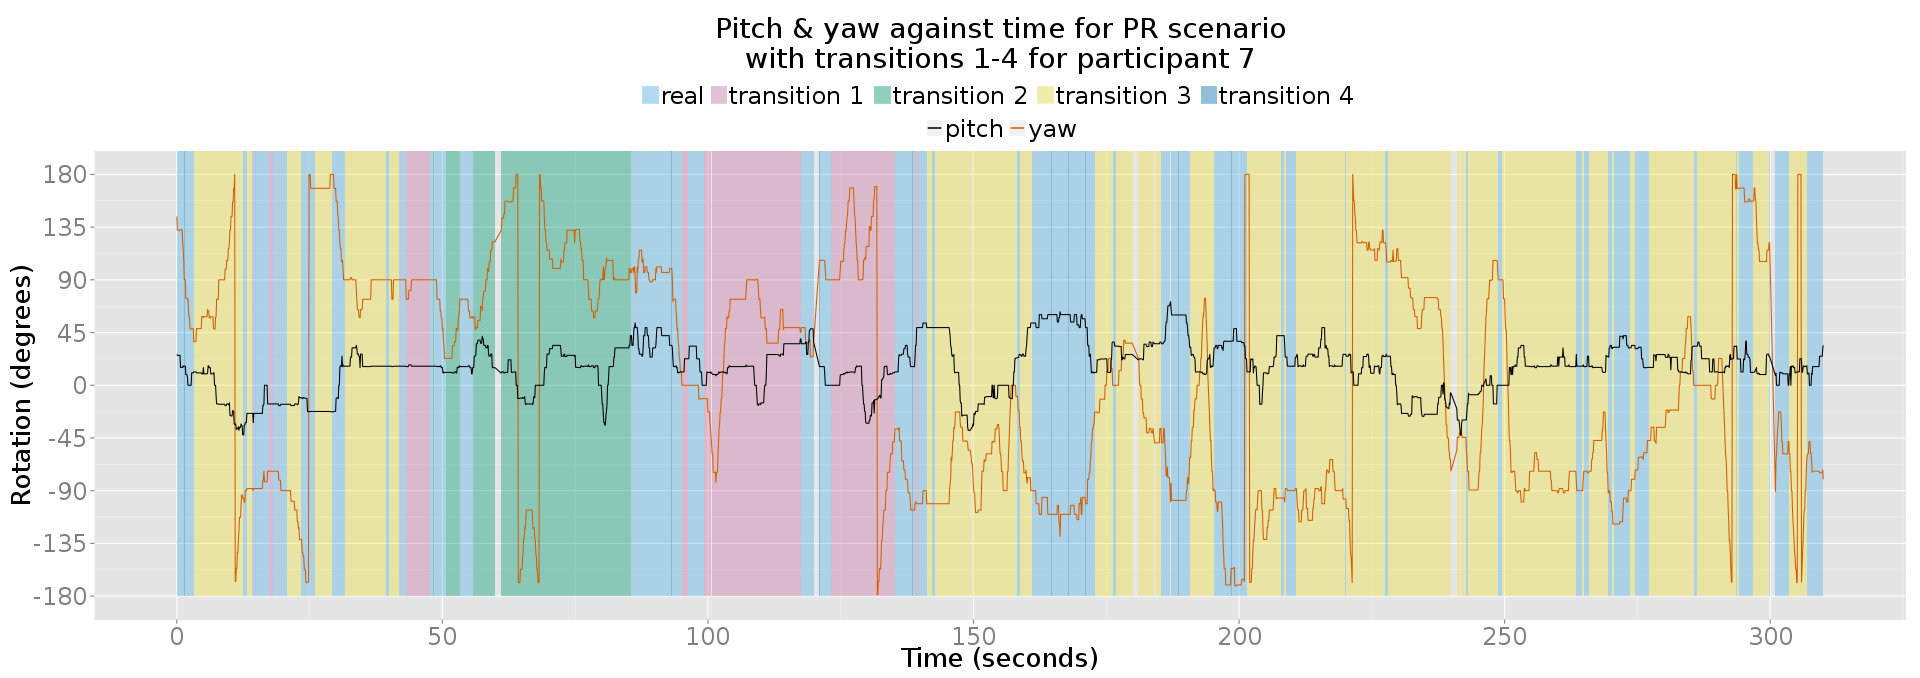
\includegraphics[width=\textwidth]{2.1/7-pitch-yaw-1-4.png}
%	\caption{Pitch and yaw against time for participant 7 in scenario 1-4, showing RW/VR transitions.}
%	\label{7-pitch-yaw-1-4.png}
%	\end{center}
%\end{figure}

\newpage

Other participants continued to use all available transition styles throughout a session, such as participant 13 during scenario 1-3 (figure \ref{13-pitch-yaw-1-3.png}). This was one of the longest individual sessions, with the participant exploring the RW and VR chapels in tandem in parallel reality via the Mirrorshades platform for over 8.5 minutes. During the interview s/he reported preferring transition 3 via the right trigger \texttt{[RT]}, which is corroborated by the data. S/he triggered this transition more than transition 1 or 2 (25 times total, compared to 20 for transition 1 and 14 for transition 2) and spent longer perceiving VR via transition 3 than the others (103 seconds total compared to 81.5 seconds for transition 1 and 20 seconds for transition 2, with a mean of 4.12 seconds for each period using transition 3, 4.075 seconds for transition 1 and 1.429 seconds for transition 2).

\begin{figure} [h]
	\begin{center}
	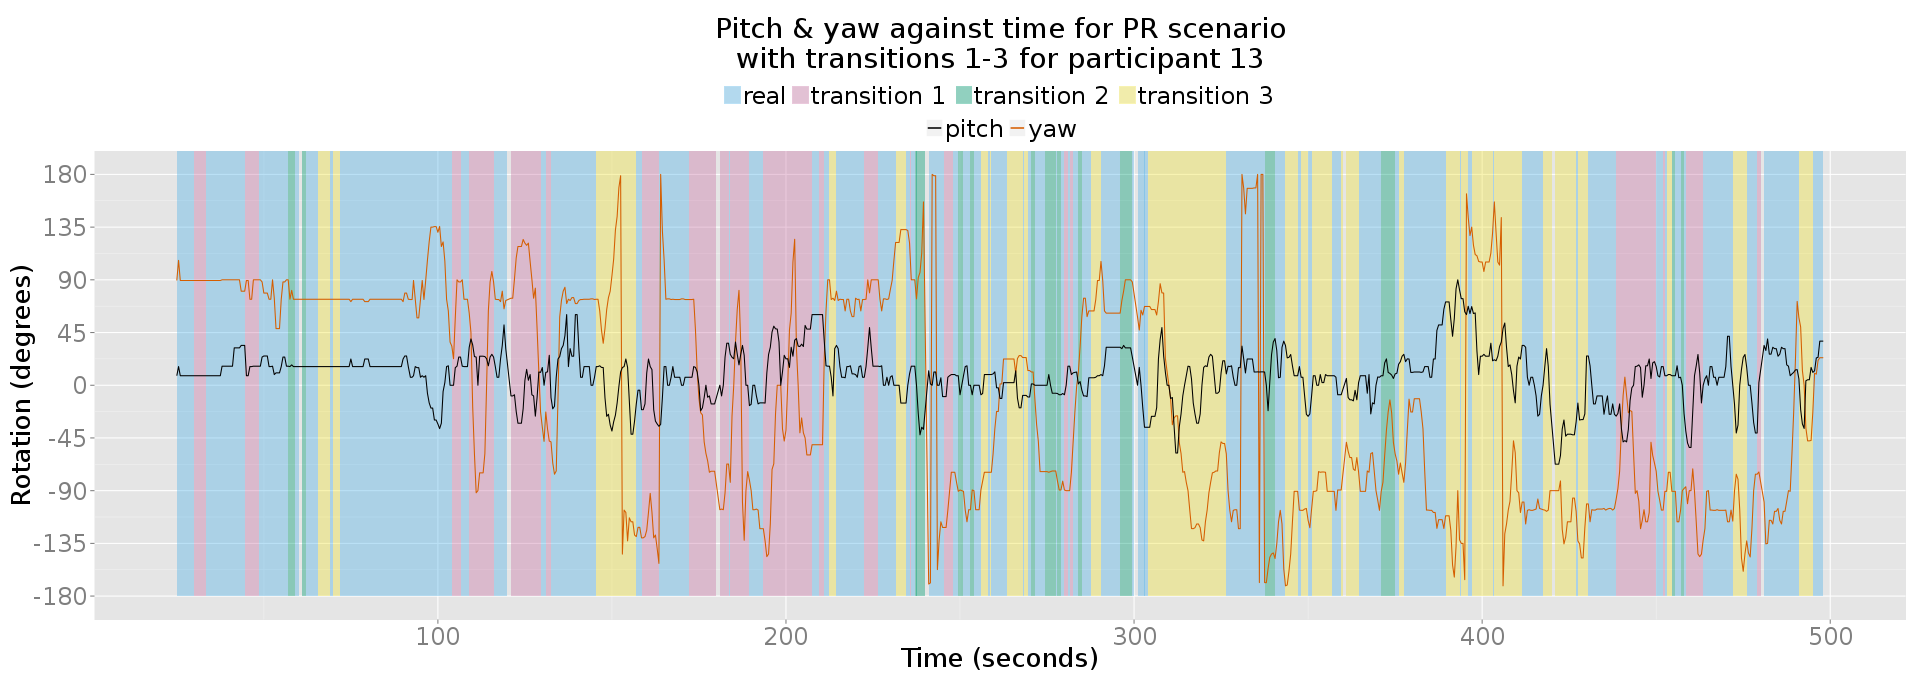
\includegraphics[width=\textwidth]{2.1/13-pitch-yaw-1-3.png}
	\caption{Pitch and yaw against time for participant 13 in scenario 1-3, showing RW/VR transitions.}
	\label{13-pitch-yaw-1-3.png}
	\end{center}
\end{figure}

%=====================

\newpage

\subsubsection{Walking and Head Movement}

As seen in the results to the stage 1 evaluation, there is also a correlation in the stage 2.1 results between position and change in head movement, with several participants displaying greater variance in head pitch and yaw while standing still than when walking with the DK1. This is true for both parallel reality scenarios; as an example figure \ref{8-1-3_2up.png} shows pitch and yaw against time above, aligned with distance moved against time below, for participant 8 performing scenario 1-3. Figure \ref{9-1-4_2up.png} shows the same arrangement for participant 9 performing scenario 1-4. Especially after taking into consideration the slight lag in IPS data, the stationary periods starting around 120, 160, 200 and 240 seconds in figure \ref{8-1-3_2up.png} and those starting around 70, 150 and 210 seconds in figure \ref{9-1-4_2up.png}, all closely coincide with pronounced variance in yaw.

\begin{figure}
	\begin{center}
	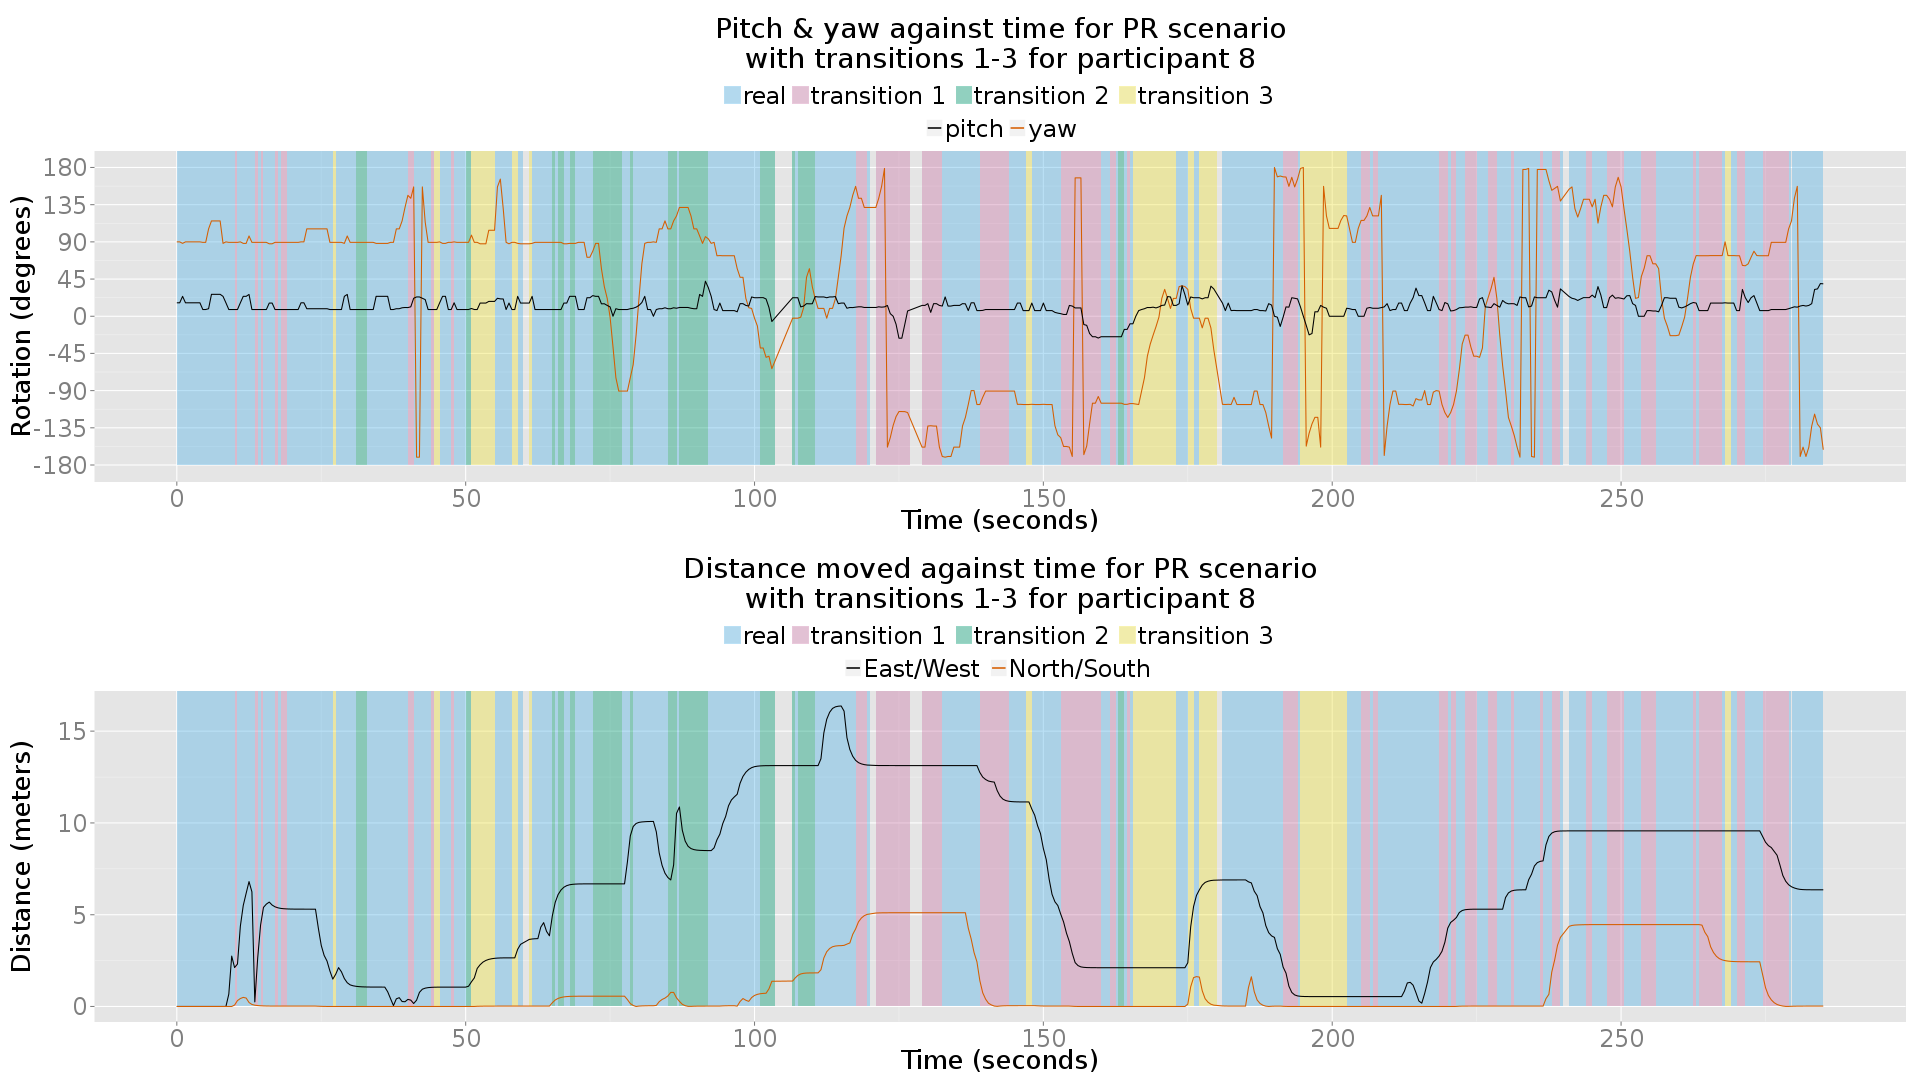
\includegraphics[width=\textwidth]{2.1/8-1-3_2up.png}
	\caption{Pitch and yaw against time aligned with distance moved against time for participant 8 in scenario 1-3, showing RW/VR transitions.}
	\label{8-1-3_2up.png}
	\end{center}
\end{figure}

\begin{figure}
	\begin{center}
	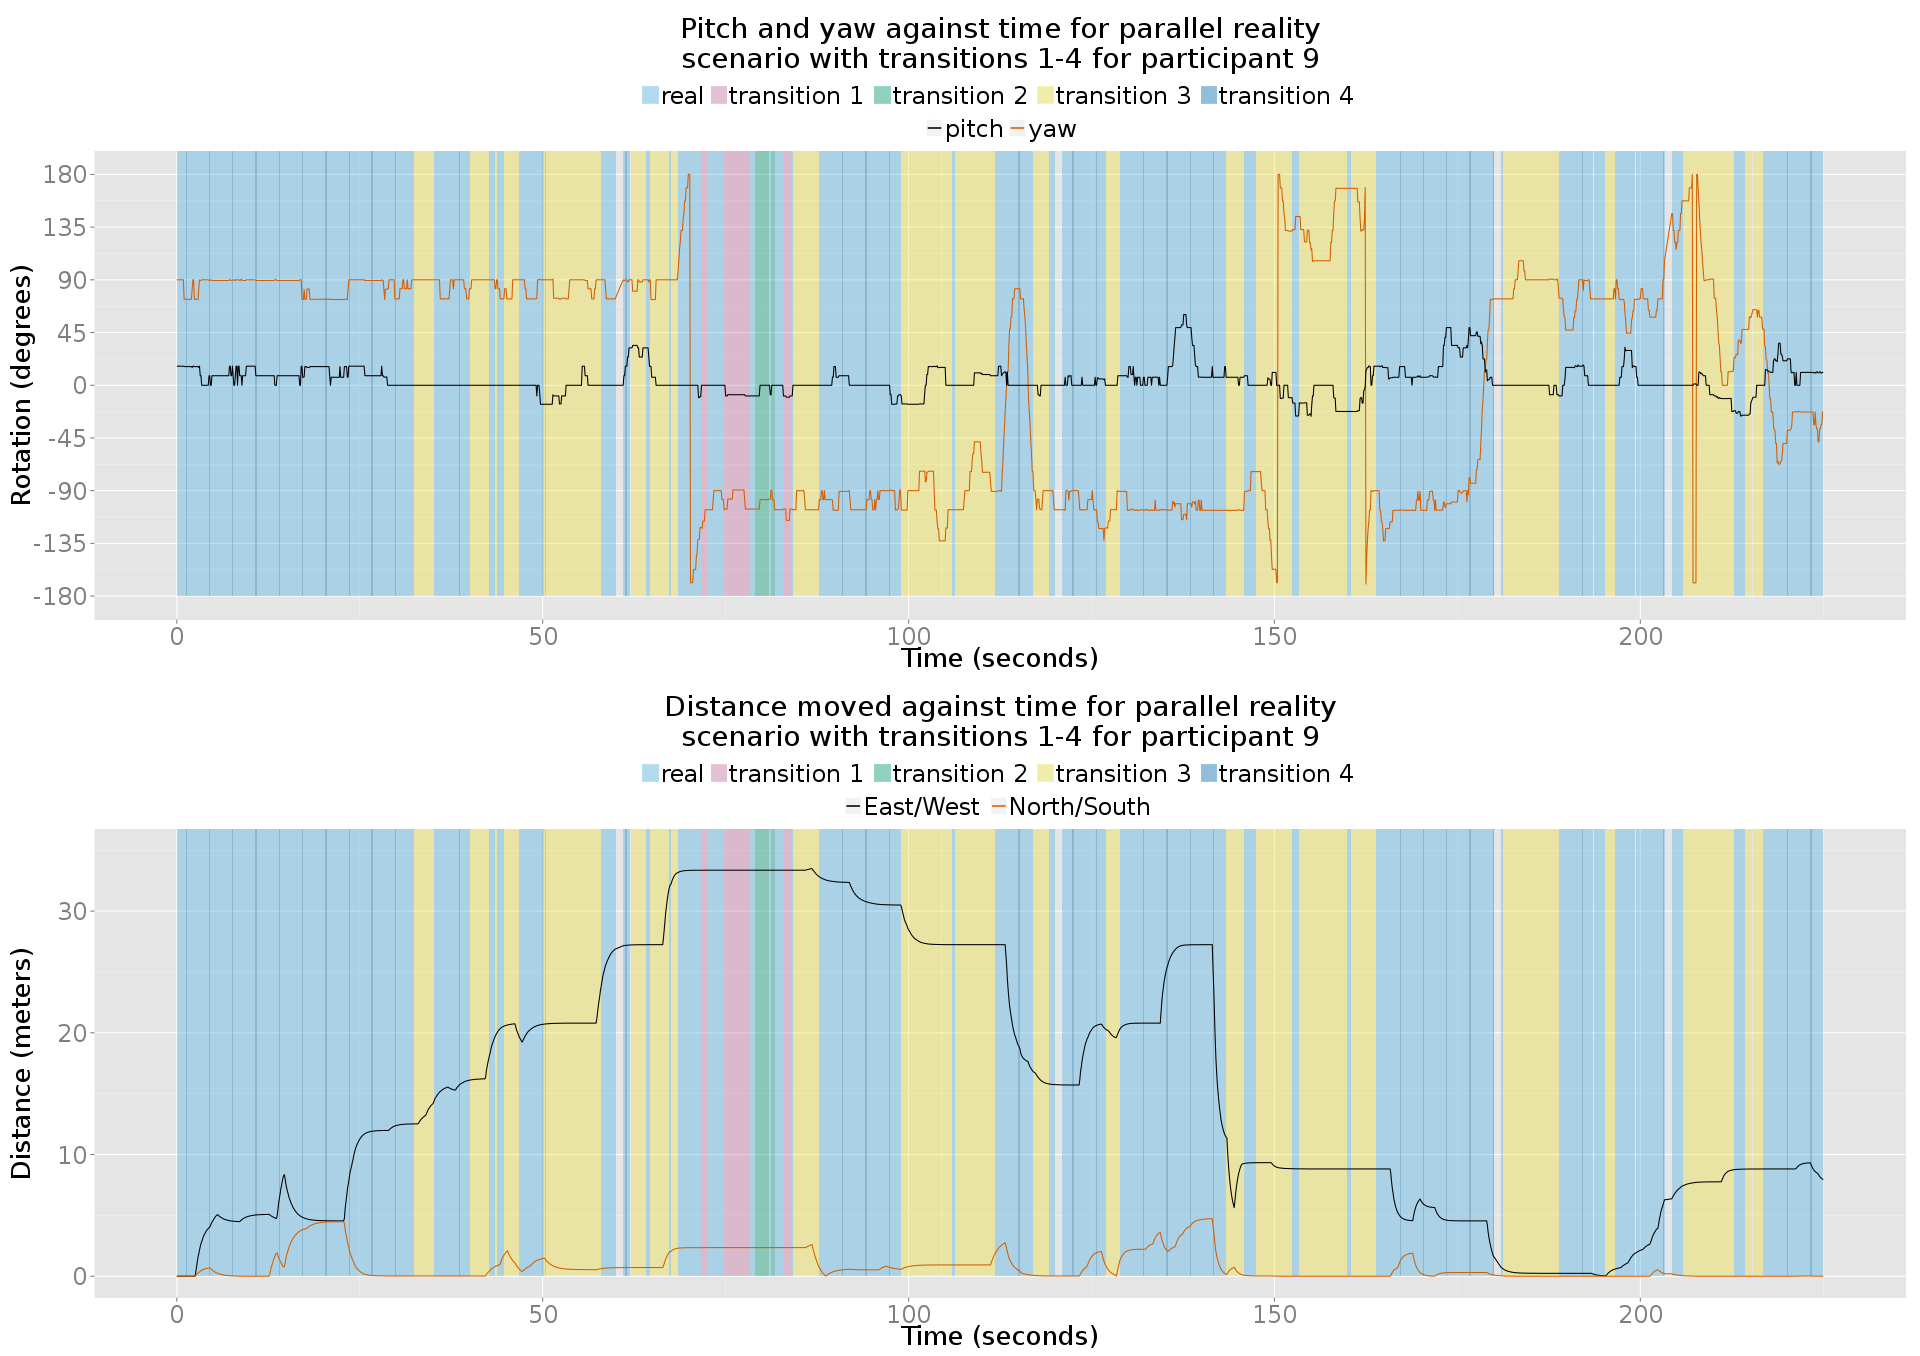
\includegraphics[width=\textwidth]{2.1/9-1-4_2up.png}
	\caption{Pitch and yaw against time aligned with distance moved against time for participant 9 in scenario 1-4, showing RW/VR transitions.}
	\label{9-1-4_2up.png}
	\end{center}
\end{figure}

%=====================

\newpage

\subsubsection{Use of Intermediary Opacities}

Confirming responses during the post task interviews, several participants made use of the analogue selectable transition (transition 3, accessed via the right trigger \texttt{[RT]}) to view both RW and VR environments together, by pausing with the trigger partially depressed. Figures \ref{10-1-4_opacity.png} and \ref{12-1-4_opacity.png} show examples, for participants 10 and 12 respectively undertaking scenario 1-4, of the opacity of the objects upon which the camera feeds were rendered. An opacity of 1.0 means that the camera feeds were completely opaque and that the participant was thus perceiving 100\% RW visual stimuli, while an opacity of 0 means that the camera feeds were invisible and that the participant was perceiving 100\% VR visual stimuli. As well as using the analogue selectable transition to view both environments at once, there are incidents where it seems that the participant used it to control the speed at which a transition from 100\% RW to 100\% VR was performed. We can see that participant 10 (figure \ref{10-1-4_opacity.png}) uses transition 3 at around 250 seconds to perform a transition to a 100\% VR view, but at a slower rate than the linear interpolated transition such as can be seen taking place just before at around 245 seconds. This greater level of control in how quickly transitions were performed was raised in interviews as one reason why this particular transition was favoured by participants.

\vspace{2cm}

\begin{figure}[h]
	\begin{center}
	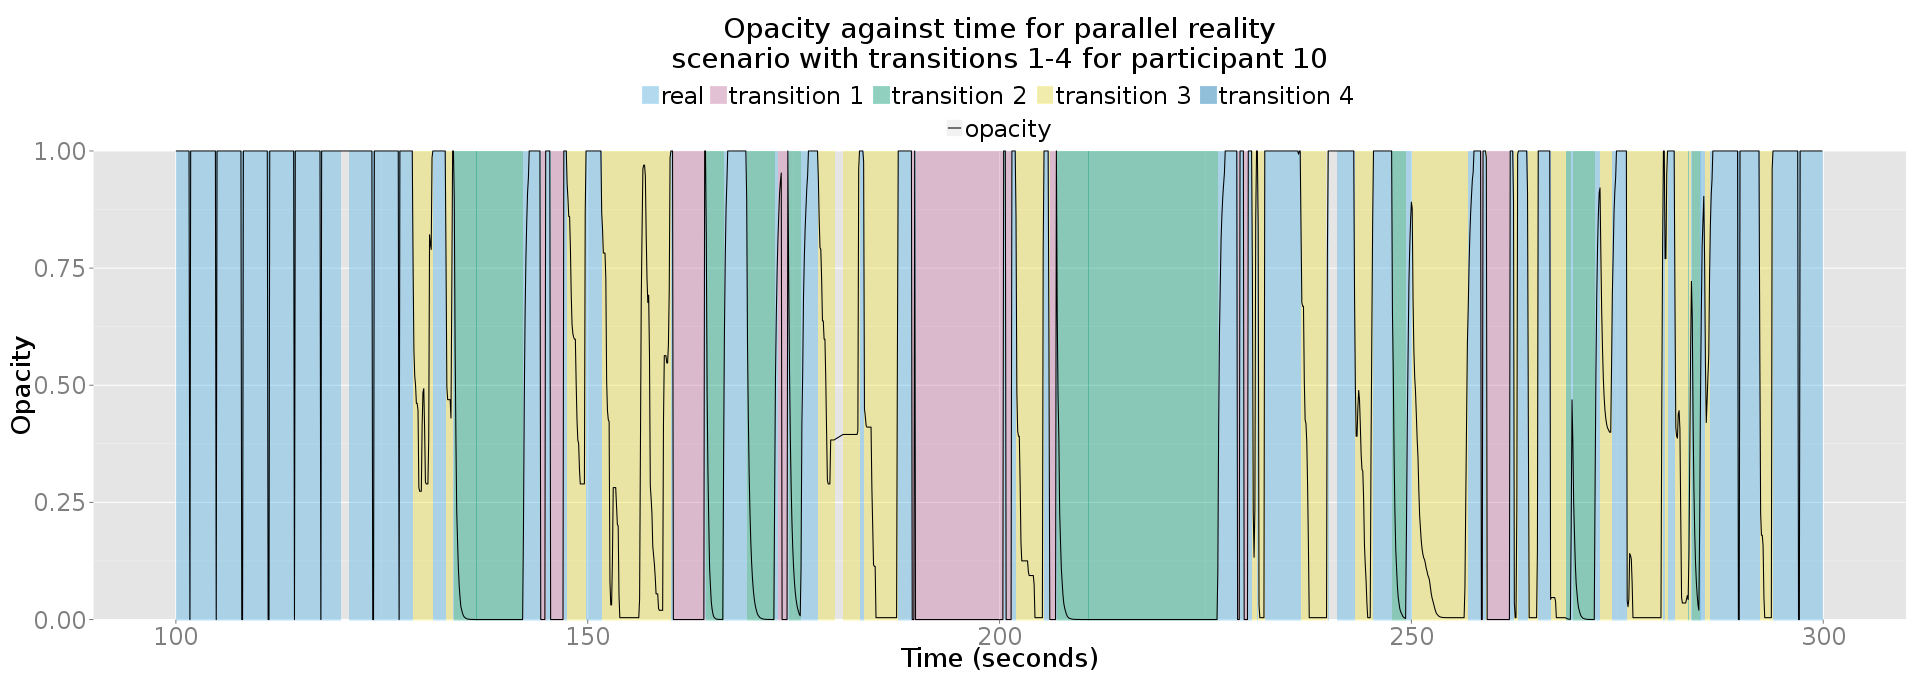
\includegraphics[width=\textwidth]{2.1/10-1-4_opacity.png}
	\caption{Opacity of camera objects against time for participant 10 in scenario 1-4, showing RW/VR transitions.}
	\label{10-1-4_opacity.png}
	\end{center}
\end{figure}

\begin{figure}
	\begin{center}
	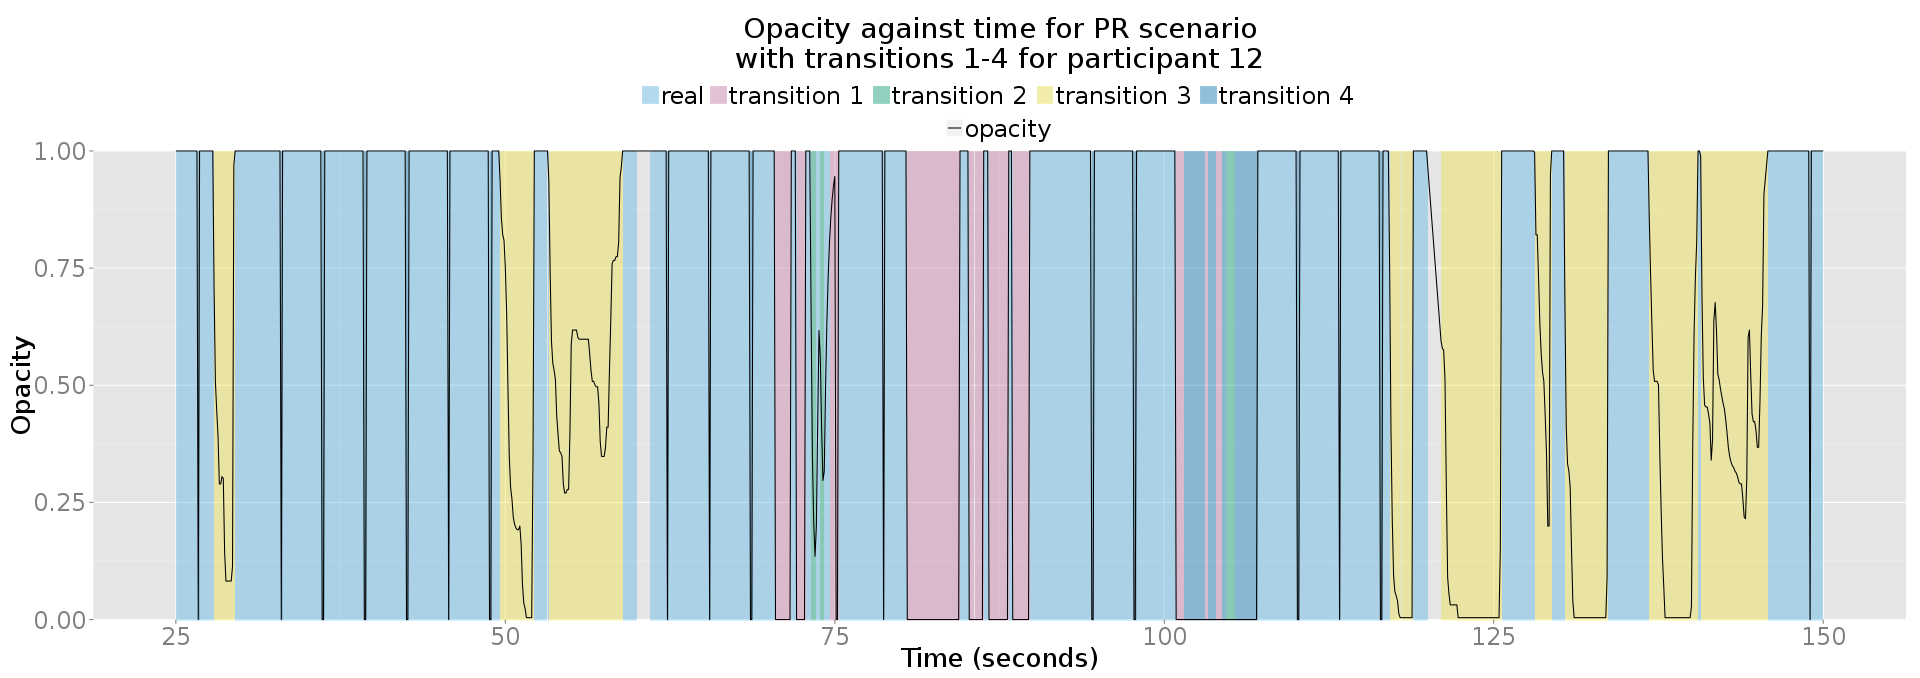
\includegraphics[width=\textwidth]{2.1/12-1-4_opacity.png}
	\caption{Opacity of camera objects against time for participant 12 in scenario 1-4, showing RW/VR transitions.}
	\label{12-1-4_opacity.png}
	\end{center}
\end{figure}

%=====================
	
%Other
%	participant 12 - all big head movements in 1-4 were in VR, but in 1-3 there was RW head movement too?


%Number of transitions in each session ranged from high teens to low sixties.

%Mean times spent in real/virtual are much closer than in stage 1.
%Time spent in virtual
%	participant 8 - more time spent in VR in 1-4 to avoid the automatic switch
%	participant 9 - more time spent in VR because of better understanding what they were meant to be doing (familiarity)


%four of seven participants spent more time in real than virtual in both 1-3 and 1-4
%	for three participants the ratio was closer in 1-4 than in 1-3 (avoiding transition 4?)
%	one spent more time in virtual than real in both 1-3 and 1-4
%	one spent more time in real in 1-3 and then more time in virtual tin 1-4 (familiarity?)

%=========================================================================================================

\newpage

\subsection{IPQ}

IPQ results were scaled from the -3 to +3 range used by the questionnaires to the 0 to 6 range used to express results herein. The reversed items (SP2, INV3 and REAL1) had their results appropriately reversed. Tables \ref{sp-2-1-table}, \ref{inv-2-1-table} and \ref{real-2-1-table} show the mean and standard deviation for SP, INV and REAL respectively for the all of the scenarios (seated VR scenario, scenario 1-3 and scenario 1-4).

\begin{table}[h]
\begin{center}
\begin{minipage}[t]{.45\linewidth}
\begin{center}
\begin{tabularx}{\textwidth}{c *{3}{>{\centering\arraybackslash}X}}
\toprule

\textbf{Scenario} & \textbf{Mean} & \textbf{Standard deviation} \\

\midrule

seated & 4.6 & 0.780 \\

1-3 & 4.133 & 1.093 \\

1-4 & 4.133 & 0.532 \\

\bottomrule
\end{tabularx}
\caption{Means and standard deviations of SP for all stage 2.1 scenarios.}
\label{sp-2-1-table}
\end{center}
\end{minipage}
%
\begin{minipage}[t]{.02\linewidth}
\hfill%
\end{minipage}
%
\begin{minipage}[t]{.45\linewidth}
\begin{center}
\begin{tabularx}{\textwidth}{c *{3}{>{\centering\arraybackslash}X}}
\toprule

\textbf{Scenario} & \textbf{Mean} & \textbf{Standard deviation} \\

\midrule

seated & 4.166 & 1.393 \\

1-3 & 2.666 & 1.125 \\

1-4 & 1.958 & 1.308 \\

\bottomrule
\end{tabularx}
\caption{Means and standard deviations of INV for all stage 2.1 scenarios.}
\label{inv-2-1-table}
\end{center}
\end{minipage}

\vspace{5mm}

\begin{minipage}[t]{.45\linewidth}
\begin{center}
\begin{tabularx}{\textwidth}{c *{3}{>{\centering\arraybackslash}X}}
\toprule

\textbf{Scenario} & \textbf{Mean} & \textbf{Standard deviation} \\

\midrule

seated & 2.208 & 1.134 \\

1-3 & 1.917 & 1.339 \\

1-4 & 1.917 & 1.080 \\

\bottomrule
\end{tabularx}
\caption{Means and standard deviations of REAL for all stage 2.1 scenarios.}
\label{real-2-1-table}
\end{center}
\end{minipage}
%
\begin{minipage}[t]{.02\linewidth}
\hfill%
\end{minipage}
%
\begin{minipage}[t]{.45\linewidth}
\begin{center}
\begin{tabularx}{\textwidth}{c *{5}{>{\centering\arraybackslash}X}}
\toprule

\textbf{Scenario} & \multicolumn{2}{c}{\textbf{SP3}} & \multicolumn{2}{c}{\textbf{INV2}} \\

\cmidrule(l){2-3} \cmidrule(l){4-5}

 & \textbf{mean} & \textbf{sd} & \textbf{mean} & \textbf{sd} \\
 
\midrule

seated & 4.5 & 1.472 & 4 & 1.673 \\

1-3 & 2.5 & 2.160 & 2.8 & 1.643 \\

1-4 & 3.5 & 1.633 & 1 & 0.707 \\
 
\bottomrule
\end{tabularx}
\caption{Means for SP3 and INV2 for all stage 2.1 scenarios.}
\label{sp3-inv2-2-1-table}
\end{center}
\end{minipage}
\end{center}
\end{table}

The seated VR scenario produced baseline IPQ results for a seated, full immersion HMD based VR experience in which RW stimuli are intentionally suppressed from the user. SP and INV results for this scenario were relatively high, while the REAL results were low. This does not come as much of a surprise, as the graphical quality of the VR chapel reconstruction used throughout the user studies was not stellar, partly as a result of having to intentionally reduce the level of detail in order to maintain acceptable framerates throughout the evaluations. It should come as no surprise then that even though participants perceived bodily actions to be possible within the VR environment (high SP) and found incompatible RW stimuli well suppressed (high INV) that the realness of the VR environment was nonetheless lacking (low REAL). As one participant said during their interview, it felt real even though it didn't look it: \textit{``\ldots obviously it wasn't the same quality, but I still felt so immersed in it. Even though part of me would've known it wasn't real, most of it felt real even though it didn't look like it''}.

In both parallel reality scenarios SP and REAL were reduced equally by a small amount, whilst INV was reduced more substantially and with a greater reduction for scenario 1-4 than for scenario 1-3. This met the hypothesis that a positively received parallel reality experience would result in noticeably reduced INV but without substantial reduction in SP and REAL. The reduced INV indicates that participants were more aware of RW stimuli, but the only marginally reduced SP indicates that their sense of presence in the VR environment did not drastically suffer because of this, indicating some mitigation of the effects of the extended vacancy problem. Furthermore the marginal reduction in REAL indicates that the perceived realness of the VR environment did not substantially suffer from tandem observation with the equivalent vantage point into the (necessarily real) RW environment. However the parallel reality experience was evidently not received positively enough to elicit heightened overall SP results as was hypothesized might happen.

Looking specifically at the results for SP3 and INV2 (table \ref{sp3-inv2-2-1-table}) they seem to be tied together as per Constantin's observation (see section \ref{igroup-presence-questionnaire-explanation}) for the seated VR scenario and scenario 1-3 where they fall equally. However in scenario 1-4, INV2 drops substantially more than SP3 which climbs to above its level in scenario 1-3. This lends support to the notion that in a parallel reality experience in which the user is encouraged (or \textit{forced} as was the case in scenario 1-4 with the automatic transitions) to view visual stimuli from two compatible environments that SP can be maintained, that the break in presence associated with a transition from one environment to the other is not so great as to effect a Gestalt switch and throw off perceptual/concrete processing to an extent that sense of presence (in terms of focus of attention) is drastically reduced.

%=========================================================================================================

\subsection{Graphical Performance}
\label{stage-2-1-framerates}
Framerates throughout the stage 2.1 evaluation (see figure \ref{framerates_2-1.png}) were largely as was to be expected after the platform's performance in stage 1 (see section \ref{stage-1-framerates}) with the seated VR scenario achieving slightly higher overall framerates with a mean of 53.2 fps (for the 3 participants for which these data were recorded) than the parallel reality scenarios that averaged 44.5 fps in scenario 1-3 and 41.1 fps in scenario 1-4. The difference between the seated VR scenario and the parallel reality scenarios was smaller than in the stage 1 evaluation, with the parallel reality scenarios exhibiting a 16.4\% slowdown compared to the 25.2\% slowdown seen in stage 1. The explanation for this is not immediately clear; it could be related to the introduction of the ability to view both real and virtual environments simultaneously via transition 3, which may be less complex to render in terms of the culling masks than completely culling real or virtual visuals, or it could simply be a result of a newer graphics driver leading to improved performance.

\begin{figure}[h]
	\begin{center}
	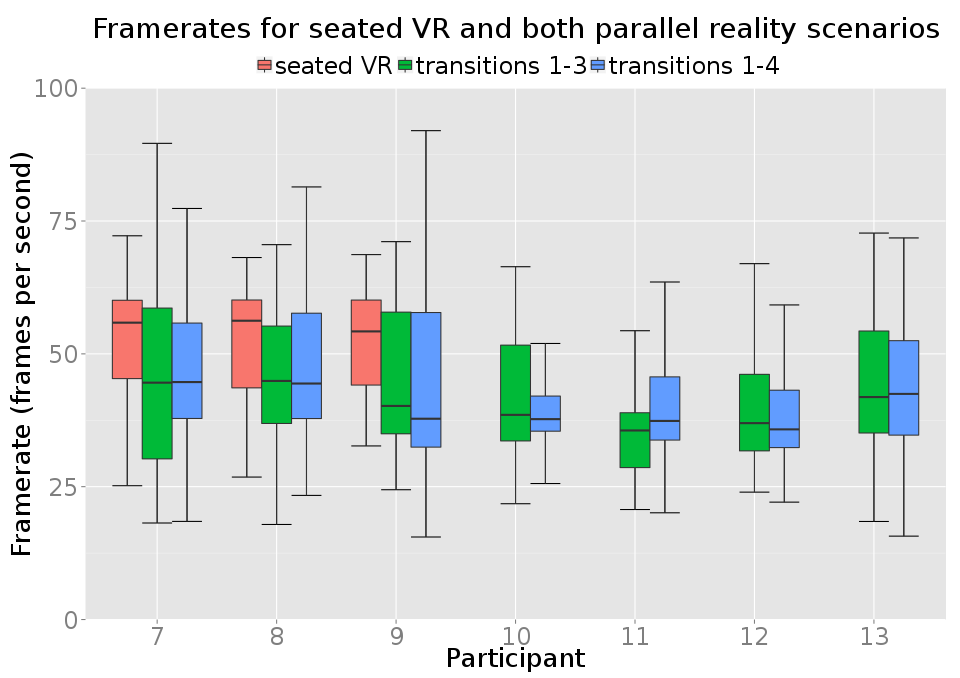
\includegraphics[width=.6\textwidth]{2.1/framerates_2-1.png}
	\caption{Framerates for seated VR and both parallel reality scenarios for all participants.}
	\label{framerates_2-1.png}
	\end{center}
\end{figure}

%=========================================================================================================

\subsection{IndoorAtlas Performance}

Performance of IndoorAtlas throughout both scenario 1-3 (figure \ref{2-1-positiondeltas1-3.png}) and scenario 1-4 (figure \ref{2-1-positiondeltas1-4.png}) was once again good, with the vast majority of movements being of a small scale and with the medians for all participants approaching 0 metres indicating that IndoorAtlas reliably identified stationary participants. Large jarring virtual movements were uncommon, however participants noted that when such a movement or inaccuracy coincided with an automatic transition the effect was unpleasant.

\TwoFig{2.1/2-1-positiondeltas1-3.png}{Distance between subsequent IndoorAtlas position data for scenario with transitions 1-3.}{2-1-positiondeltas1-3.png}
       {2.1/2-1-positiondeltas1-4.png}{Distance between subsequent IndoorAtlas position data for scenario with transitions 1-4.}{2-1-positiondeltas1-4.png}

Plots of position data upon the floorplan of the chapel illustrate how these occasional larger displacements could be particularly unpleasant when they coincided with the participant observing the virtual environment, due to the manner in which the virtual vantage would always follow the shortest/most direct path between subsequent positions, causing it to `pass through' any virtual obstructions along this path. Figures \ref{10-13map.png} and \ref{10-14map.png} show position data for participant 10 during scenario 1-3 and scenario 1-4 respectively. In scenario 1-3 the position data mostly fall on or close to the mapped IndoorAtlas routes (see figure \ref{sallies-indoor-atlas-routes.png}), however during scenario 1-4 there are position data outwith these routes and `in the middle' of virtual obstructions. For example, at one point a position was reported within the pews at the North wall of the building. A subsequent position was reported at the door adjacent to the tomb at the East end of the North wall of the building. Whilst both of these positions were occupiable by the participant in both the real and virtual environments, the direct path between them that the virtual vantage navigated (and upon which there are several reported positions due to the duration of this virtual movement) was not possible: it required the virtual vantage to pass through the actual seats/backs of the pews and partly through the North wall itself, an unpleasant experience when wearing a HMD.

\TwoFig{splodge-maps/10-13map.png}{Position data (red dots) during scenario 1-3 for participant 8.}{10-13map.png}
       {splodge-maps/10-14map.png}{Position data (red dots) during scenario 1-4 for participant 8.}{10-14map.png}

Where inaccuracies such as these are unavoidable in a parallel reality system, the negative effects that the resulting large movements pose should be minimised. Prudent approaches would be to specify a certain threshold for discrete movements, above which the user is either prevented from viewing virtual stimuli or for which the stimuli are blurred, dimmed or similarly obscured (along with a message/dialogue explaining the situation). Similar checks to prevent or mitigate the effect of the virtual vantage moving through virtual obstructions, even where the total movement is beneath the threshold value, would also be prudent.

%=========================================================================================================

\subsection{Stage 2.1 Summary}

This stage of the evaluation provided a first insight into best practices for implementing future parallel reality experiences, by evaluating preferences and reactions toward different implementations of the first of the two fundamental aspects of performing transitions between RW and VR visual stimuli discussed in section \ref{design-considerations-for-rw-vr-transitions}; the process by which the visual stimuli of one environment are replaced by those of the other environment. The ability to manually control the balance of RW/VR visuals emerged as preferable to more basic transitions that simply alternated between the default view and the VR view at set speeds, while adding uncontrolable moments of VR visuals to the default view led to a negative effect upon enjoyment and comfort but a positive effect upon observation and understanding of the relationship between the two constituent environments.

Participants overwhelmingly preferred transition 3 compared to the others, which was somewhat surprising as initial experiments with the Mirrorshades platform with members of the OVW research group strongly indicated preference toward transition 2. With the larger number of participants in this stage of evaluation and the unscientific nature of the tests within the OVW group, this preference toward transition 3 should be considered legitimate even though unexpected.

Explanations for this preference toward transition 3 included the ability to control the speed of transitions between RW and VR, a heightened sense of control in general and also the ability to see both environments at once as a mix. This last explanation is somewhat at odds with the originally envisioned experiential aspect of parallel reality, of switching wholly between discrete RW and VR environments rather than observing a mix of both at the same time. In terms of the experiential aspect (see section \ref{real-world-experience-of-vtw}) this mixing bears great resemblance to many AR experiences, even if in terms of the environmental aspect (also section \ref{real-world-experience-of-vtw}) it is distinct in that there are two complete environments and the user has retained the ability to see either in its entirety at the complete loss of the other, something not possible of the virtual environment of typical AR systems as their virtual content generally constitutes only individual items and not a complete environment. Nonetheless, the positive response to this style of interaction with the Mirrorshades platform and parallel reality in general warranted further investigation in the subsequent stage of evaluation.

Transition 4 was unanimously negatively received in terms of overall comfort and enjoyment, however participants did comment on heightened awareness and understanding between the two environments in scenario 1-4. Comments from participants concerning transition 4 mention that each time it occurred they would need to \textit{``stop and work it out again''}, directly supporting the notion that transition 4 resulted in a worse break in presence, a larger deflection upon the focus of attention axis from presence toward absence, than the other transition styles. `Working it out' alludes to the notion of conceptual/abstract reasoning, that sits opposite perceptual/concrete processing at the two ends of the focus of attention axis, dominating for a short period of time.

One relationship that did not arise as expected was a preference toward different transition styles in different situations, such as using transition 1 when performing a quick check on the VR environment and transition 3 when performing a more in-depth comparison. Instead it seems that most participants tried out the transition styles available to them and settled upon a favourite, then used that one style throughout the rest of the scenario. Either the difference in utility between the different transition styles was not great enough to prompt participants to consider using different styles in different situations, or comfort trumped utility and participants continued to use the transition style they found most comfortable even if they thought that another might have served them better for a specific situation or set of circumstances.

The same relationships with head movement as seen in stage 1 returned for stage 2.1, with substantially more variance in yaw than pitch across all scenarios, more variance in head movement when perceiving VR than RW during the parallel reality scenarios and more variance in head movement while standing stationary than when walking during the parallel reality scenarios.

IPQ results met hypotheses, with the seated VR scenario scoring high in both SP and INV while scoring low in REAL (explained by the low visual quality of the VR model) and the parallel reality scenarios only marginally reducing SP and REAL while more substantially reducing INV. Of particular interest is that scenario 1-4 displayed a substantial gap between SP3 and INV2, whereas in scenario 1-3 these values were reduced more evenly from the seated VR scenario baseline. These IPQ results, combined with the qualitative feedback, indicate that the parallel reality scenarios undertaken by stage 2.1 participants succeeded in mitigating the effects of the extended vacancy problem somewhat, allowing them to experience the RW environment in tandem with the VR environment without having a substantial negative effect upon their sense of presence in the VR environment or upon the perceived realism of the VR environment.

%=========================================================================================================

%\clearpage

%=========================================================================================================

\section{Stage 2.2 - Default Views}

One observation from the stage 2.1 evaluation was that while transition 4 was unanimously negatively received because of the unpleasant breaks in presence that it caused by `surprising' the participants, the VR visual stimuli that it presented without participants having to consciously trigger a transition led to most participants indicating that it resulted in them better understanding the relationship between the two environments and noticing more differences between them. Additionally, despite the envisioned experience of parallel reality being one of switching wholly between discrete RW and VR environments, transition 3, which emerged as the clear favourite during the stage 2.1 evaluation, permitted users to mix RW and VR visuals in a manner more resembling AR. Log data show that several participants regularly did this and commented during interviews as finding it useful and enjoyable.

The stage 2.2 evaluation thus investigated changing the default view to less than than 100\% RW for a combination of reasons:

\begin{itemize}
	\item A less than 100\% RW default view was identified in section \ref{design-considerations-for-rw-vr-transitions} as the second fundamental aspect of transitions to be investigated for its effect upon severity of breaks in presence and possible mitigation of the extended vacancy problem.
	\item A less than 100\% RW default view could allow untriggered VR visual stimuli to be introduced to a parallel reality experience in a less obtrusive manner than transition 4 from the stage 2.1 evaluation.
	\item This change in default view permitted further investigation of the utility of presenting the two constituent environments of a parallel reality system as a mix, as arose as a beneficial and enjoyable experience via particular use of transition 3 in the stage 2.1 evaluation, but while maintaining the ability to also view only the VR environment by performing a transition to 100\% VR.
\end{itemize}

Stage 2.2 followed the same pattern as stage 2.1, with participants engaging in a seated VR scenario in which they used the DK1 and Xbox controller to explore the VR chapel in addition to engaging in two parallel reality scenarios in which they walked through the chapels, once again completing three scenarios total:

\begin{enumerate}
	\item \textbf{Seated VR scenario} - Participants explored the VR chapel from a seated position, as VR has already come to be employed at cultural heritage sites via CAVE installations and by the OVW group with Oculus HMDs, using the Xbox controller to move around the VR environment observed via the DK1, with the DK1 obscuring their view of the RW chapel around them.
	\item \textbf{Parallel reality scenario with 75\% RW/25\% VR default view} - (Referred to as the `75/25 scenario') Participants experienced the RW and VR chapels in tandem using the Mirrorshades platform. They wore the DK1, held the Xbox controller in their right hand and the smartphone in their left, with the laptop and control box bundle in a satchel worn over a shoulder. The default view on the DK1 screen was 75\% RW/25\% VR, achieved by setting the base opacity of the objects upon which the camera feeds are rendered to 75\%. The participants were furnished with a single transition style, the transition with linear interpolation (transition 2 from the stage 2.1 evaluation). When this transition was activated by the user pressing and holding the button the view on the DK1 screen changed from 75\% RW/25\% VR to 100\% RW. When releasing the button the view on the DK1 screen reverted back to 75\% RW/25\% VR.
	\item \textbf{Parallel reality scenario with 50\% RW/50\% VR default view} - (Referred to as the `50/50 scenario') Participants undertook the same scenario as the 75/25 scenario, except that the default view on the DK1 screen was 50\% RW/50\% VR, achieved by setting the base opacity of the objects upon which the camera feeds are rendered to 50\%. Participants were again fashioned with the linear interpolated transition as the only transition style. When this transition was activated by the user pressing and holding the button the view on the DK1 screen changed from 50\% RW/50\% VR to 100\% RW. When releasing the button the view on the DK1 screen reverted back to 50\% RW/50\% VR.
\end{enumerate}

As the controlled variable between the two parallel reality scenarios was based on opacity, the participants were not fashioned with the ability to arbitrarily choose the level of opacity through access to the analogue selectable opacity feature (transition 3 from the stage 2.1 evaluation). They were instead only fashioned with the linear interpolated transition (transition 2 from stage 2.1) such that their two options were the mixed default view and the 100\% VR view after performing a transition. In the same manner as during stage 2.1, participants were simply instructed to make their way from the starting position down to the altar end of the chapel, with no hard restrictions upon their path or when and where they were to stop and pay attention to particular aspects of their surroundings.

%=========================================================================================================

\section{Stage 2.2 Results}

4 participants completed the stage 2.2 evaluation:
\begin{itemize}
	\item Age ranged from 19 to 38, with a mean of 24.3 and a standard deviation of 9.2.
	\item 2 identified as male and 2 as female.
	\item 3 reported previous experience with a games console controller.
	\item None reported previous experience with a HMD.
	\item 1 reported having previously visited the real world chapel.
	\item None reported having previously experienced the virtual chapel.
\end{itemize}

As with previous stages of the evaluation, the small sample size involved in the stage 2.2 evaluation means that the observations drawn from these results should be considered in the same manner: as initial evidence that informs the high level best practices discussed in section \ref{best-practices-for-parallel-reality} and which justifies and informs more comprehensive future work, rather than as detailed claims to specifics of implementations or concepts. Original data can again be obtained by contacting the author\footnote{\texttt{cj@cjdavies.org}}.

%=========================================================================================================

\subsection{Likert-type Questionnaires}

The responses to the questionnaires are presented by figure \ref{9-item-likert-type-questionnaire.png} with the questions reproduced below. All questions were answered on a scale from 1 to 5, anchored between `strongly disagree' and `strongly agree' respectively:
\begin{enumerate}
	\item I found the exploration an enjoyable experience.
	\item I was aware of both real and virtual environments.
	\item It was easy to compare features from the past and the present.
	\item It felt as though I was in the past.
	\item I felt motion sickness/dizziness.
	\item It was rewarding to explore the chapel in this way.
	\item I feel I now better understand what the chapel was like in the past.
	\item Switching between real and virtual was uncomfortable.
	\item I did not notice differences between the real and virtual environments.
\end{enumerate}

\begin{figure}[h]
	\begin{center}
	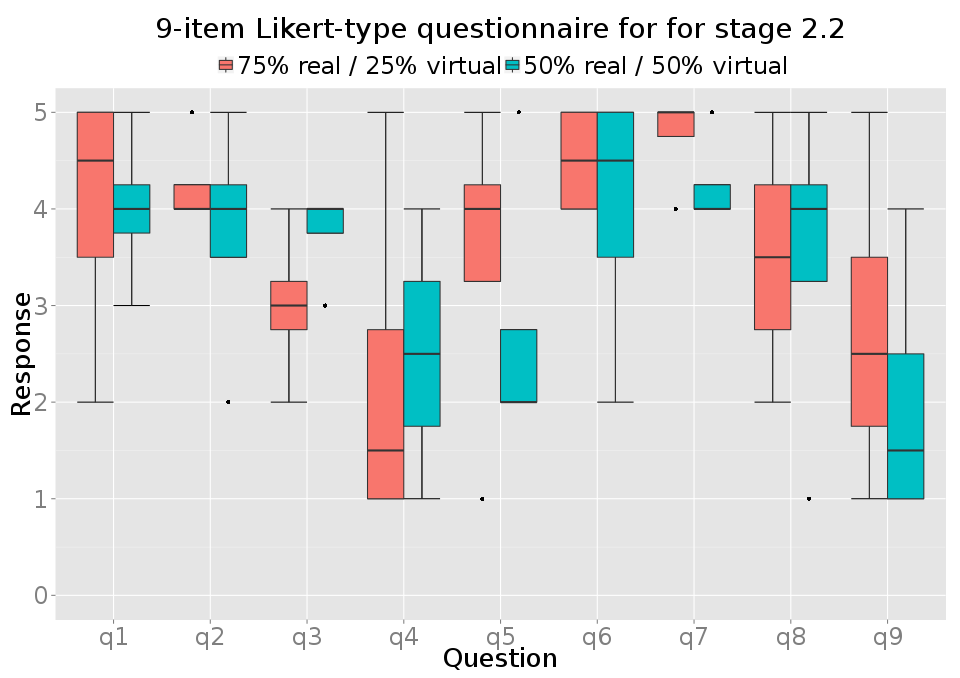
\includegraphics[width=.6\textwidth]{2.2/9-item-likert-type-questionnaire.png}
	\caption{Stage 2.2 evaluation Likert-type questionnaire results.}
	\label{9-item-likert-type-questionnaire.png}
	\end{center}
\end{figure}

These responses indicate that overall preference was mixed between the two scenarios. Although the 50/50 scenario would seem to have come out marginally ahead of the 75/25 scenario for comparison of features between past and present (q3), for reported motion sickness (q5) and for participants thinking that they didn't notice differences between real and virtual (q9), it was reported as being a less rewarding way of exploring the chapel overall (q6).

%=========================================================================================================

\subsection{Interview Transcripts}

Once again interview recordings that were transcribed after the chapel sessions gave valuable insight into the experience of the two parallel reality scenarios.

Preference between the two scenarios was evenly split, with two participants preferring the 75/25 scenario and the other two preferring the 50/50 scenario. Of those that preferred the 75/25 scenario, one explained that they felt more in control of whether they were seeing real or virtual while the other found the more obvious sudden VR movements (those where subsequent position data reported by IndoorAtlas were more than a metre or so apart) visible during the 50/50 scenario to be uncomfortable. Of those that preferred the 50/50 scenario one reported that the 75/25 scenario was \textit{``confusing to make sense of what I was seeing''} while the other found that switching to VR was less of a jump coming from 50/50, alluding to a less severe break in presence: this made him/her \textit{``more comfortable spending more time in the virtual''}. One participant mentioned that they thought they used the button more to manually transition in the 50/50 scenario because it was less jarring than in the 75/25 scenario, again supporting the notion that transitions in the 50/50 scenario resulted in a less severe break in presence.

All four of the participants agreed however that the 50/50 scenario was more engaging. Interestingly, one of the participants who reported preferring the 75/25 scenario largely because of inaccuracy of the IPS during the 50/50 scenario leading to disorientation, commented that this inaccuracy actually led to greater engagement because it would show them other parts of the VR chapel than were equivalent to their immediate surroundings, akin to Briand's `controlled schizophrenia' (see section \ref{the-mirrorshades-platform}) but completely unintentional. Two participants reported that the 50/50 scenario made differences between RW and VR more obvious, with one reporting not much discernible difference. One participant specifically mentioned how the 50/50 scenario made it more \textit{``perceptible exactly where things were''} which led to seeing themself \textit{``walking through''} (virtual) things whereas during the 75/25 scenario they would have to \textit{``switch back and forth and then realise''}.

Mimicking responses from earlier stage interviews, one participant reported experiencing motion sickness during the full immersion VR scenario when using the Xbox controller stick to turn, while for the parallel reality scenarios three of the four participants reported less motion sickness during the 50/50 scenario than the 75/25 scenario.

%=========================================================================================================

\subsection{Log Data}

\subsubsection{Considering all scenarios (seated VR and parallel reality)}

Variance in yaw once again dominated head movement for all participants during all three scenarios (seated and both parallel reality scenarios) over variance in pitch, which is illustrated in figure \ref{14-pitch-yaw-trad-75-25-50-50.png} as an example using participant 14's data showing pitch and yaw against time for the seated VR scenario at left, the 75/25 scenario in the middle and the 50/50 scenario on the right (note that the 75/25 scenario is of substantially longer duration than the other two scenarios, thus the marked difference in appearance at first glance).

\begin{figure}
	\begin{center}
	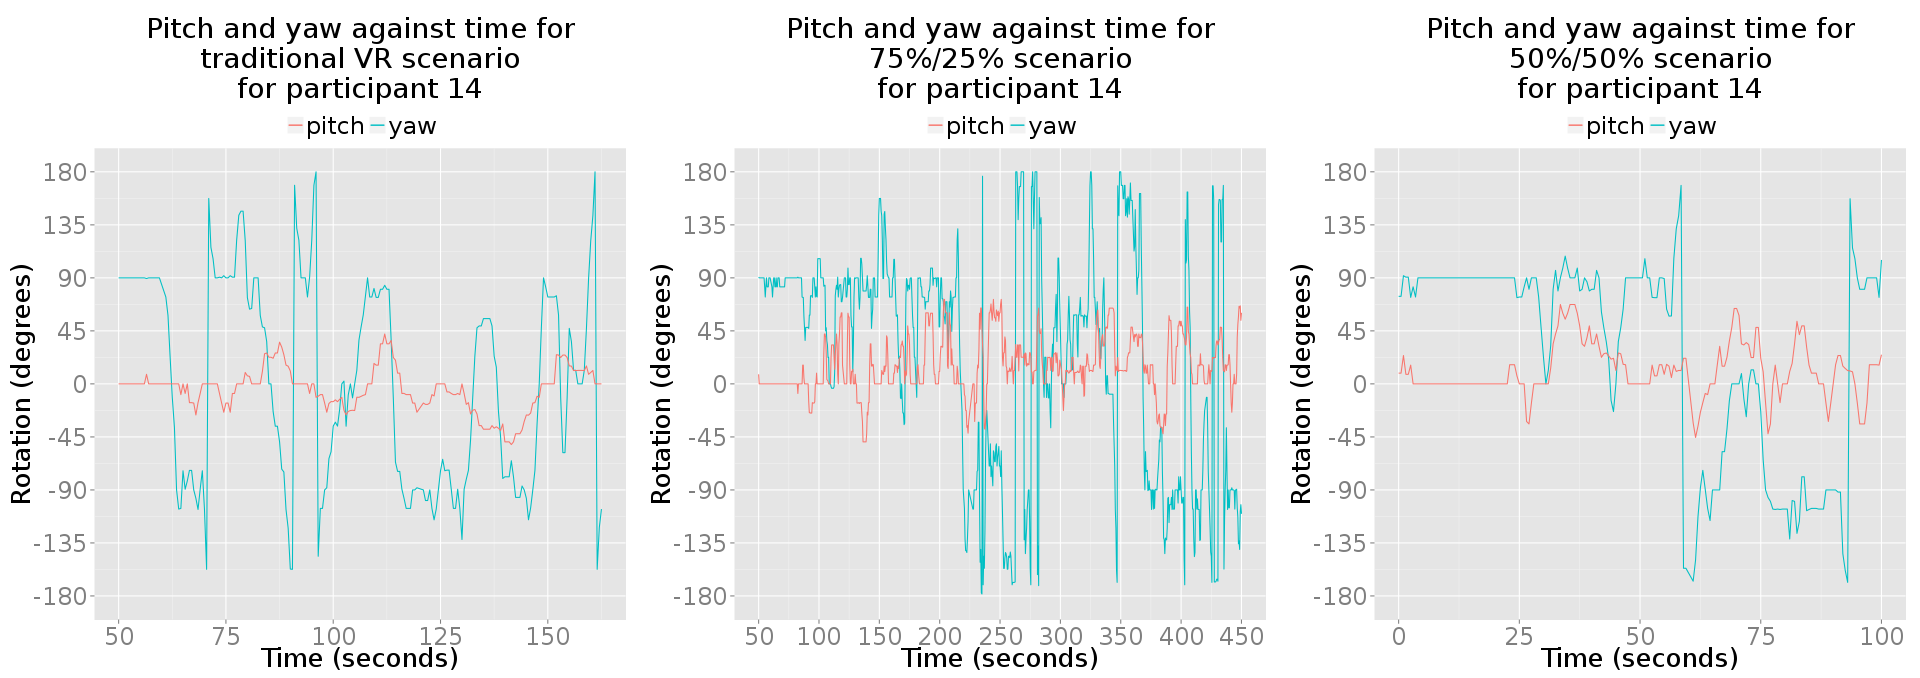
\includegraphics[width=\textwidth]{2.2/14-pitch-yaw-trad-75-25-50-50.png}
	\caption{Pitch and yaw against time for participant 14 in seated and both parallel reality scenarios.}
	\label{14-pitch-yaw-trad-75-25-50-50.png}
	\end{center}
\end{figure}

%=====================

Plots of position data upon the chapel floorplan show a similar relationship as was observed of some stage 1 participants (see section \ref{stage1-seated-vs-parallel-reality}) wherein participants approached the altar closely and even walked past it to inspect the far East walls of the chapel during the parallel reality scenarios, but did not do so during the seated VR scenario. This observation is of particular interest as walking up to the far East walls of the chapel during the parallel reality scenarios involved climbing two (real) steps (as can be seen in figure \ref{DSCN0176.jpg}), an action that intuitively one would think participants would not have enamoured the prospect of due to the nature of the video see-through solution and its associated drawbacks for ambulation. Figures \ref{16-seatedmap.png} and \ref{16-50map.png} illustrate this relationship using participant 16 as an example, for the seated VR scenario and the 50/50 scenario respectively.

\TwoFig{splodge-maps/16-seatedmap.png}{Position data (red dots) during seated VR scenario for participant 16.}{16-seatedmap.png}
       {splodge-maps/16-50map.png}{Position data (red dots) during 50/50 scenario for participant 16.}{16-50map.png}

Whilst one explanation for this behaviour, as touched upon in section \ref{stage1-seated-vs-parallel-reality}, is simply that the combination of real and virtual altar in the parallel reality scenarios drew the participants' attention more than just the virtual altar in the seated VR scenario did, enough to warrant the challenge of the steps, an additional observation herein presents a somewhat intriguing possibility. Many visitors to the chapel display a heightened reverence for the altar, not approaching it too closely nor stepping up to the platform it stands upon, presumably due to an overbearing assumption that it may be construed as disrespectful or against socially accepted etiquette to do so. However with a view that is constantly a mix of a real and a virtual environment, as in the parallel reality scenarios in this stage of the evaluation, it is conceivable that this reduced clarity or less `real' seeming nature of the altar, along with the increased interest of the combined real and virtual views, could have led participants to feel more comfortable than non parallel reality visitors to approach it more closely and even to mount its platform.

%=====================

\subsubsection{Comparing Between 75/25 and 50/50 Scenarios}

Observations that come to light when comparing log data between the two parallel reality scenarios are that all of the participants performed fewer transitions in the 50/50 scenario than in the 75/25 scenario, with the ratio between time spent in RW and VR environments showing that participants spent comparatively less time viewing VR in the 50/50 scenario than the 75/25 scenario. These values are summarised in tables \ref{times-75-25} and \ref{times-50-50} for the 75/25 and 50/50 scenarios respectively, while figures \ref{16-pitch-yaw-75-25.png} and \ref{16-pitch-yaw-50-50.png} visualise this relationship using participant 16 as an example when performing the 75/25 scenario and 50/50 scenario respectively.

\begin{figure}[h]
	\begin{center}
	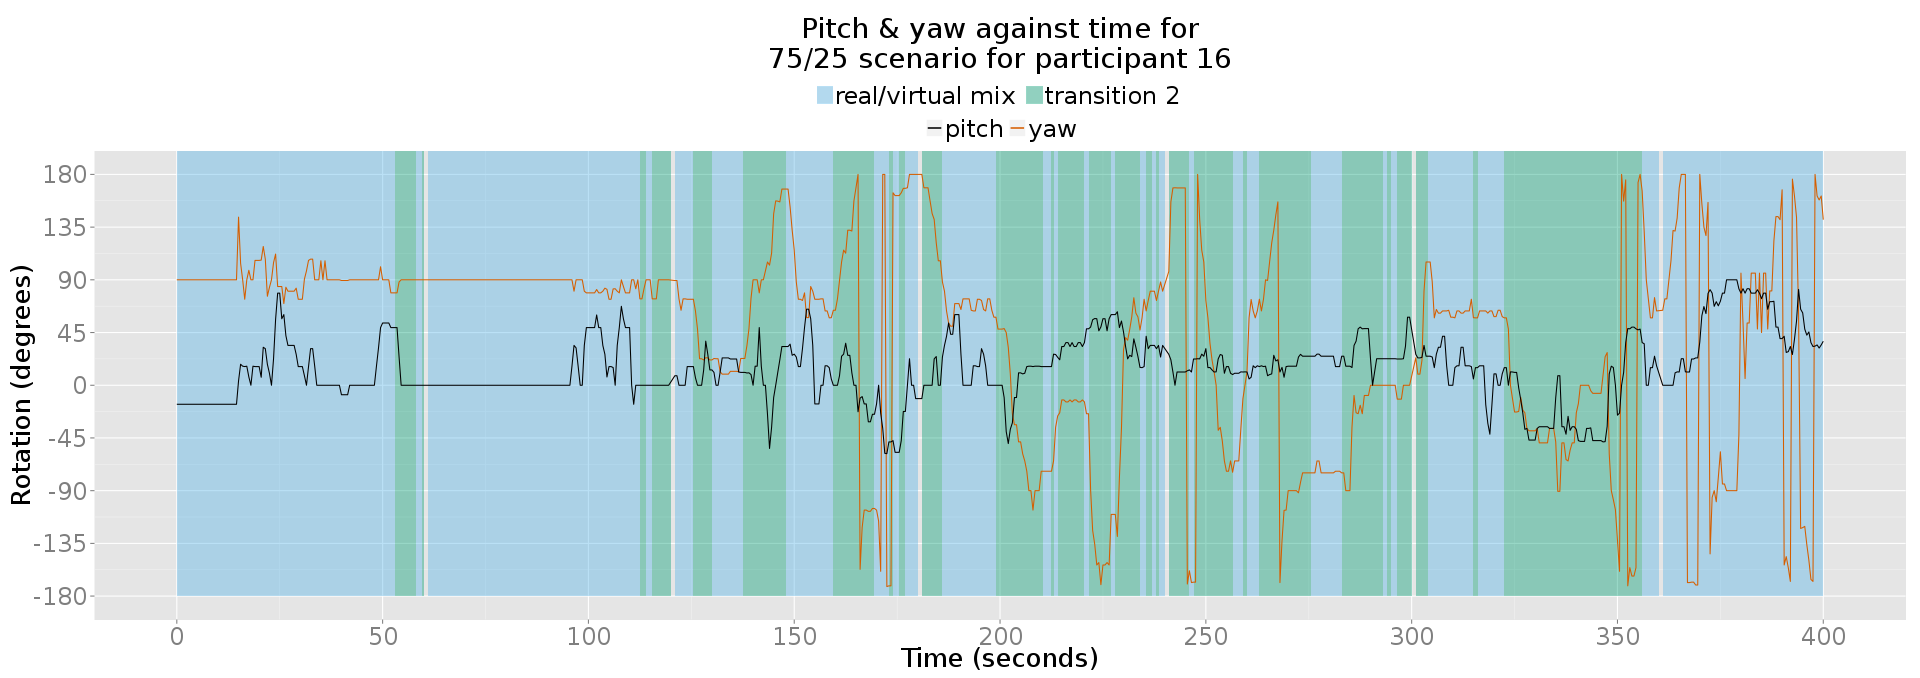
\includegraphics[width=\textwidth]{2.2/16-pitch-yaw-75-25.png}
	\caption{Pitch and yaw against time for participant 16 in 75/25 scenario, showing default/VR transitions.}
	\label{16-pitch-yaw-75-25.png}
	\end{center}
\end{figure}

\begin{figure}[h]
	\begin{center}
	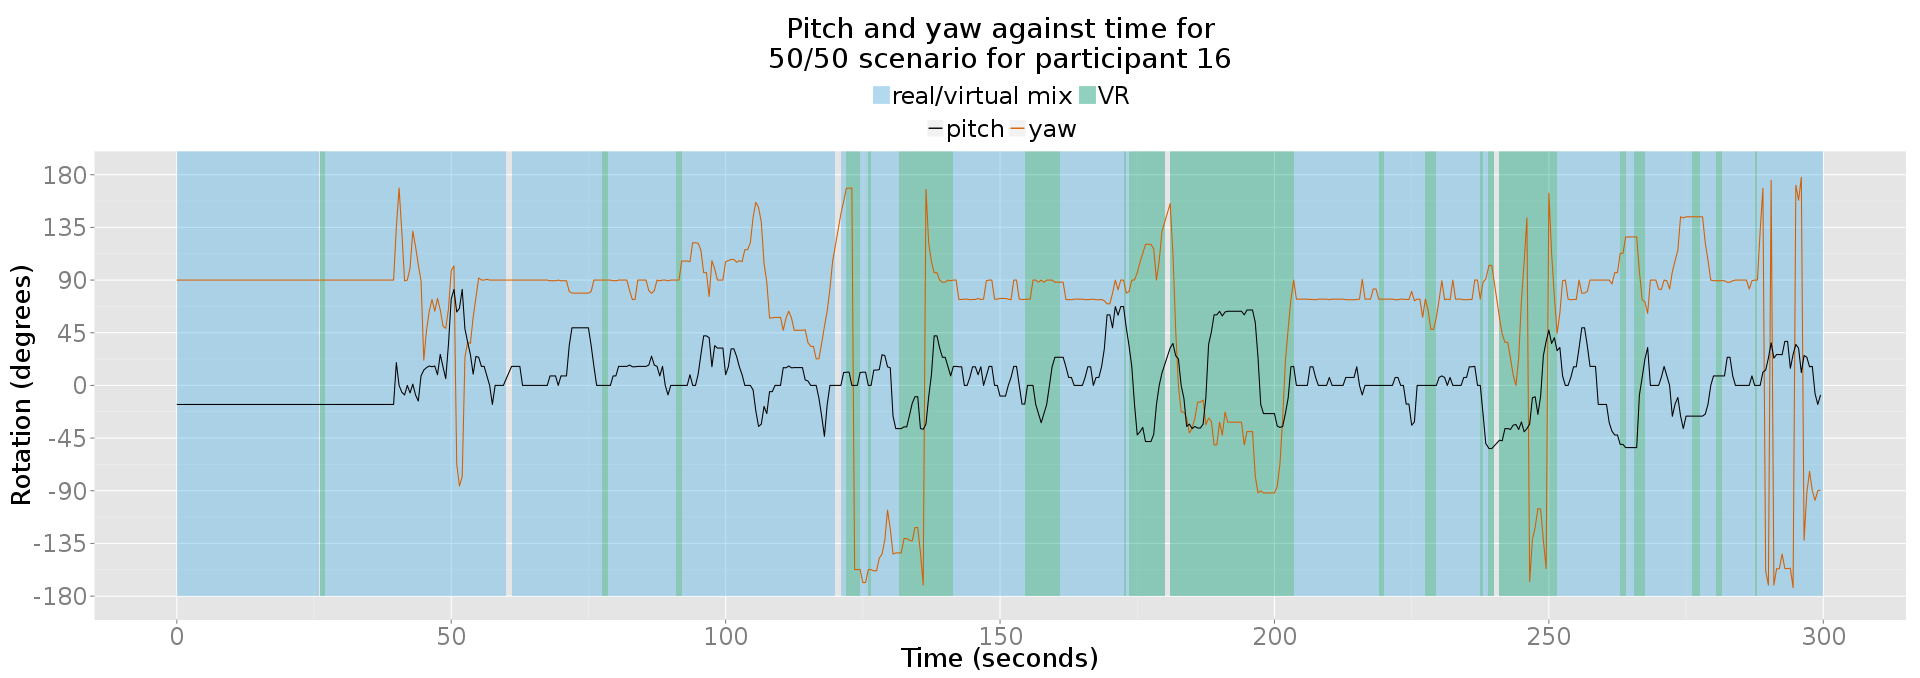
\includegraphics[width=\textwidth]{2.2/16-pitch-yaw-50-50.png}
	\caption{Pitch and yaw against time for participant 16 in 50/50 scenario, showing default/VR transitions.}
	\label{16-pitch-yaw-50-50.png}
	\end{center}
\end{figure}

In combination with interview feedback these log data are explained by the notion that the 50/50 scenario was more engaging, with participants not finding it necessary to perform transitions to VR as frequently in order to perceive enough VR stimuli to engage with it.

\newpage

When considering the distribution of variance in head pitch and yaw in relation to whether participants were viewing the default position or VR, maximum variance in stage 2.2 was no longer as closely related to the VR periods as in previous stages of the evaluation. Participant 14 in particular frequently displayed maximum variance when viewing the default position, more so even than when viewing VR, as shown by figure \ref{14-pitch-yaw-75_25.png}. While this is understandable in the sense that the participants no longer necessarily needed to perform a transition to VR in order to see a sufficient amount of the VR environment, it is worth highlighting that by allowing the user to see the VR environment in this manner means that they were simultaneously perceiving more angles of the RW environment which in earlier stages of evaluation they may not have seen as maximum variance in pitch and yaw only occurred when they were viewing VR visual stimuli.

\vspace{1.5cm}

\begin{table}[h]
\begin{center}
\begin{tabularx}{\textwidth}{c *{6}{>{\centering\arraybackslash}X}}
\toprule

\textbf{Participant} & \textbf{Number of transitions} & \multicolumn{2}{c}{\textbf{Mean duration (seconds)}} & \multicolumn{2}{c}{\textbf{Total duration (seconds)}} \\

\cmidrule(l){3-4} \cmidrule(l){5-6}

 & & \textbf{default} & \textbf{VR} & \textbf{default} & \textbf{VR} \\

\midrule

14 & 18 & 17.368 & 2.889 & 330 & 52 \\

15 & 15 & 14.656 & 3.233 & 234.5 & 48.5 \\

16 & 26 & 8.352 & 5.538 & 225.5 & 144 \\

17 & 15 & 5.013 & 1.2 & 80.2 & 18 \\

\bottomrule
\end{tabularx}
\caption{Distribution of time spent in default and VR environments for all participants during 75/25 scenario.}
\label{times-75-25}
\end{center}
\end{table}

\vspace{1.5cm}

\begin{table}[h]
\begin{center}
\begin{tabularx}{\textwidth}{c *{6}{>{\centering\arraybackslash}X}}
\toprule

\textbf{Participant} & \textbf{Number of transitions} & \multicolumn{2}{c}{\textbf{Mean duration (seconds)}} & \multicolumn{2}{c}{\textbf{Total duration (seconds)}} \\

\cmidrule(l){3-4} \cmidrule(l){5-6}

 &  & \textbf{default} & \textbf{VR} & \textbf{default} & \textbf{VR} \\

\midrule

14 & 2 & 32.5 & \textless 1 & 97.55 & \textless 1 \\

15 & 12 & 9.077 & 2.542 & 118 & 30.5 \\

16 & 18 & 11.316 & 3.661 & 215 & 65.9 \\

17 & 6 & 19.714 & 0.167 & 138 & \textless 1 \\

\bottomrule
\end{tabularx}
\caption{Distribution of time spent in default and VR environments for all participants during 50/50 scenario.}
\label{times-50-50}
\end{center}
\end{table}

\begin{figure}
	\begin{center}
	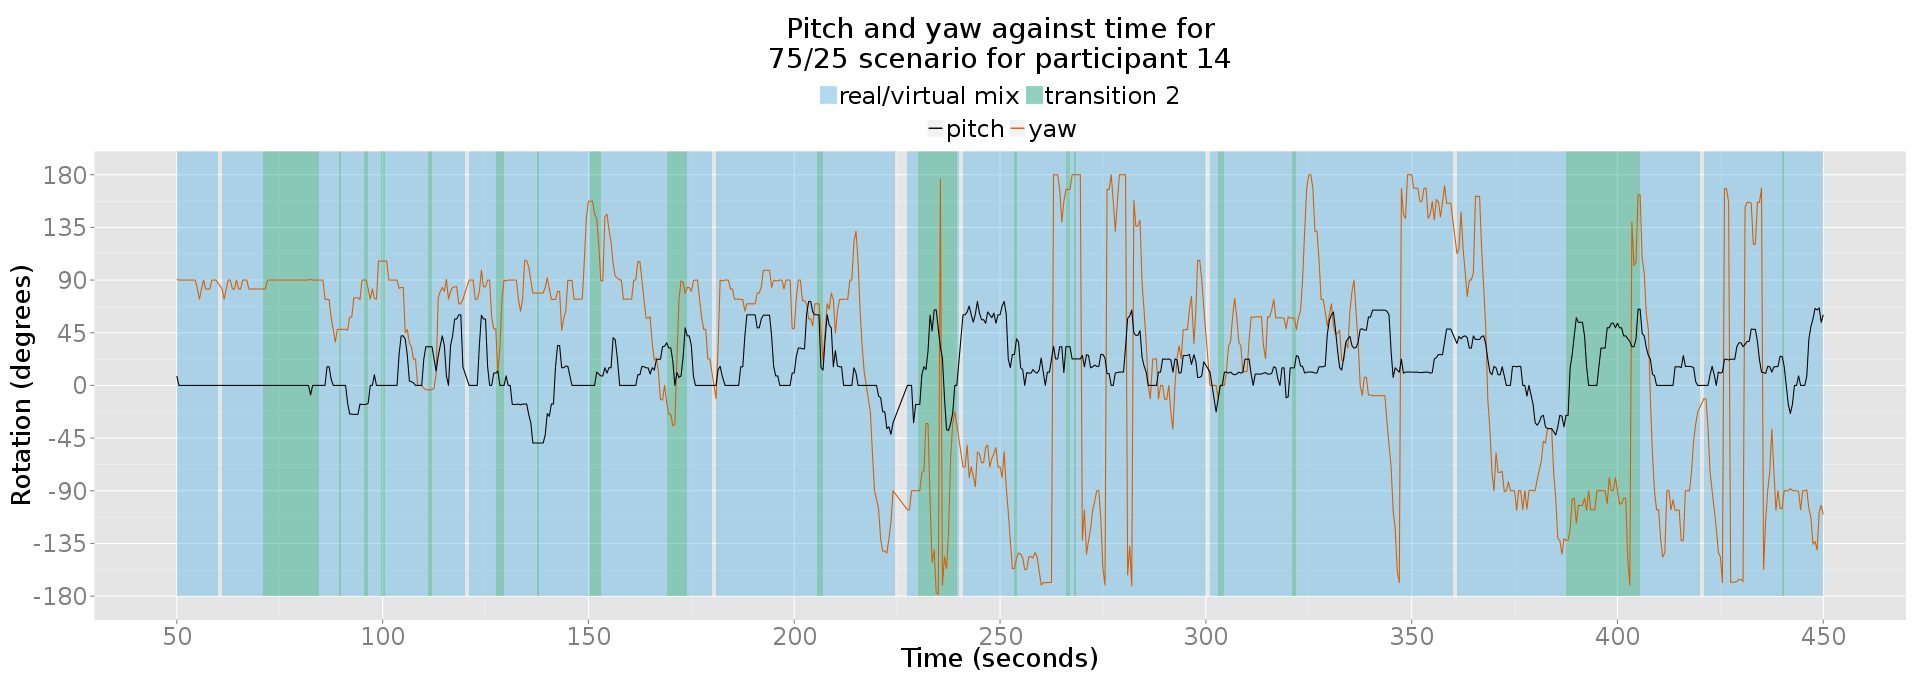
\includegraphics[width=\textwidth]{2.2/14-pitch-yaw-75_25.png}
	\caption{Pitch and yaw against time for participant 14 in 75/25 scenario, showing default/VR transitions.}
	\label{14-pitch-yaw-75_25.png}
	\end{center}
\end{figure}

%=====================

\newpage

\subsubsection{Walking and Head Movement}

Concerning the relationship between variance in head pitch and yaw compared to whether participants were actively walking, most participants exhibited similar behaviour to previous stages of evaluation with maximum variance restricted to periods in which they were standing still.

Participant 17 exhibited extremely restricted head movement (figure \ref{17-pitch-yaw-distance-moved-75-25.png}), only moving their head from looking straight ahead in the direction of movement upon reaching the altar end of the chapel and turning around to return. Intuitively one might suppose that for a participant who did not feel sure of themselves when walking with the apparatus, not having a 100\% RW view may have resulted in this static head behaviour as they would have needed to focus all of their attention on what reduced amount of the RW environment they could see in order to successfully navigate. However this participant did not report any such lack of surety in the interview, although did mention performing fewer transitions in the 50/50 scenario as they were \textit{``trying to make sure I didn't bump into anything''}. Reviewing the video recordings and ShadowPlay footage of this participant completing the 75/25 scenario showed them to walk comfortably and deliberately. The mostly static head activity is therefore as likely to be attributable to simple disinterest with the environments or misunderstanding of the purpose of the scenarios as to any restricting aspect of the apparatus or experience.

\begin{figure}[h]
	\begin{center}
	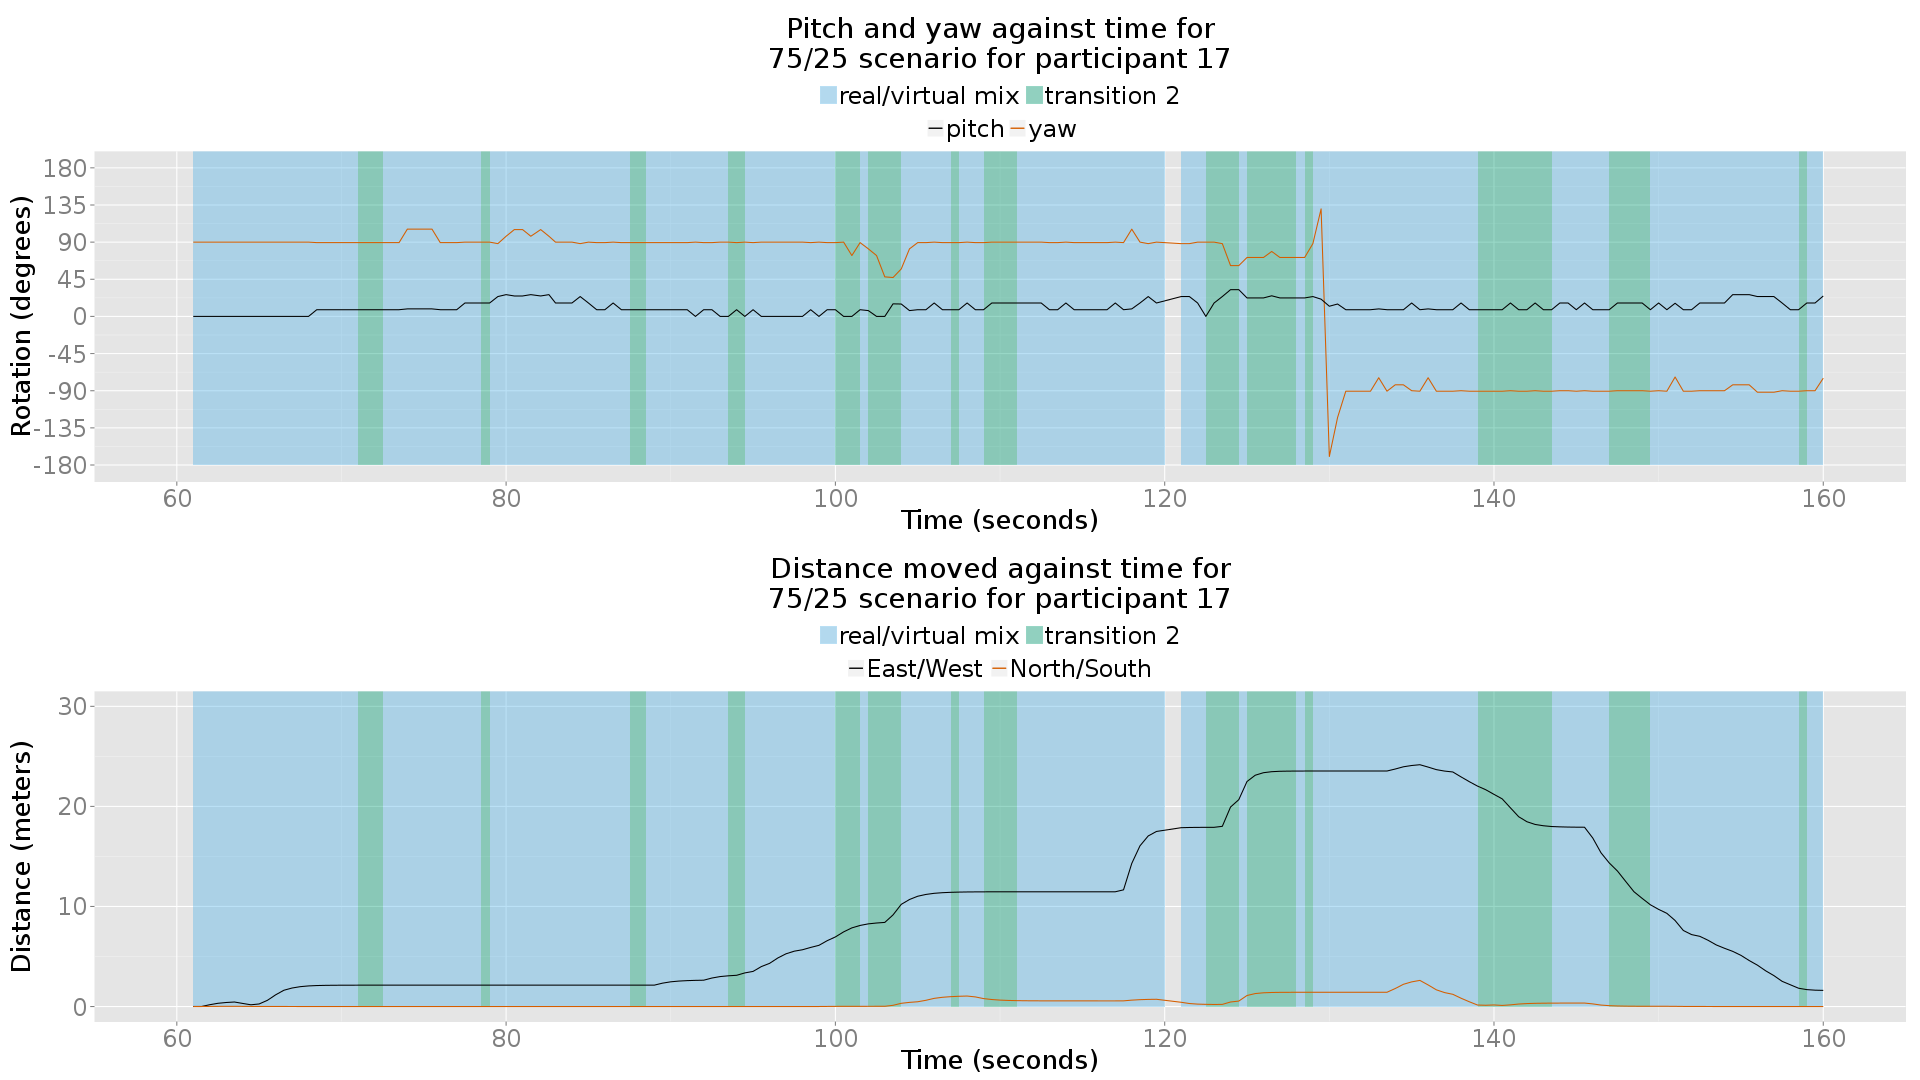
\includegraphics[width=\textwidth]{2.2/17-pitch-yaw-distance-moved-75-25.png}
	\caption{Pitch and yaw against time aligned with distance moved against time for participant 17 in 75/25 scenario, showing default/VR transitions.}
	\label{17-pitch-yaw-distance-moved-75-25.png}
	\end{center}
\end{figure}

%=========================================================================================================

\newpage

\subsection{IPQ}

When considering the IPQ results for stage 2.2 participants the seated VR scenario presents very similar results for all of SP, INV and REAL (tables \ref{sp-2-2-table}, \ref{inv-2-2-table} and \ref{real-2-2-table} respectively) to the seated VR scenario from stage 2.1 (tables \ref{sp-2-1-table}, \ref{inv-2-1-table} and \ref{real-2-1-table}). This was to be expected and confirms these values as good baseline IPQ results for a seated VR experience at the chapel.


\begin{table}
\begin{center}
\begin{minipage}[t]{.45\linewidth}
\begin{center}
\begin{tabularx}{\textwidth}{c *{3}{>{\centering\arraybackslash}X}}
\toprule

\textbf{Scenario} & \textbf{Mean} & \textbf{Standard deviation} \\

\midrule

seated & 4.3 & 0.476 \\

75/25 & 3.95 & 1.248 \\

50/50 & 4.7 & 0.739 \\

\bottomrule
\end{tabularx}
\caption{Means and standard deviations of SP for all stage 2.2 scenarios.}
\label{sp-2-2-table}
\end{center}
\end{minipage}
%
\begin{minipage}[t]{.02\linewidth}
\hfill%
\end{minipage}
%
\begin{minipage}[t]{.45\linewidth}
\begin{center}
\begin{tabularx}{\textwidth}{c *{3}{>{\centering\arraybackslash}X}}
\toprule

\textbf{Scenario} & \textbf{Mean} & \textbf{Standard deviation} \\

\midrule

seated & 4.625 & 1.299 \\

75/25 & 4.25 & 1.594 \\

50/50 & 3.25 & 1.696 \\

\bottomrule
\end{tabularx}
\caption{Means and standard deviations of INV for all stage 2.2 scenarios.}
\label{inv-2-2-table}
\end{center}
\end{minipage}

\vspace{5mm}

\begin{minipage}[t]{.45\linewidth}
\begin{center}
\begin{tabularx}{\textwidth}{c *{3}{>{\centering\arraybackslash}X}}
\toprule

\textbf{Scenario} & \textbf{Mean} & \textbf{Standard deviation} \\

\midrule

seated & 2.563 & 1.56 \\

75/25 & 1.938 & 1.593 \\

50/50 & 2.438 & 1.360 \\

\bottomrule
\end{tabularx}
\caption{Means and standard deviations of REAL for all stage 2.2 scenarios.}
\label{real-2-2-table}
\end{center}
\end{minipage}
%
\begin{minipage}[t]{.02\linewidth}
\hfill%
\end{minipage}
%
\begin{minipage}[t]{.45\linewidth}
\begin{center}
\begin{tabularx}{\textwidth}{c *{5}{>{\centering\arraybackslash}X}}
\toprule

\textbf{Scenario} & \multicolumn{2}{c}{\textbf{SP3}} & \multicolumn{2}{c}{\textbf{INV2}} \\

\cmidrule(l){2-3} \cmidrule(l){4-5}

 & \textbf{mean} & \textbf{sd} & \textbf{mean} & \textbf{sd} \\
 
\midrule

seated & 1.75 & 2.217 & 5 & 0.816 \\

75/25 & 3.75 & 1.708 & 3.5 & 1.732 \\

50/50 & 5.25 & 0.957 & 3.75 & 1.893 \\
 
\bottomrule
\end{tabularx}
\caption{Means for SP3 and INV2 for all stage 2.2 scenarios.}
\label{sp3-inv2-2-2-table}
\end{center}
\end{minipage}
\end{center}
\end{table}


SP was reduced in the 75/25 scenario to a level slightly lower than that in both parallel reality scenarios in stage 2.1, while in the 50/50 scenario there was a marked increase in SP to a level (4.7) above any other scenario in either stage, including the seated VR scenarios. This hints toward the optimistic expectation of a good parallel reality experience resulting in reduced INV but increased SP compared to a seated VR scenario, by representation of bodily actions within the RW environment leading to an increase in experienced spatial presence within the (spatially equivalent) VR environment.

INV was reduced in the 75/25 scenario and further reduced in the 50/50 scenario, as was to be expected. Interestingly however, the INV results for both parallel reality scenarios in stage 2.2 were notably higher than those for the parallel reality scenarios of stage 2.1, a discrepancy that is not contained within the higher INV for the traditional VR scenario in stage 2.2 compared to stage 2.1. When considering the difference between SP and INV for each scenario in stage 2.2, the further reduced INV value for the 50/50 scenario combined with its increased SP value indicates that in terms of the extended vacancy problem, the 50/50 scenario achieved a larger mitigation than the 75/25 scenario.

REAL was reduced in the 75/25 scenario to almost exactly the same level as both parallel reality scenarios in stage 2.1, however for the 50/50 scenario REAL was only reduced a miniscule amount (a reduction of 0.118 from 2.563 to 2.438). This implies that the increased visibility of the VR environment when perceiving the RW environment helped to enhance the perceived realness of the VR environment, possibly by mitigating the somewhat rudimentary visual quality of the virtual model by making complimentary and supporting aspects of the RW environment more prominent, masking deficiencies in the VR environment by compensating them with their RW counterparts.

When considering SP3 and INV2 in isolation, the mean SP3 for the seated VR scenario is confusingly low at 1.75 (table \ref{sp3-inv2-2-2-table}). This is especially odd considering the relatively high mean for the overall SP subscale in the seated VR scenario of 4.3 (table \ref{sp-2-2-table}). It is also completely out of line with the mean SP3 for the seated VR scenario from stage 2.1 of 4.5 (table \ref{sp-2-1-table}), which was in keeping with the overall SP mean of 4.6 (table \ref{sp3-inv2-2-1-table}) for the traditional VR scenario in stage 2.1. This oddity could be explained by possible confusion among the stage 2.2 participants the first time they completed the questionnaire over the wording of SP3, which presents a negative - \textit{``I did \textbf{not} feel present in the virtual space''} (emphasis added), anchored between \textit{``did not feel''} and \textit{``felt present''}.

%=========================================================================================================

\subsection{Graphical Performance}
\label{stage-2-2-framerates}

Once again the seated VR scenario provided the highest framerates (for the 2 participants for whom these data were captured) out of the three scenarios with an average of 53.8 fps. Both parallel reality scenarios performed slightly slower with an average of 47.7 fps during the 75/25 scenario and 48.3 fps during the 50/50 scenario. Figure \ref{framerates_2-2.png} presents these figures. The difference between the seated VR and the parallel reality scenarios was further reduced in this stage of the evaluation to an 11.3\% slowdown, lower than the 16.4\% slowdown measured in the stage 2.1 evaluation and substantially lower than the 25.2\% slowdown measured in the stage 1 evaluation.

The fact that the stage 2.2 parallel reality scenarios were predominantly rendering both real and virtual visuals simultaneously lends weight to the possibility discussed in section \ref{stage-2-1-framerates} that this style of rendering presented less computational complexity than completely culling real or virtual visuals as was the case throughout all of the stage 1 evaluations and much of the stage 2.1 evaluations. However without knowing more about the internal workings of the proprietary and `black box' Unity rendering engine, it is not possible to corroborate this idea.

\vspace{2cm}

\begin{figure}[h]
	\begin{center}
	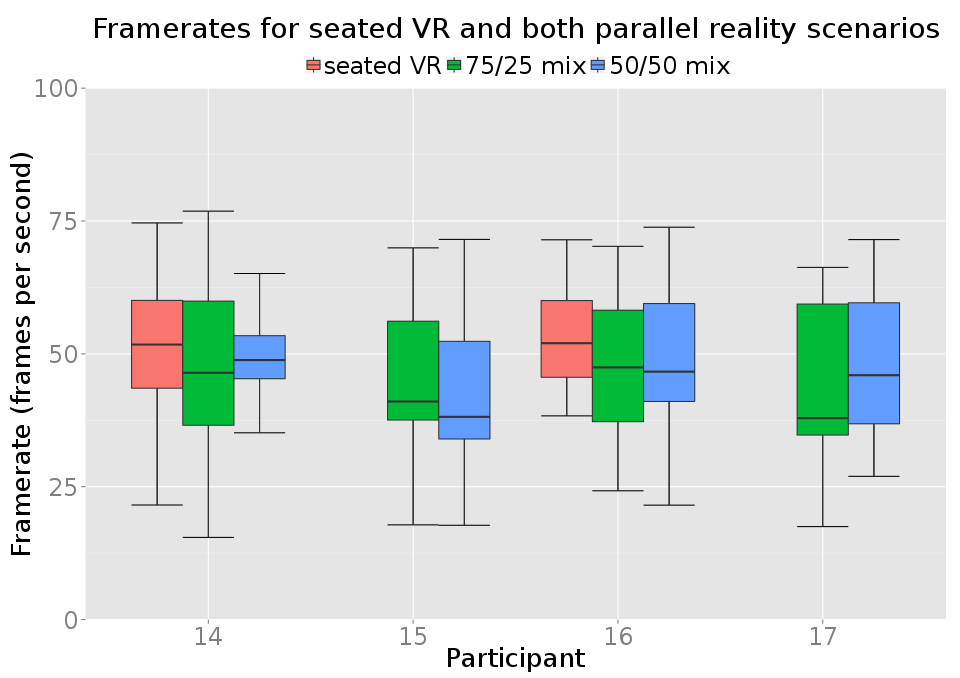
\includegraphics[width=.6\textwidth]{2.2/framerates_2-2.png}
	\caption{Framerates for seated VR and both parallel reality scenarios for all participants.}
	\label{framerates_2-2.png}
	\end{center}
\end{figure}

%=========================================================================================================

\newpage

\subsection{IndoorAtlas Performance}

Performance of IndoorAtlas was similarly high throughout both the 75/25 scenario (figure \ref{2-2-positiondeltas7525.png}) and the 50/50 scenario (figure \ref{2-2-positiondeltas5050.png}) as it was throughout the stage 2.1 evaluation. The majority of subsequent positions reported by IndoorAtlas were within 0.5 metres of the preceding position and medians approached 0 metres for all participants. However with the VR environment always being visible to some extent throughout both scenarios the occasional larger displacements would always have been perceptible (and unpleasant, according to interview feedback) to the user, whereas during the stage 2.1 evaluation the negative effect of these larger displacements was mitigated at least partly by some of them not being visible due to falling within periods when the user was perceiving 100\% RW visuals.

\TwoFig{2.2/2-2-positiondeltas7525.png}{Distance between subsequent IndoorAtlas position data for scenario with 75/25 mix.}{2-2-positiondeltas7525.png}
       {2.2/2-2-positiondeltas5050.png}{Distance between subsequent IndoorAtlas position data for scenario with 50/50 mix.}{2-2-positiondeltas5050.png}

%=========================================================================================================

\subsection{Stage 2.2 Summary}
\label{stage-2-2-summary}
This stage of the evaluation investigated the effect of changing the default view of a parallel reality experience from one that displays purely the RW environment to one that instead always includes some aspect of the VR environment, such that the user is at all times perceiving some degree of VR stimuli even when they do not consciously trigger a transition into a non-default view. This addressed the second fundamental aspect of transitions between the constituent environments of a parallel reality platform that were expected to have an effect upon the severity of breaks in presence (see section \ref{design-considerations-for-rw-vr-transitions}). Changing the default view in this manner was shown to be less disruptive, and to have a less negative affect upon the break in presence experienced when performing a transition, than the automated transition (transition 4) employed in the second of the stage 2.1 parallel reality scenarios.

Comparing the parallel reality scenarios from this stage of the evaluation to the second parallel reality scenario from the stage 2.1 evaluation in which transition 4 was used, the IPQ results indicate that the 75/25 scenario reduced SP and REAL to similar levels however the 50/50 scenario resulted in an almost imperceptible decrease in REAL and a noticeable \textit{increase} in SP. However despite the constant presence of VR visuals throughout both 75/25 and 50/50 scenarios, INV was not reduced as much as in the parallel reality scenarios from stage 2.1.

Despite these results and the fact that the 50/50 scenario was reported as allowing easier comparison between the two environments, it was considered less rewarding and was preferred less overall compared to the 75/25 scenario. In some ways this mimics the relationship between the two parallel reality scenarios in stage 2.1, where although the second led to better understanding of the two environments it did so at the cost of lessened overall comfort and enjoyment.

Fewer transitions overall during the 50/50 scenario, with participants also spending more time in total and per transition viewing the VR environment in the 75/25 scenario, support the notion that with an increased amount of VR visible in the default view participants did not feel the need to perform as frequent transitions to see the VR content. Considering the relationship observed in the stage 2.1 parallel reality scenarios of maximum variance of head movement restricted to periods in which the participants were viewing 100\% VR, reducing the participants' reliance upon performing these transitions stands to benefit participants' observation of RW components that they may otherwise have missed by perceiving only VR stimuli when looking in certain directions.

The scenario investigated in this stage of the evaluation, of presenting the two constituent environments of a parallel reality system as a mix, emerged as being useful and enjoyable by participants during the stage 2.1 evaluation in which they were able to use transition 3 to observe such situations. Although this was not the envisaged experience of parallel reality, which focussed instead upon switching wholly between discrete RW and VR environments, this stage of the evaluation has nonetheless further reinforced its utility.

However while a default view that presents \textless 100\% RW did from this evaluation seem to increase participant exposure to angles of the RW environment other than those required to walk, for a participant who feels less comfortable walking with the apparatus not having a 100\% RW view available will likely have a detrimental effect to their experience as a whole. Furthermore if a user wishes to inspect an object in the RW environment in particular detail, not being able to activate a 100\% RW view may well reduce their ability to discern detail in this object, again hampering the overall parallel reality experience.

As will be discussed further in the following chapter, these observations indicate that the ultimate realisation of a parallel reality system may in fact be one in which such a mix of RW and VR visuals are presented, in a manner more similar to familiar AR systems, but while maintaining the ability to view either complete environment individually at the total exclusion of the other.

%=========================================================================================================

\section{Best Practices for Parallel Reality}
\label{best-practices-for-parallel-reality}
The evaluations described in this and the preceding chapter have experimentally proven the feasibility and shown the value of the Mirrorshades platform, and parallel reality in general, as a new modality for the tandem exploration of real and virtual environments using a cultural heritage site as a real world use case, as well as revealing a number of indicators toward best practices for future implementations of parallel reality. With the merit of the concept compared to a seated VR experience established by the stage 1 evaluation, the stage 2.1 and 2.2 evaluations explored different implementation details of the platform to more directly inform the future development of similar systems, to allow the benefits promised by the concept to be best achieved.

Stage 2.1 assessed participant responses to several different styles of performing transitions between the constituent RW and VR environments, with a transition which furnished participants with complete control over the percentage of the visual stimuli of each environment that were presented to them emerging the clear favourite. The ability to use this transition to occupy a position between the two extremes and perceive a mix of both environments emerged as a useful and enjoyable technique, even though it was not the envisaged experience of a parallel reality platform. The introduction of brief automatic transitions from RW to VR was met negatively when assessed in terms of enjoyment and preference, but positively when assessed in terms of awareness and understanding of the relationship between the two environments.

Stage 2.2 further investigated the mix scenario, presenting VR visual stimuli to the user without their conscious invocation of a transition, with the intention of raising awareness and understanding between the environments and to cause the user to see aspects of the RW environment that they might otherwise have missed, but without introducing such the negative response as the automatic transition from stage 2.1 did. This was performed by replacing the 100\% RW default view with a view that instead presented a percentage of each environment at all times. The more extreme case of a 50\% VR/50\% RW split led to the greater increase in spatial presence within the VR environment and a barely perceptible decrease in experienced realism of the VR environment, however the 75\% RW/25\% VR split that led to less remarkable changes in IPQ results was preferred overall by the participants in interview responses.

Together, these evaluations explored the two fundamental aspects of transitions between the constituent RW and VR environments of a parallel reality system that were identified in section \ref{design-considerations-for-rw-vr-transitions} as likely to have a direct bearing on the severity of the breaks in presence, explained by the extended vacancy problem, associated with these transitions. Considering the findings of these evaluations, and drawing from observations of other aspects of the system and its use, several best practices for future parallel reality implementations are proposed:

\begin{enumerate}
	\item The combination of graphical hardware and software environment that produce the visuals displayed to the user during a parallel reality experience need to be carefully picked so as to provide sufficient quality of experience, but also need to be balanced against size, weight and heat.
	

	\item In addition to ensuring sufficient quality of virtual visuals, care should be taken to ensure that the real visuals are also presented with as much clarity as possible. In the case of a video see-through solution, there is great potential for the mediated real view to be substantially worse than that which the user perceives outwith of the parallel reality scenario, which means that the benefits of using the system need to be sufficient in order to justify notably worsening the user's experience of their real environment.
	
	\item Where inaccuracies in the positioning solution result in the requirement to perform a large movement of the virtual vantage, this movement should be effected in such a manner that the user does not perceive an unpleasant set of virtual stimuli, such as rapidly moving a large distance through the virtual environment or moving `through' virtual objects. Techniques such as reverting to purely real world visuals, blurring, dimming or similarly obfuscating virtual visuals for movements above a certain threshold distance present simple approaches to addressing this issue. Suitable notification should be presented to the user to explain the situation, as suggested for sensor quality in handheld AR platforms~\cite{Billinghurst2014}.
	
	\item In addition to intelligently handling and recovering from inaccuracies in the indoor positioning solution, every care should be taken to ensure that its normal accuracy is sufficient for the scale of comparisons expected of users and such that the lag is reduced ideally to a level beneath that which the user is capable of perceiving. Having to wait for the virtual position to `catch up' with the real position is a prominently undesirable situation.
	

	\item Both a 100\% RW and a 100\% VR view should be provided, though these do not have to be the default RW and VR positions. A 100\% VR view is diagnostic for situations in which the user wishes to perform deliberate in depth observations of a VR object, while a 100\% RW view is important both for performing similar observations of RW objects but also such that movement in the RW environment can be made as comfortable as possible for the user. Whilst improvements to HMDs and associated video see-through technologies, along with improvements to the accuracy of indoor positioning systems, will undoubtedly mitigate the detrimental effects of walking while using a video see-through HMD based parallel reality system such as Mirrorshades, the ability to revert to a 100\% RW view will ensure that the experience of walking in such a situation is presented at its most comfortable.
	\item A view that provides less than 100\% RW without the need to keep a control activated should be provided. Presenting VR visuals in this manner such that the user receives VR stimuli even without consciously thinking to perform a transition to VR or a RW/VR mix, has been shown to have a positive effect both upon participant awareness of the VR content and upon the relationship between this content and the RW environment. It also promotes observation of RW vantages that might otherwise only be seen through VR. The balance between RW and VR visuals in such a view needs to be carefully considered, as although reducing RW visuals more leads to heightened awareness and understanding of the relationship between the environments, it is the less drastically reduced RW view that was preferred overall by participants. Although this style of interaction with the constituent environments does not capture the experience originally envisaged for the parallel reality concept, its utility proven throughout the user studies indicate its worth.
	\item A method of transitioning between default RW and VR positions that allows the user to both control the speed of the transition and to stop at any intermediary level between 100\%RW/0\%VR and 0\%RW/100\%VR should be provided. This style of transition was clearly the best received throughout the evaluations and participants used this transition both to control the speed of transitions and to pause at intermediary opacities.
	





\end{enumerate}

%=========================================================================================================